\documentclass{fast-nuces-bs}

\usepackage{blindtext}
\usepackage{mathptmx}% Times Roman font
\usepackage[T1]{fontenc}
\usepackage{lipsum} 
\usepackage{sectsty}
\usepackage{tikz}
\usepackage{tikz-uml}
\usepackage{titlesec}
\usepackage{booktabs}
\usepackage{longtable}
\usepackage{array}
\usepackage{multirow}
\usepackage{xcolor}
\usepackage{float}
\usepackage{amsmath,amssymb}
\usepackage[htt]{hyphenat}
\usepackage{xurl}
\setlength{\emergencystretch}{3em}
\setlength{\tabcolsep}{3pt}
\usepackage{listings}
\usetikzlibrary{backgrounds,positioning,shapes.geometric,arrows.meta}

\lstset{
  basicstyle=\ttfamily\footnotesize,
  breaklines=true,
  frame=single,
  backgroundcolor=\color{gray!5},
  keywordstyle=\color{blue!80!black}\bfseries,
  commentstyle=\color{green!50!black}\itshape,
  stringstyle=\color{orange!80!black},
  showstringspaces=false,
  tabsize=2
}

% Custom project helper macros for consistent referencing
\newcommand{\projecttitle}{FORGE: Personalized Procedural Content Generation via Reinforcement Learning}
\newcommand{\studentone}{Rayan Ahmed (23i-0018)}
\newcommand{\studenttwo}{Rana Raza Ahmed (23i-0060)}
\newcommand{\studentthree}{Uwaid Munir (23i-2574)}

% Information about the Thesis / Report
% -----------------------------------------------------------------------------
\department{Department of Artificial Intelligence}
\faculty{FAST School of Computing}
\degreeyear{2026}
\degreemonth{October}
\degreename{Artificial Intelligence}
\campuscity{Islamabad}
\authorone{Rayan Ahmed}{23i-0018}
\authortwo{Rana Raza Ahmed}{23i-0060}
\authorthree{Uwaid Munir}{23i-2574}
\supervisor{Ms. Mehreen Javaid}
\sessionduration{2023-2027}
%\cosupervisor{}
\deanname{Dr. Dean of Computing}
\directorname{Dr. Waseem Shehzad}
\hodname{Ahmad Din}
\fypcoordinatorname{FYP Coordinator}
\title{FORGE: Personalized Procedural Content Generation via Reinforcement Learning}
%%%%%%%%%%%%%%%%%%%%%%%%%%%%%%%%%%%%%%%%%%%%%%%%%%%%%%%%%%%%%%%%%%%%%%%%%%%%%%%

\begin{document}

\clearpage
\pagenumbering{roman}
\chapter*{Students' Submission}
\addcontentsline{toc}{chapter}{Students' Submission}

We certify that this report is submitted as the FYP-1 mid-evaluation report for the project titled \textit{\projecttitle}.

\vspace{1.5cm}

\begin{tabular}{p{0.5\textwidth}p{0.45\textwidth}}
\textbf{Student 1:} \studentone & \textbf{Signature:} \rule{0.28\textwidth}{0.4pt}\\[1.5cm]
\textbf{Student 2:} \studenttwo & \textbf{Signature:} \rule{0.28\textwidth}{0.4pt}\\[1.5cm]
\textbf{Student 3:} \studentthree & \textbf{Signature:} \rule{0.28\textwidth}{0.4pt}\\[1.5cm]
\end{tabular}

\vspace{1.5cm}
\noindent\textbf{Date of Submission:} October 15, 2026

\chapter*{Anti-Plagiarism Statement}
\addcontentsline{toc}{chapter}{Anti-Plagiarism Statement}

The project team certifies that this report is our original work and that all external sources, algorithms, libraries, frameworks, academic publications, and tool-assisted contributions utilized in preparing this report and developing the software have been formally and appropriately acknowledged and cited. 

We confirm that this document adheres strictly to the academic integrity and anti-plagiarism regulations established by the National University of Computer and Emerging Sciences (FAST-NUCES) and the Higher Education Commission (HEC) of Pakistan.

\vspace{2cm}

\begin{tabular}{p{0.5\textwidth}p{0.45\textwidth}}
\studentone & \textbf{Signature:} \rule{0.28\textwidth}{0.4pt}\\[1.5cm]
\studenttwo & \textbf{Signature:} \rule{0.28\textwidth}{0.4pt}\\[1.5cm]
\studentthree & \textbf{Signature:} \rule{0.28\textwidth}{0.4pt}
\end{tabular}

\chapter*{Authors' Declaration}
\addcontentsline{toc}{chapter}{Authors' Declaration}

We hereby declare that the software development, algorithmic designs, mathematical formulations, experimental pipelines, and engineering documentation presented in this FYP-1 Mid-Term Report titled \textit{\projecttitle} represent the authentic and collaborative work carried out by the undersigned project team at the Department of Artificial Intelligence, FAST School of Computing, National University of Computer and Emerging Sciences, Islamabad.

We declare that this submission reflects the actual state of development achieved during Iterations 1 and 2 (Weeks 1 through 10). All external third-party packages (including Godot Engine 4.3, Stable-Baselines3, PyTorch, and Gymnasium), open-source assets, and assistive AI tools used under Level 2 AI-Assisted Development are explicitly disclosed in Chapter~\ref{chap:mgmt} and the corresponding Appendices.

\vspace{2cm}

\begin{tabular}{p{0.5\textwidth}p{0.45\textwidth}}
\studentone & \textbf{Signature:} \rule{0.28\textwidth}{0.4pt}\\[1.5cm]
\studenttwo & \textbf{Signature:} \rule{0.28\textwidth}{0.4pt}\\[1.5cm]
\studentthree & \textbf{Signature:} \rule{0.28\textwidth}{0.4pt}
\end{tabular}

\chapter*{Abstract}
\addcontentsline{toc}{chapter}{Abstract}

Procedural Content Generation (PCG) in video games has largely transitioned from brittle rule-based grammars to learned policies via Reinforcement Learning (PCGRL). However, prevailing PCGRL frameworks synthesize environments conditioned on static designer-authored target vectors or optimize for an aggregate average player, ignoring individual differences in motor skill, risk tolerance, and combat pacing. Concurrently, conventional Dynamic Difficulty Adjustment (DDA) mechanisms rely on simplistic, reactive scalar multipliers that frequently trigger perceptible rubber-banding and break player immersion.

This project presents \textbf{FORGE} (\textit{Personalized Procedural Content Generation via Reinforcement Learning}), an end-to-end, closed-loop adaptive dungeon synthesizer developed in the Godot 4.x engine for 2D top-down combat roguelikes. FORGE continuously profiles in-session gameplay telemetry (clearing time, death count, and damage taken) which, with the current difficulty settings and run depth, forms the 8-dimensional input of a Proximal Policy Optimization (PPO) policy. The policy outputs a structured 7-dimensional combat difficulty action vector controlling continuous enemy attributes (health, damage, speed, aggro radius), environmental hazard density, resource scarcity, and room count. To eliminate sim-to-real latency and external runtime dependencies, FORGE couples an offline Python training pipeline (Gymnasium, Stable-Baselines3) with an embedded, zero-latency pure-GDScript neural network forward pass executing in about $0.2$\,ms. 

To overcome initial cold-start volatility, FORGE introduces a 5-floor weighted calibration protocol that establishes an empirical baseline combat rating ($CR_0$) before closed-loop adaptation activates. For the FYP-1 Mid-Term Evaluation, the project team implemented and verified: (1) cohesive pixel-art dungeon aesthetics, trauma-decay camera shake, and color-coded floating combat text; (2) multi-archetype combat dynamics featuring Melee Crawlers and Ranged Pyromancers with telegraphed fireball projectiles alongside a player invulnerability dodge roll; (3) a live telemetry defense overlay with a deterministic static roguelike baseline toggle; and (4) an automated headless Godot continuous integration (CI) pipeline validating 100\% topological solvability across randomized seeds. Testing confirms zero-crash fallback and 60\,FPS execution, demonstrating the feasibility of personalized closed-loop procedural game generation.

\chapter*{Acknowledgments}
\addcontentsline{toc}{chapter}{Acknowledgments}

The authors express their deepest gratitude to our faculty supervisor, \textbf{Ms. Mehreen Javaid}, for her invaluable technical mentorship, constructive critiques, and continuous guidance throughout the conceptualization, system architecture design, and mid-stage execution of Project FORGE. Her insistence on rigorous literature grounding and empirical validation significantly strengthened the academic and engineering foundations of this work.

We extend our sincere thanks to the FYP Evaluation Committee and the faculty members of the Department of Artificial Intelligence and FAST School of Computing, National University of Computer and Emerging Sciences, Islamabad. Their constructive feedback during the Proposal Defense provided the direct impetus for our expanded Dynamic Difficulty Adjustment (DDA) literature review, the introduction of multi-archetype enemy behaviors, and our automated continuous integration testing pipeline.

Finally, we express our profound appreciation to our families, colleagues, and peer playtesters whose enduring encouragement, patience, and preliminary gameplay feedback have been vital to the ongoing success of this Final Year Project.

\chapter*{Executive Summary}
\addcontentsline{toc}{chapter}{Executive Summary}

\section*{Strategic Context and Motivation}
Procedural Content Generation via Reinforcement Learning (PCGRL) has emerged as a state-of-the-art methodology for synthesizing complex, replayable video game levels. Despite substantial advances in benchmark environments such as \texttt{gym-pcgrl}, mainstream procedural level generators remain inherently static: they optimize level layouts against an abstract, aggregate statistical average. In reality, player populations exhibit high variance in mechanical dexterity, tactical risk tolerance, spatial navigation speed, and frustration thresholds. Static generation inevitably under-challenges seasoned veterans (inducing boredom) and overwhelms novices (inducing anxiety), violating Csikszentmihalyi's psychological conditions for player flow. Concurrently, existing Dynamic Difficulty Adjustment (DDA) systems deployed in commercial titles rely on reactionary, transparent heuristic triggers (such as scalar health/damage multipliers) that produce jarring rubber-banding effects and undermine player agency.

\section*{Project Vision and Solution Architecture}
Project \textbf{FORGE} (\textit{Personalized Procedural Content Generation via Reinforcement Learning}, Project ID: F26-012-FORGE) bridges this gap by engineering an online, closed-loop procedural dungeon generator for 2D top-down action roguelikes built in Godot 4.x. FORGE establishes a two-stage decoupled architecture:
\begin{enumerate}
    \item \textbf{Stage 1: Deterministic Spatial Topology Synthesis.} A random-walk-with-branching room layout algorithm attaches every new room to an already placed room through a matching door pair, so each floor is a connected room graph by construction; a headless CI harness verifies start-to-exit reachability with a breadth-first search over the door graph on 500 seeds.
    \item \textbf{Stage 2: Closed-Loop Reinforcement Learning Combat Adapter.} A Proximal Policy Optimization (PPO) policy observes an 8-dimensional state (three in-session player signals: clearing time, death count and damage-taken ratio; the four current difficulty settings: enemy health, enemy damage, hazard density and room count; and run depth) and synthesizes a structured 7-dimensional difficulty action vector controlling continuous enemy combat attributes (health, damage, speed, aggro radius), environmental hazards, and room count.
\end{enumerate}
To avoid sim-to-real latency and eliminate external Python or ONNX runtime dependencies on client machines, FORGE employs an offline training pipeline in Gymnasium with Stable-Baselines3, exporting actor weights to a compact JSON file. At runtime, an embedded, zero-overhead pure-GDScript neural network forward pass computes difficulty adjustments in about $0.2$\,ms.

\section*{Committee Feedback Resolution and Mid-1 Deliverables}
Following the Proposal Defense in which Project FORGE was approved with minor modifications, the team conducted an exhaustive systematic review of 32 sources (peer-reviewed publications, preprints and foundational texts) across PCGRL and DDA literature. During Iterations 1 and 2 (Weeks 1 through 10), the team fulfilled all mid-term commitments mandated by the FYP Committee and the FAST School of Computing CI/CD Directive:
\begin{itemize}
    \item \textbf{Visual Aesthetic Overhaul and Combat Juice:} Replaced preliminary geometric placeholder shapes with custom pixel-art top-down sprites (\texttt{player.png}, \texttt{enemy\_crawler.png}, \texttt{enemy\_pyromancer.png}, dungeon stone flagstones), integrated trauma-decay camera shake ($T \in [0, 1]$), color-coded floating combat text (damage, taken, healing), and professional typography (Cinzel and Inter fonts).
    \item \textbf{Multi-Archetype Combat Dynamics:} Introduced distinct tactical adversary behaviors---a direct-pursuit Melee Crawler and a kiting Ranged Pyromancer casting telegraphed fireball projectiles---counterbalanced by a player invulnerability dodge roll ($0.2$\,s dash, $1.0$\,s cooldown).
    \item \textbf{5-Floor Cold-Start Calibration Protocol:} Implemented a weighted initial profiling phase (Floors 1--5) calculating a composite Combat Rating ($CR_0 \in [10, 95]$) with escalating difficulty weights ($\vec{w} = [1.0, 1.5, 2.0, 2.5, 3.0]$) to prevent early difficulty thrashing before closed-loop PPO takes over at Floor 6.
    \item \textbf{Static Non-Adaptive Roguelike Baseline Mode:} Developed an in-engine toggle in the live Defense Telemetry Overlay enabling evaluators and players to benchmark the adaptive PPO generator against a deterministic $+8\%$ per-floor stat progression baseline.
    \item \textbf{Automated Headless Godot CI Pipeline:} Engineered a GitHub Actions continuous integration workflow verifying headless script compilation and validating 100\% topological solvability across 500 randomized seeds on every commit.
\end{itemize}

\section*{Early Validation, Risk Governance, and FYP-2 Horizon}
Comprehensive testing demonstrated that the pure-GDScript forward pass executes in about $0.2$\,ms (mean $0.21$\,ms, maximum $0.36$\,ms) with 0\% frame drops below 60\,FPS. In fault-injection stress tests (missing or corrupted weights JSON), the engine smoothly engaged a rule-based heuristic fallback without crashing. Telemetry governance operates entirely client-side using local JSON serialization, collecting zero Personally Identifiable Information (PII).

With Mid-1 milestones fully baselined and validated, the remaining project roadmap focuses on:
\begin{itemize}
    \item \textbf{FYP-1 Final (Iteration 3, Weeks 11--14):} Expanding the combat ecosystem to 5 archetypes (adding Brute, Skirmisher, and Swarmer), migrating the telemetry store to SQLite, and training the empirical Judge regressor ($\text{MAE} \le 0.15$) with live polynomial TreeSHAP feature attribution inside Godot.
    \item \textbf{FYP-2 Mid (Iteration 4, Weeks 15--26):} Implementing the in-run equipment shop economy, re-validating the Judge model against it, system integration testing, and non-functional performance benchmarking.
    \item \textbf{FYP-2 Final (Iteration 5, Weeks 27--32):} Conducting a formal 10-participant human User Acceptance Testing (UAT) study using the Game Engagement Questionnaire (GEQ) and Player Experience of Need Satisfaction (PENS) instruments.
\end{itemize}
Project FORGE is on schedule, on budget, and fully aligned with all academic and engineering rubrics of FAST-NUCES.


\tableofcontents
\listoffigures
\listoftables
\chapter*{List of Abbreviations}
\addcontentsline{toc}{chapter}{List of Abbreviations}

\begin{longtable}{ll}
\toprule
\textbf{Abbreviation} & \textbf{Full Description} \\
\midrule
AI & Artificial Intelligence \\
A2C & Advantage Actor-Critic \\
BSP & Binary Space Partitioning \\
CCP & Complex Computing Problem \\
CI/CD & Continuous Integration / Continuous Deployment \\
CLO & Course Learning Outcome \\
CR & Combat Rating (e.g., $CR_0$ Initial Combat Rating) \\
DDA & Dynamic Difficulty Adjustment \\
DER & Difficulty Error Rate \\
DQN & Deep Q-Network \\
ERD & Entity-Relationship Diagram \\
FAST & Foundation for Advancement of Science and Technology \\
FPS & Frames Per Second \\
FR & Functional Requirement \\
FYP & Final Year Project \\
GDScript & Godot Engine Scripting Language \\
GEQ & Game Engagement Questionnaire \\
GUI & Graphical User Interface \\
HEC & Higher Education Commission (Pakistan) \\
HUD & Heads-Up Display \\
JSON & JavaScript Object Notation \\
MAE & Mean Absolute Error \\
MDP & Markov Decision Process \\
ML & Machine Learning \\
MLP & Multilayer Perceptron \\
NFR & Non-Functional Requirement \\
NTRL & RL-based encounter-generation method of Romeo and Bagdanov \\
NUCES & National University of Computer and Emerging Sciences \\
PCG & Procedural Content Generation \\
PCGRL & Procedural Content Generation via Reinforcement Learning \\
PENS & Player Experience of Need Satisfaction \\
PII & Personally Identifiable Information \\
PPO & Proximal Policy Optimization \\
R\&D & Research and Development \\
RL & Reinforcement Learning \\
SAC & Soft Actor-Critic \\
SDS & Software Design Specification \\
SHAP & Shapley Additive Explanations (TreeSHAP) \\
SRS & Software Requirements Specification \\
TTK & Time To Kill \\
UAT & User Acceptance Testing \\
UML & Unified Modeling Language \\
WBS & Work Breakdown Structure \\
\bottomrule
\end{longtable}


\cleardoublepage
\pagenumbering{arabic}
\chapter{Introduction and Project Vision}
\label{chap:intro}

\section{Project Overview}
Video games represent one of the most prominent sectors of modern entertainment, increasingly relying on Procedural Content Generation (PCG) to maintain long-term replayability, mitigate content exhaustion, and reduce escalating production overhead. While early algorithmic generation depended on deterministic cellular automata, grammars, or Binary Space Partitioning (BSP), recent developments have advanced toward learned policies trained through Reinforcement Learning (PCGRL)~\cite{khalifa2020pcgrl}. 

However, existing PCGRL systems typically generate game content optimized for an abstract, aggregate statistical average or require human designers to author explicit target vectors manually~\cite{earle2021controllable}. When real human players interact with such systems, the static nature of generation inevitably conflicts with the broad distribution of human motor skill, tactical risk tolerance, spatial navigation pacing, and combat capabilities.

Project \textbf{FORGE} (\textit{Personalized Procedural Content Generation via Reinforcement Learning}, Project ID: F26-012-FORGE) is an online, closed-loop adaptive dungeon synthesizer engineered for 2D top-down combat roguelikes within the Godot 4.x engine. Rather than generating content offline or relying on intrusive questionnaires, FORGE actively and passively records in-session gameplay telemetry (clearing time, death count, and damage-taken ratio). Together with the current difficulty settings and run depth, this telemetry forms an 8-dimensional observation that conditions a Proximal Policy Optimization (PPO)~\cite{schulman2017proximal} actor policy that dynamically outputs a continuous 7-dimensional difficulty action vector. This action vector modulates adversary combat attributes (health, damage, speed, aggro radius), environmental hazards, and dungeon complexity in real time. 

By marrying an offline Python training pipeline with a zero-latency pure-GDScript neural network forward pass, FORGE creates an authentic, responsive game environment that sustains player engagement without causing perceptible difficulty thrashing.

\section{Problem Statement}
Procedural level generation in combat dungeon crawlers faces a critical trade-off between infinite variety and calibrated challenge:
\begin{enumerate}
    \item \textbf{The One-Size-Fits-All Failure Mode:} Content tuned for a nominal player inevitably under-challenges highly skilled veterans (inducing boredom and disengagement) and over-penalizes novice players (inducing anxiety, frustration, and premature churn).
    \item \textbf{The Brittle Rubber-Banding Fallacy:} Traditional Dynamic Difficulty Adjustment (DDA) systems adjust game parameters reactively using hardcoded threshold triggers (such as scalar health or damage multipliers). These systems are readily transparent to players, produce jarring swings in difficulty, and undermine player agency by penalizing proficient play.
    \item \textbf{The PCGRL Personalization Void:} While reinforcement learning has proven effective for synthesizing topologically valid level structures, prevailing PCGRL algorithms operate open-loop: they do not ingest continuous in-session human telemetry to adapt the generated challenges dynamically to individual capabilities.
\end{enumerate}

\subsection*{Central Research Question}
To address these interrelated deficiencies, Project FORGE is guided by the following central research question:
\begin{quote}
\textit{``Can a reinforcement-learning-based procedural content generation system utilize continuous in-session gameplay telemetry to infer an individual player's behavioral profile and synthesize solvable dungeon content whose multi-dimensional combat and environmental difficulty is measurably better matched to that player's observed capability than non-personalized procedural baselines?''}
\end{quote}

\section{Problem Context and Motivation}
The psychological foundation of interactive entertainment rests upon the Theory of Flow in digital games~\cite{michailidis2018flow}. Flow represents an optimal mental state characterized by deep absorption and intrinsic motivation, achieved when the challenges presented by an activity precisely balance the actor's perceived skills. When challenges outstrip capability, anxiety ensues; conversely, when skill dominates challenge, boredom terminates engagement.

In action roguelikes (e.g., \textit{Hades}, \textit{The Binding of Isaac}, \textit{Enter the Gungeon}), per-run replayability is paramount. However, players possess vastly different learning curves. A rigid difficulty curve leads to asymmetric retention: novices abandon the game within the first few floors, while experts speedrun through content without experiencing tactical resistance. 

Attempts by commercial studios to mitigate this via reactive DDA (such as Capcom's Dynamic Rank in \textit{Resident Evil 4} or Valve's AI Director in \textit{Left 4 Dead}~\cite{zohaib2018dynamic, mortazavi2024dda}) highlight the industry's demand for adaptive pacing. However, heuristic rule sets often create artificial difficulty adjustments that break immersion. There is an acute engineering and research demand for an AI system that treats difficulty as an organic, multi-attribute parameter space—incorporating adversary speed, aggro geometry, hazard density, and tactical archetype composition—learned and navigated via deep reinforcement learning.

\section{Project Vision}
The overarching vision of Project FORGE is to establish a unified, open-source, reproducible paradigm for player-conditioned procedural generation in action games. FORGE envisions a gameplay experience where:
\begin{itemize}
    \item Game content seamlessly conforms to the player's evolving flow channel without requiring manual difficulty selection menus (e.g., Easy, Normal, Hard).
    \item The adaptation mechanism operates unobtrusively, preserving the principle of ``change blindness'' so that players perceive the world as challenging yet fair, attributing their survival to personal mastery rather than patronizing AI assistance.
    \item The generative system runs deterministically on client hardware with zero cloud latency, zero external server dependencies, and rigorous mathematical guarantees of topological reachability and solvability.
\end{itemize}

\section{Project Objectives}
To realize this vision, the project team formulated six specific, measurable engineering and research objectives:
\begin{itemize}
    \item \textbf{OBJ-1 (Continuous Telemetry \& Profiling Engine):} Construct an unobtrusive telemetry logging framework capturing fine-grained in-session performance metrics (room traversal velocity, hit-to-damage ratio, trap trigger frequency, death count) at 60\,FPS without frame drops.
    \item \textbf{OBJ-2 (Reinforcement Learning Difficulty Policy):} Train a stable PPO policy in a simulated multi-room Gymnasium environment capable of mapping 8-dimensional observation states (three player-performance signals, four current difficulty settings and run depth) into smooth 7-dimensional difficulty parameter updates.
    \item \textbf{OBJ-3 (Two-Stage Decoupled Dungeon Synthesizer):} Implement a modular generator separating spatial topology generation from combat encounter placement, ensuring topological reachability (connected by construction and verified by a breadth-first search over the door graph on 500 CI seeds).
    \item \textbf{OBJ-4 (Multi-Archetype Combat Dynamics):} Develop distinct adversary behavioral archetypes (Melee Crawlers, Ranged Pyromancers) with telegraphed combat tells, projectile collisions, and active player defensive mechanics (dodge roll).
    \item \textbf{OBJ-5 (Automated Continuous Integration Solvability Testing):} Establish a headless CI/CD pipeline using GitHub Actions that compiles Godot scripts, executes headless room solvability simulations across 500 random seeds, and verifies policy export integrity on every commit.
    \item \textbf{OBJ-6 (Empirical \& Psychometric Validation):} Establish a formal verification framework evaluating both objective performance metrics (solvability rate, difficulty error rate $\text{DER}$, inference latency) and standardized psychometric instruments (Game Engagement Questionnaire, Player Experience of Need Satisfaction).
\end{itemize}

\section{Project Scope}\label{sec:scope}
To ensure rigorous progress while avoiding scope creep, the project scope is formally partitioned across project milestones as shown in Table~\ref{tab:scope_matrix}.

\begin{table}[!htbp]
\centering
\caption{FORGE Project Scope Boundary and Delivery Matrix}
\label{tab:scope_matrix}
\small
\begin{tabular}{p{0.32\textwidth}p{0.32\textwidth}p{0.28\textwidth}}
\toprule
\textbf{In-Scope: Mid-1 (Completed)} & \textbf{In-Scope: Final-1 / FYP-2} & \textbf{Explicitly Out-of-Scope} \\
\midrule
1. Pixel-art dungeon sprites \& aesthetic juice (camera shake, damage numbers). & 1. Expanded 5-archetype enemy ecosystem (Brute, Skirmisher, Swarmer). & 1. 3D graphics rendering or VR/AR interfaces. \\
2. Multi-archetype combat: Melee Crawler \& Ranged Pyromancer with projectiles. & 2. In-run equipment shop economy with currency (\textit{Forge Embers}) (Mid-2). & 2. Online/LAN multiplayer networking. \\
3. Player dodge roll with invulnerability frames and cooldown. & 3. Rule-based BSP generator comparison baseline. & 3. Procedural music or audio synthesis. \\
4. 5-Floor Cold-Start Calibration Protocol with weighted $CR_0$ baseline. & 4. Migration of telemetry store from flat JSON to embedded SQLite. & 4. Client-side continuous policy training (RL training remains offline). \\
5. In-engine pure-GDScript PPO actor forward pass (about $0.2$\,ms). & 5. Supervised empirical Judge model ($\text{MAE} \le 0.15$) with TreeSHAP (Final-1). & 5. Intrusive biometric or eye-tracking hardware dependencies. \\
6. Static non-adaptive roguelike baseline toggle for comparative benchmarking. & 6. 10-participant human UAT study with GEQ/PENS validation. & 6. Complex procedural narrative/dialogue generation. \\
7. Automated headless Godot CI solvability pipeline (GitHub Actions). & 7. Multi-objective Pareto optimization across difficulty dimensions. & \\
\bottomrule
\end{tabular}
\end{table}

\section{Project Modules}
The FORGE system architecture is partitioned into four decoupled modules, depicted conceptually in Figure~\ref{fig:modular_arch}:
\begin{enumerate}
    \item \textbf{Module 1: Telemetry \& Behavioral Profiling Engine (\texttt{TelemetryLogger.gd}):} Intercepts real-time gameplay events (player damage taken, death events, room entry/exit timestamps) and computes the three normalized player-performance signals (clearing time, deaths, damage-taken ratio) of the observation vector $s_t \in \mathbb{R}^8$; \texttt{DifficultyManager.gd} completes it with the four current difficulty settings and run depth. Computes the Initial Combat Rating ($CR_0$) during cold-start calibration.
    \item \textbf{Module 2: RL Generator \& In-Engine Inference Engine (\texttt{PPOPolicy.gd}):} Ingests observation vectors and executes an embedded matrix forward pass of the trained actor network to output normalized action vectors ($a_t \in [-1, 1]^7$). Manages graceful degradation via rule-based heuristic fallback if weights are inaccessible.
    \item \textbf{Module 3: Dungeon Layout \& Encounter Synthesizer (\texttt{DungeonGenerator.gd}, \texttt{DifficultyManager.gd}):} Operates the two-stage generation pipeline. Synthesizes spatial room layouts, opens matching doors between adjacent rooms so that the layout is a connected graph, denormalizes PPO action parameters into concrete game bounds ($\vec{E}, \vec{M}$), and populates rooms with adversary groups and hazards.
    \item \textbf{Module 4: Core Roguelike Gameplay \& Presentation Engine (\texttt{Main.gd}, \texttt{Player.gd}, \texttt{Enemy.gd}, \texttt{DefenseOverlay.gd}):} Drives 60\,FPS real-time physics, combat hitboxes, projectile kinematics, health tracking, player dash mechanics, camera shake decay, floating combat indicators, and the supervisor defense inspection overlay.
\end{enumerate}

\begin{figure}[!htbp]
\centering
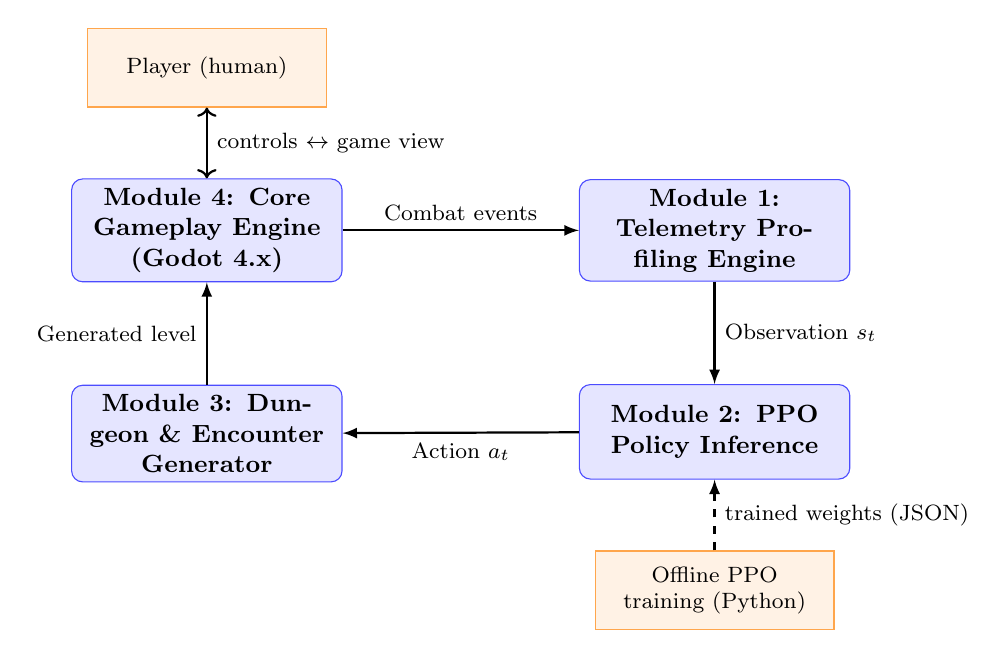
\begin{tikzpicture}[node distance=1.5cm, auto,
    block/.style={rectangle, draw=blue!70, fill=blue!10, rounded corners, text width=3.2cm, text centered, minimum height=1.2cm, font=\small\bfseries},
    data/.style={rectangle, draw=orange!70, fill=orange!10, text width=2.8cm, text centered, minimum height=1.0cm, font=\footnotesize},
    line/.style={draw, -latex, thick}]
    
    \node [block] (game) {Module 4: Core Gameplay Engine (Godot 4.x)};
    \node [block, right=3.0cm of game] (telem) {Module 1: Telemetry Profiling Engine};
    \node [block, below=1.3cm of telem] (rl) {Module 2: PPO Policy Inference};
    \node [block, below=1.3cm of game] (dungeon) {Module 3: Dungeon \& Encounter Generator};
    \node [data, above=0.9cm of game] (player) {Player (human)};
    \node [data, below=0.9cm of rl] (offline) {Offline PPO training (Python)};

    \path [line, <->] (player) -- node [right, font=\footnotesize] {controls $\leftrightarrow$ game view} (game);
    \path [line] (game) -- node [above, font=\footnotesize] {Combat events} (telem);
    \path [line] (telem) -- node [right, font=\footnotesize] {Observation $s_t$} (rl);
    \path [line] (rl) -- node [below, font=\footnotesize] {Action $a_t$} (dungeon);
    \path [line] (dungeon) -- node [left, font=\footnotesize] {Generated level} (game);
    \path [line, dashed] (offline) -- node [right, font=\footnotesize] {trained weights (JSON)} (rl);
\end{tikzpicture}
\caption{High-Level Modular Interaction Flow of Project FORGE}
\label{fig:modular_arch}
\end{figure}

\section{Stakeholders and User Classes}
The primary stakeholders and user classes interacting with FORGE are summarized in Table~\ref{tab:stakeholders}.

\begin{table}[!htbp]
\centering
\caption{Stakeholders and User Classification}
\label{tab:stakeholders}
\small
\begin{tabular}{p{0.22\textwidth}p{0.35\textwidth}p{0.35\textwidth}}
\toprule
\textbf{User Class / Stakeholder} & \textbf{Characteristics \& Needs} & \textbf{System Interaction Points} \\
\midrule
\textbf{End-User Player} & Casual or enthusiast action roguelike gamers seeking engaging, personalized challenge without tedious setup. & Gameplay controls (WASD, Mouse Sword Attack, Spacebar Dash), HUD, room traversal. \\
\textbf{Game Balance Designer} & Evaluators requiring transparency into how AI difficulty parameters adjust relative to telemetry. & Real-time Defense Overlay, parameter manual sliders, telemetry export logs. \\
\textbf{Academic Researchers} & Investigators evaluating PCGRL adaptability, solvability, and psychometric flow alignment. & Offline training scripts, policy weights JSON, automated headless CI test reports. \\
\textbf{Supervisory Panel} & Evaluators assessing project progress, code ownership, engineering rigor, and rubric compliance. & Form 2 Live Demonstration, Form 3 Written Mid-Report, Git commit evidence. \\
\bottomrule
\end{tabular}
\end{table}

\section{Success Criteria}
To provide objective benchmarks for project evaluation, the success criteria listed in Table~\ref{tab:success_criteria} were baselined.

\begin{table}[!htbp]
\centering
\caption{Measurable Project Success Criteria}
\label{tab:success_criteria}
\small
\begin{tabular}{p{0.1\textwidth}p{0.32\textwidth}p{0.25\textwidth}p{0.23\textwidth}}
\toprule
\textbf{ID} & \textbf{Success Metric} & \textbf{Target Threshold} & \textbf{Mid-1 Status} \\
\midrule
SC-01 & Topological Solvability Rate & $100\%$ across random seeds & Verified (500/500 seeds) \\
SC-02 & In-Engine Neural Inference Latency & $<1.0$\,ms per invocation & Verified (mean $0.21$\,ms, max $0.36$\,ms) \\
SC-03 & Frame Rate Stability & $\ge 60$\,FPS at the $1280\times720$ project resolution & Verified (60\,FPS constant) \\
SC-04 & Cold-Start Calibration Stability & Stable $CR_0 \in [10, 95]$ in 5 floors & Verified via $\vec{w}$ aggregation \\
SC-05 & System Fault Tolerance & Zero crash on missing weights & Verified (Heuristic fallback) \\
SC-06 & Automated CI Solvability Pass Rate & $100\%$ build pass on GitHub Actions & Verified via Headless Godot CI \\
SC-07 & Difficulty Error Rate ($\text{DER}$) & $\text{DER} \le 0.15$ against target pace & Targeted for Gate 3 Exit \\
SC-08 & Psychometric Flow Elevation & Statistically significant GEQ gain & Scheduled for FYP-2 UAT \\
\bottomrule
\end{tabular}
\end{table}

\section{Constraints and Assumptions}
\subsection*{Technical Constraints}
\begin{itemize}
    \item \textbf{Engine Constraints:} Development is confined to the Godot Engine 4.x: CI targets 4.3, and the prototype is also developed and benchmarked locally on 4.7.2. In-game forward passes must be coded in native GDScript to prevent external library or DLL installation failures on end-user machines.
    \item \textbf{Execution Budget:} Total frame compute time must not exceed $16.6$\,ms to maintain 60\,FPS vertical sync on standard hardware (Intel Core i5 / GTX 1060 equivalent).
    \item \textbf{Offline Training Horizon:} Policy training is constrained to CPU/GPU environments running Python 3.10 or newer (CI uses 3.12) with PyTorch and Stable-Baselines3.
\end{itemize}

\subsection*{Operational Assumptions}
\begin{itemize}
    \item Players interact using standard keyboard and mouse peripherals.
    \item Single-player execution without concurrent cloud dependency.
    \item Player performance changes gradually across floors, with sudden skill deviations limited in effect by the hard bounds on every difficulty parameter.
\end{itemize}

\section{Ethical, Legal and DEI Considerations}
\subsection*{Data Privacy and Player Governance}
Dynamic difficulty adaptation systems routinely raise ethical concerns regarding non-consensual biometric tracking and behavioral profiling. Project FORGE enforces a strict \textbf{Privacy-by-Design} protocol:
\begin{itemize}
    \item \textbf{Zero PII Collection:} Telemetry logs contain exclusively abstracted game mechanics data (timestamps, hit counts, health deltas). No IP addresses, device serials, or personal identifiers are captured.
    \item \textbf{Client-Side Local Storage:} Telemetry data is saved locally to user-accessible JSON files (\texttt{user://session\_telemetry.json}). No external telemetry beaconing or cloud analytics tracking is implemented.
\end{itemize}

\subsection*{Game Addiction and Dark Pattern Safeguards}
Commercial engagement-driven DDA often employs predatory algorithms designed to artificially induce near-miss scenarios to maximize monetization or daily active time. FORGE explicitly rejects dark patterns: difficulty adaptation is oriented purely toward sustaining Csikszentmihalyi's flow channel for intrinsic player satisfaction, without manipulative churn mechanics or artificial loot throttling.

\subsection*{Diversity, Equity, and Inclusion (DEI)}
By calibrating combat difficulty to individual motor abilities, FORGE inherently enhances gameplay accessibility. Novice players or players with motor impairments are accommodated without experiencing repeated, punitive failure walls, while expert players encounter escalating challenges. Visual indicators (such as glowing yellow telegraph rings on Pyromancer fireballs) ensure tactical clarity for players with varying reaction times.

\chapter{Research and Existing Solutions}
\label{chap:research}

\section{Research Method and Literature Survey Approach}
To establish a rigorous theoretical foundation and address the FYP Committee's mandate regarding state-of-the-art Dynamic Difficulty Adjustment (DDA) and Procedural Content Generation via Reinforcement Learning (PCGRL), the project team conducted a systematic literature review covering \textbf{32 sources} (peer-reviewed publications, preprints and foundational benchmarks) across premier game AI, human-computer interaction, and machine learning venues (IEEE Transactions on Games, IEEE Conference on Games, ACM CHI, Foundations of Digital Games, and Springer Multimedia Tools and Applications).

Our investigation followed a structured three-tier review methodology:
\begin{enumerate}
    \item \textbf{Generational DDA Survey:} Examining the evolution of difficulty adjustment algorithms from heuristic threshold triggers to modern statistical, continuous, and personalized reinforcement learning models~\cite{mortazavi2024dda, zohaib2018dynamic, fisher2024exploring, pfau2020enemy, fuchs2024personalized}.
    \item \textbf{PCGRL State-of-the-Art Analysis:} Reviewing learned procedural generators conditioned on target features, open-ended environments, multi-objective Pareto optimization, GPU-accelerated environments, and graph topologies~\cite{khalifa2020pcgrl, earle2021illuminating, earle2021controllable, yuan2026mopcgrl, li2025measuring, bazzaz2026imitation, earle2024pcgrlplus, rupp2024gpcgrl, yannakakis2018ai}.
    \item \textbf{Human-Centered Psychometric Instruments:} Evaluating standardized psychological scales designed to measure player flow, immersion, perceived competence, and autonomy in real-time gaming environments~\cite{denisova2016convergence, tyack2020sdt, michailidis2018flow}.
\end{enumerate}

\section{Existing Solutions and Products}
The academic and commercial landscape of adaptive content generation is categorized into three distinct evolutionary paradigms, summarized below.

\subsection{Generation 1: Heuristic and Rule-Based Systems (1990s--2000s)}
Early commercial difficulty adaptation relied on deterministic conditional triggers ($\text{IF}/\text{THEN}$ rules) operating on scalar difficulty ranks. Notable examples include:
\begin{itemize}
    \item \textbf{Resident Evil 4 (Capcom):} Implements a hidden 1--10 ``Dynamic Rank'' variable. Headshots and rapid kills increment the rank, while taking damage or dying decrements it. The rank scales adversary health and reaction speeds linearly.
    \item \textbf{Left 4 Dead (Valve):} Features the ``AI Director''~\cite{zohaib2018dynamic, mortazavi2024dda}, which monitors player stress levels (computed from health and zombie proximity) to cycle through Build-Up, Peak, and Relax phases.
    \item \textbf{Hades (Supergiant Games):} Employs an optional ``God Mode'' providing a flat $+20\%$ damage resistance upon activation, incrementing by $+2\%$ on every subsequent run death.
\end{itemize}
\textbf{Limitation:} These systems operate via scalar multipliers, suffer from high transparency, and frequently trigger the ``rubber-banding penalty,'' wherein players feel patronized upon discovering that their struggles artificially weaken enemies.

\subsection{Generation 2: Statistical and Probabilistic Modeling (2010s)}
To mitigate the rigidity of rule-based triggers, second-generation systems incorporated probabilistic inference, Markov Decision Processes (MDPs), and fuzzy logic controllers:
\begin{itemize}
    \item \textbf{Fuzzy-Logic Difficulty Controllers:} Chrysafiadi et al.~\cite{chrysafiadi2023fuzzy} designed a fuzzy-logic controller for an educational 3D game that maps imprecise descriptors of player performance onto graded difficulty adjustments.
    \item \textbf{Dynamic Elo Matchmaking:} Matchmaking algorithms adapted from chess to predict win probabilities and modulate spawn counts accordingly.
\end{itemize}
\textbf{Limitation:} While smoother than Generation 1, statistical models lack the temporal credit assignment needed to anticipate multi-room player fatigue across extended roguelike runs.

\subsection{Generation 3: Deep Reinforcement Learning (SOTA / 2020s)}
Modern research frames game generation and difficulty adaptation as reinforcement learning problems:
\begin{itemize}
    \item \textbf{PCGRL Benchmark (Khalifa et al.~\cite{khalifa2020pcgrl}):} Formulates level generation as an MDP where an agent acts as an iterative brush placing tiles to maximize path length and reachability.
    \item \textbf{Controllable Content Generators (Earle et al.~\cite{earle2021controllable}):} Conditions PCGRL generators on designer-specified numerical control targets (e.g., target path length).
    \item \textbf{Quality-Diversity and Multi-Objective PCGRL (Earle et al.~\cite{earle2021illuminating}; Yuan et al.~\cite{yuan2026mopcgrl}):} Extend learned generators to diverse level archives and to multiple simultaneous objectives (Pareto trade-offs), the latter being directly relevant to FORGE's competing goals of challenge, solvability and frame budget. Li et al.~\cite{li2025measuring} survey metrics for measuring the diversity of generated scenarios, and Bazzaz and Cooper~\cite{bazzaz2026imitation} show that players' enjoyment ratings of generated levels depend on whether they believe a human or an AI created them.
    \item \textbf{PCGRL+ Scaled Level Generators (Earle et al.~\cite{earle2024pcgrlplus}):} Demonstrates billion-step parallel level generation on GPUs, overcoming long-standing training bottlenecks in reinforcement learning procedural level generators.
    \item \textbf{Graph-Based PCGRL (Rupp \& Eckert~\cite{rupp2024gpcgrl}):} Extends PCGRL beyond 2D tile matrices to graph data (e.g., game economies and skill trees) by editing a graph's adjacency matrix, a representation that could in principle also describe room adjacency and progression graphs.
    \item \textbf{Encounter Generation for DDA (Romeo \& Bagdanov~\cite{romeo2025ntrl}):} Proposes NTRL (2025), which generates tabletop role-playing combat encounters from the real-time attributes of the party, framed as a contextual bandit, to hit a high (about 70\%) win-rate target.
    \item \textbf{Personalized Imitation-RL DDA (Fuchs et al.~\cite{fuchs2024personalized}):} Trains one agent to imitate the individual player and a second agent to defeat that imitation, personalizing opponent difficulty in a fighting-game setting.
    \item \textbf{Continuous Difficulty-Space DDA (Rahim et al.~\cite{rahim2023continuous}):} Replaces the small discrete state--action spaces of earlier RL-based DDA with a continuous difficulty metric in a visual working-memory game, reporting better competence ratings and a smaller score decline over a session than rule-based baselines in a 52-participant study.
    \item \textbf{Long-Term Adaptation Effects (Pfau et al.~\cite{pfau2020enemy}):} Reports a long-term study in a live MMORPG in which deep player-behavior models for DDA improved intrinsic motivation compared with heuristic parameter tuning, whose adjustments players often notice (e.g., rubber-banding).
    \item \textbf{Industrial Engagement Optimization (Xue et al.~\cite{xue2017dynamic}):} Formulates DDA for a commercial game as an optimization problem that selects difficulty to maximize player engagement (session length and retention).
    \item \textbf{DDA Methods Comparison (Fisher \& Kulshreshth~\cite{fisher2024exploring}):} Compares five performance-based, emotion-based and hybrid adjustment strategies in a custom first-person shooter within-subjects study, finding no single method that clearly beat static difficulty, which underlines the difficulty of tuning adaptation well.
\end{itemize}

\section{Comparison of Existing Solutions}
Table~\ref{tab:lit_comparison} evaluates Project FORGE against representative systems from both commercial gaming and peer-reviewed literature.

\begin{table}[!htbp]
\centering
\caption{Systematic Comparison of Game Difficulty Adjustment and PCG Paradigms}
\label{tab:lit_comparison}
\scriptsize
\begin{tabular}{p{0.20\textwidth}p{0.14\textwidth}p{0.14\textwidth}p{0.13\textwidth}p{0.12\textwidth}p{0.13\textwidth}}
\toprule
\textbf{System / Reference} & \textbf{Paradigm} & \textbf{Adaptation Loop} & \textbf{Action Space} & \textbf{Solvability Proof} & \textbf{In-Engine Overhead} \\
\midrule
\textit{Resident Evil 4} & Gen 1 Heuristic & Reactive scalar rank & Scalar health/dmg & Fixed design & Negligible \\
\textit{Left 4 Dead} AI Director~\cite{zohaib2018dynamic} & Gen 1 Heuristic & Pacing state machine & Spawn wave timer & Fixed design & Low \\
Fuzzy DDA~\cite{chrysafiadi2023fuzzy} & Gen 2 Statistical & Reactive fuzzy rules & Graded multipliers & Fixed design & Low \\
\texttt{gym-pcgrl}~\cite{khalifa2020pcgrl} & Gen 3 RL & Open-loop target & Discrete tile grid & Heuristic reward & High (Python env) \\
Controllable PCGRL~\cite{earle2021controllable} & Gen 3 RL & Open-loop designer & Scalar target vector & Path-length reward & High (External) \\
NTRL~\cite{romeo2025ntrl} & Gen 3 RL & Party-state bandit & Encounter composition & N/A (tabletop) & Not reported \\
\textbf{FORGE (Ours)} & \textbf{Gen 3 RL + DDA} & \textbf{Closed-loop telemetry} & \textbf{Continuous 7D ($\vec{E}, \vec{M}$)} & \textbf{Connected by construction (BFS-verified)} & \textbf{Zero ($\approx 0.2$\,ms GDScript)} \\
\bottomrule
\end{tabular}
\end{table}

\section{Limitations and Gaps in Existing Literature}
Our literature review isolates three critical scientific and architectural gaps:
\begin{enumerate}
    \item \textbf{The Closed-Loop Personalization Void:} Prevailing PCGRL algorithms generate layouts conditioned either on random seeds or on explicit, designer-crafted target constraints~\cite{earle2021controllable, earle2024pcgrlplus}, rather than from a model of the individual player's experience as advocated by experience-driven PCG~\cite{yannakakis2011experience}. Furthermore, while foundational literature surveys evaluate the recent rise of Large Language Models (LLMs) for high-level creative game design~\cite{gallotta2024llmsurvey}, LLMs lack sub-millisecond real-time predictability for runtime combat modulation. No literature framework connects continuous, unprompted player behavioral profiling directly into an active, multi-attribute procedural generator.
    \item \textbf{The Scalar Combat Balancing Oversimplification:} Most DDA systems reduce difficulty to a one-dimensional multiplier (e.g., enemy health $+10\%$). Real combat difficulty is fundamentally combinatorial: a high-speed adversary with low health requires quick reflexes, whereas a slow, heavily armored adversary requires spatial kiting. Existing systems fail to navigate this multi-attribute trade-off.
    \item \textbf{The Sim-to-Real Deployment Gap:} Benchmark PCGRL systems rely on external Python runtimes, Torch environments, or heavy socket connections that introduce unacceptable latency and deployment hurdles for commercial standalone games.
\end{enumerate}

\section{Proposed Solution: The FORGE Architecture}\label{sec:proposed}
FORGE directly addresses these limitations through a \textbf{Two-Stage Decoupled System Architecture}:
\begin{itemize}
    \item \textbf{Stage 1: Deterministic Spatial Topology Synthesis.} The dungeon structure is generated by a random walk with branching on a grid, where each new room is attached to an existing room through a matching door pair. The resulting room graph is connected by construction, so the exit room is always reachable from the start room; the CI harness confirms this with a breadth-first search over the door graph on 500 seeds.
    \item \textbf{Stage 2: Closed-Loop PPO Combat Ecology.} A Proximal Policy Optimization agent observes a normalized 8-dimensional state vector ($s_t \in \mathbb{R}^8$: three player-performance signals, four current difficulty settings and run depth) and outputs a continuous 7D action vector ($a_t \in [-1, 1]^7$). This action modulates enemy physical attributes (health, damage, speed, aggro radius), hazard frequency, and room density.
    \item \textbf{Zero-Dependency Embedded Inference:} The trained policy weights are exported from PyTorch to a compact JSON file. At runtime, an optimized matrix multiplication engine in native GDScript executes the neural forward pass in about $0.2$\,ms (measured), guaranteeing client-side platform portability with zero external dependencies.
\end{itemize}

\section{Complex Computing Problem (CCP) Justification}
Under the FAST-NUCES and Washington Accord engineering criteria, Project FORGE qualifies as a \textbf{Complex Computing Problem (CCP)} across multiple dimensions:
\begin{itemize}
    \item \textbf{WP-1 (In-depth Computing Knowledge):} Integrates advanced reinforcement learning (PPO clipped surrogate optimization), state-space observation modeling, procedural level synthesis algorithms, and real-time game engine physics.
    \item \textbf{WP-2 (Conflicting Requirements \& Multi-Objective Trade-offs):} The generator must simultaneously balance competing objectives: maintaining player challenge within the flow channel, guaranteeing topological solvability, avoiding repetitive level layouts, and maintaining a strict $16.6$\,ms (60\,FPS) rendering frame budget.
    \item \textbf{WP-3 (Non-Trivial Mathematical \& Analytical Formulation):} Involves non-linear observation-action mappings, non-uniform difficulty-weighted temporal aggregation ($\sum w_i S_i$), matrix algebra for forward propagation in GDScript, and clipped policy gradient bounds.
    \item \textbf{WP-4 (Infrequent \& Novel Problems):} Formulates real-time sim-to-real transfer of offline RL policies into a lightweight client-side game engine without external Python/ONNX runtimes.
    \item \textbf{WP-5 (Engineering Integration):} Bridges offline deep RL training frameworks (Stable-Baselines3, PyTorch, Gymnasium) with real-time 2D game architecture (Godot 4.x).
    \item \textbf{WP-6 (Significance of Non-Functional Constraints):} Strict latency bounds ($<1.0$\,ms inference), zero-crash reliability under missing weights, and client-side privacy governance.
\end{itemize}

\section{Technical Challenges Anticipated and Encountered}
During design and initial implementation, the team encountered and resolved three major technical hurdles:
\begin{enumerate}
    \item \textbf{Sim-to-Real Transfer and Player Modeling:} In offline training, real human playtesters cannot provide the millions of frames required by PPO. We engineered a stochastic simulated player whose skill drifts smoothly and whose clearing time is a function of room difficulty, drawing on automated playtesting for parameter tuning, curiosity-conditioned trajectories, and procedural personas~\cite{holmgard2019procedural, zook2014playtesting, sestini2024automated}.
    \item \textbf{Reward Hacking During Offline Policy Training:} In the first version of the reward, completion time was compared with a fixed total-time target. Because total time equals room count times time per room, the PPO agent could satisfy the target by pinning the room count at an extreme without adjusting any combat parameter. We resolved this by judging pace per room and adding a penalty for room counts that do not track the combat challenge (Equation~\ref{eq:reward_function}).
    \item \textbf{Difficulty Thrashing and Player Frustration:} Sudden spikes in player clearing time could cause an unconstrained policy to swing wildly between extreme difficulty tiers. We mitigate this with PPO's clipped objective during training, hard bounds on every output parameter (Table~\ref{tab:param_ranges}) and the cold-start anchor. The runtime does not yet include an explicit inter-floor rate limiter, and the shipped policy can move parameters by a large fraction of their range in a single step (Section~\ref{sec:policy_eval}); a limiter is planned for FYP-2.
\end{enumerate}

\section{Research Findings and Core Design Decisions}

\subsection{Why PPO Over SAC, DQN, and Contextual Bandits?}
A core inquiry raised during the Proposal Defense was the theoretical justification for selecting PPO over alternative reinforcement learning paradigms. Table~\ref{tab:rl_comparison} details this algorithmic trade-off.

\begin{table}[!htbp]
\centering
\caption{Algorithmic Comparison: Justifying PPO for Dynamic Difficulty Adjustment}
\label{tab:rl_comparison}
\small
\begin{tabular}{p{0.18\textwidth}p{0.2\textwidth}p{0.27\textwidth}p{0.25\textwidth}}
\toprule
\textbf{Algorithm} & \textbf{Action Space} & \textbf{Sample / Stability Profile} & \textbf{Suitability for DDA} \\
\midrule
\textbf{DQN}~\cite{mnih2015human} & Discrete Only & High sample efficiency; prone to Q-value overestimation & Poor: Discretizing 7 continuous parameters leads to curse of dimensionality. \\
\textbf{Contextual Bandits} & Discrete/Continuous & Myopic single-step; cannot model multi-room credit assignment & Poor: Ignores long-term fatigue across multi-floor dungeon runs. \\
\textbf{SAC}~\cite{haarnoja2018soft} & Continuous & Off-policy; highly sample efficient but prone to hyperparameter volatility & Moderate: Maximum entropy can produce aggressive difficulty swings. \\
\textbf{PPO (Ours)}~\cite{schulman2017proximal} & Continuous & On-policy; monotonic policy improvement via clipped surrogate objective & \textbf{Exemplary:} Clipped objective acts as an intrinsic skill shock-absorber. \\
\bottomrule
\end{tabular}
\end{table}

\subsection{Mathematical Proof: PPO Clipped Objective as a Skill Shock-Absorber}\label{sec:ppo_proof}
The core vulnerability in online difficulty adjustment is the occurrence of sudden player skill shocks (e.g., an expert player dying due to an accidental trap trigger, or a novice speedrunning through a sparsely populated room). In unconstrained actor-critic frameworks, such extreme gradient signals cause catastrophic policy shifts, inducing severe difficulty thrashing.

PPO resolves this by optimizing the clipped surrogate objective function:
\begin{equation}
L^{CLIP}(\theta) = \hat{\mathbb{E}}_t \left[ \min\left(r_t(\theta)\hat{A}_t, \, \text{clip}\left(r_t(\theta), \, 1-\epsilon, \, 1+\epsilon\right)\hat{A}_t\right) \right]
\label{eq:ppo_clip}
\end{equation}
where $r_t(\theta) = \frac{\pi_\theta(a_t | s_t)}{\pi_{\theta_{old}}(a_t | s_t)}$ represents the probability ratio of the proposed action under the updated versus previous policy, $\hat{A}_t$ is the estimated advantage function, and $\epsilon \approx 0.2$ is the clipping boundary.

Because the policy ratio $r_t(\theta)$ is strictly constrained within the interval $[1-\epsilon, 1+\epsilon]$, the gradient update is bounded. Even when an abrupt change in player performance generates an enormous advantage signal $\hat{A}_t$, the maximum update per iteration is bounded by $\epsilon$. Consequently, PPO's trust region keeps each \emph{training} update small and makes learning robust to noisy or extreme episodes. At deployment the actor is a fixed network, so how smoothly difficulty evolves across floors depends on the learned mapping and on the hard output bounds; we therefore measure it (Section~\ref{sec:policy_eval}) instead of assuming it.

\subsection{Preserving the Principle of Change Blindness}
In game psychology, ``change blindness'' refers to the human inability to detect gradual, continuous alterations in visual or environmental features~\cite{simons2005change}. The design goal is that difficulty parameters ($\vec{E}, \vec{M}$) change gradually between floors so that players do not notice the intervention; the current prototype bounds them to fixed ranges, and an explicit per-floor rate limiter that enforces gradual change is scheduled for FYP-2. They experience the game as an intrinsically fair, consistently challenging world, preserving their feelings of competence and self-efficacy~\cite{tyack2020sdt}.

\chapter{Proposal Feedback and Iteration Plan}
\label{chap:plan}

\section{Proposal Feedback Summary}
Project FORGE was defended at the FYP Proposal Defense I before the Evaluation Committee of the FAST School of Computing, FAST-NUCES, Islamabad. The committee officially issued the following verdict:
\begin{quote}
\textbf{Decision:} \textit{Approved with Minor Modifications (Project Code: F26-012-FORGE)}\\
\textbf{Committee Summary:} \textit{``Good project. Good presentation and demonstration. Demonstrates satisfactory understanding of the project concepts and approach. The game's aesthetics should be improved. They should study related literature review deeply as the game is based on research... Extend the literature review to comprehensively cover Dynamic Difficulty Adjustment (DDA)... Strengthen the technical justification for PPO... Define and validate the judge model using empirical player data... Clearly distinguish procedural level generation from difficulty adaptation... Specify measurable acceptance criteria... Document risks, fallback strategies, and ethical considerations.''}
\end{quote}

Rather than treating these modifications as superficial corrections, the project team treated the committee's feedback as a binding technical contract that reshaped our development roadmap across Iterations 1 and 2.

\section{Proposal Action Register}
Table~\ref{tab:action_register} documents the complete Proposal Action Register, mapping every committee directive to the specific engineering action taken, its implementation status, and its location in the project documentation and codebase.

\begin{table}[!htbp]
\centering
\caption{Proposal Feedback Resolution Action Register}
\label{tab:action_register}
\scriptsize
\begin{tabular}{p{0.04\textwidth}p{0.22\textwidth}p{0.32\textwidth}p{0.12\textwidth}p{0.22\textwidth}}
\toprule
\textbf{No.} & \textbf{Directive / Required Change} & \textbf{Action Taken in Iteration 1 \& 2} & \textbf{Status} & \textbf{Evidence} \\
\midrule
1 & Improve game aesthetics (sprites, juice, feedback). & Replaced procedural vector circles with custom 2D pixel-art sprites; integrated trauma camera shake, floating damage text, and Cinzel/Inter typography. & Completed & Chapter~\ref{chap:iter1}, §\ref{sec:iter1_features}; Figs. in App.~\ref{app:diagrams} \\
\midrule
2 & Variety of attacks for enemy and player powers. & Developed Ranged Pyromancer with telegraphed fireball projectile and retreat AI; implemented player dodge roll with invulnerability frames and cooldown. & Completed & \texttt{Enemy.gd}, \texttt{Player.gd}, \texttt{ProjectileFireball.gd} \\
\midrule
3 & Engaging, playable game experience without AI. & Engineered a ``Static Roguelike Baseline'' mode toggle in Defense Overlay scaling difficulty deterministically by $+8\%$ per floor. & Completed & \texttt{DefenseOverlay.gd}, Chapter~\ref{chap:iter1} \\
\midrule
4 & Clarify project scope boundaries (in-scope vs. out). & Formulated a strict three-tier Scope Boundary Matrix defining Mid-1 commitments, Final-1/FYP-2 deliverables, and out-of-scope items. & Completed & Table~\ref{tab:scope_matrix}, §\ref{sec:scope} \\
\midrule
5 & Clear, measurable evaluation criteria for RL and game. & Formulated 8 quantitative success metrics (solvability, latency, DER, $CR_0$ convergence) and standardized psychometrics (GEQ, PENS). & Completed & Table~\ref{tab:success_criteria}, Chapter~\ref{chap:testing} \\
\midrule
6 & Comprehensive DDA literature review. & Conducted systematic survey of 32 sources; classified DDA into 3 generational paradigms; synthesized flow and engagement literature. & Completed & Chapter~\ref{chap:research}, Table~\ref{tab:lit_comparison} \\
\midrule
7 & Strengthen technical justification for PPO vs. alternatives. & Compared PPO with SAC, DQN, and Bandits; mathematically formulated clipped surrogate objective as an intrinsic skill shock-absorber. & Completed & Section~\ref{sec:ppo_proof}, Table~\ref{tab:rl_comparison} \\
\midrule
8 & Define and validate judge model empirically. & Maintained linear proxy for Mid-1; scheduled the offline supervised Gradient Boosted Regressor with TreeSHAP and a 25-session empirical corpus for FYP-1 Final (Gate 3 Exit, Weeks 11--14). & Scheduled for Final-1 & Section~\ref{sec:domain}, Chapter~\ref{chap:fyp2} \\
\midrule
9 & Distinguish procedural level generation from DDA. & Formally decoupled architecture into Stage 1 (Connected Spatial Topology, BFS-verified in CI) and Stage 2 (Closed-Loop PPO Combat Adapter). & Completed & Section~\ref{sec:proposed}, Chapter~\ref{chap:design} \\
\midrule
10 & Document risks, fallbacks, and telemetry ethics. & Developed zero-crash heuristic fallback in GDScript; implemented client-side zero-PII local data governance; formulated risk register. & Completed & Section~\ref{sec:ethics}, Section~\ref{sec:risk} \\
\bottomrule
\end{tabular}
\end{table}

\section{Iterative Development Strategy}
Project FORGE follows an Agile iterative lifecycle structured into five formal evaluation gates across two academic semesters:
\begin{itemize}
    \item \textbf{Gate 1 (Inception \& Technical Spike — Weeks 1--6):} Verified feasibility of training a PPO policy in Python and running an MLP forward pass in pure GDScript.
    \item \textbf{Gate 2 (Requirements \& SRS Elaboration — Weeks 7--8):} Formalized testable functional and non-functional specifications; baselined cold-start calibration mathematics.
    \item \textbf{Gate 3 (Architecture Baseline \& Mid-1 Evaluation — Weeks 9--10):} Integrated visual aesthetics, ranged combat behaviors, static baseline mode, and automated headless CI solvability testing.
    \item \textbf{Gate 4 (System Integration \& Mid-2 Evaluation — Weeks 11--26):} Full 5-archetype ecosystem, empirical Judge model, and TreeSHAP explainability engine (delivered at FYP-1 Final, Weeks 11--14), followed by the equipment shop economy, system integration and performance benchmarking through Week 26.
    \item \textbf{Gate 5 (Production Acceptance \& Final-2 Evaluation — Weeks 27--32):} 10-participant human UAT study, psychometric evaluation, and public release distribution.
\end{itemize}

\section{Iteration 1 Plan (Weeks 1--6 / Proposal \& POC Spike)}
The primary objective of Iteration 1 was de-risking the fundamental technical hypothesis: can an RL policy trained offline control difficulty parameters inside Godot?
\begin{itemize}
    \item \textbf{Deliverables:} Godot 4.x prototype with rudimentary geometric shapes (white circle player, red circle enemy), basic sword slash, flat 3-room layout, preliminary \texttt{train\_ppo\_difficulty.py} script exporting JSON weights, and basic telemetry recording.
    \item \textbf{Outcome:} Confirmed that pure-GDScript matrix math could execute forward passes without relying on external Python or ONNX runtimes.
\end{itemize}

\section{Iteration 2 Plan (Weeks 7--10 / Mid-1 Evaluation Sprint)}
Iteration 2 focused directly on fulfilling the committee's mandate and preparing the production-grade Mid-1 deliverable:
\begin{itemize}
    \item \textbf{Objectives:} Elevate game aesthetics to commercial standards; introduce enemy attack variety; implement the cold-start calibration protocol; engineer a static roguelike baseline; establish an automated CI pipeline.
    \item \textbf{Delivered Features:}
    \begin{enumerate}
        \item Integrated 2D pixel-art sprites, camera trauma shake (decay rate $3.6$\,s$^{-1}$), and floating combat text.
        \item Created Ranged Pyromancer with retreat AI and telegraphed fireball projectiles; added player dodge roll ($0.2$\,s dash with invulnerability).
        \item Implemented 5-Floor Cold-Start Protocol with weighted $CR_0$ baseline aggregation ($\vec{w} = [1.0, 1.5, 2.0, 2.5, 3.0]$).
        \item Added Static Roguelike Baseline mode toggle in the live Defense Telemetry Overlay.
        \item Built GitHub Actions CI pipeline executing headless Godot 4.3 solvability simulations across 500 seeds.
        \item Compiled formal SRS and SDS engineering specifications.
    \end{enumerate}
\end{itemize}

\section{Work Breakdown and Responsibilities}
Table~\ref{tab:wbs} details the individual technical ownership and task allocation among the three team members.

\begin{table}[!htbp]
\centering
\caption{Team Member Technical Responsibility Allocation Matrix}
\label{tab:wbs}
\small
\begin{tabular}{p{0.25\textwidth}p{0.25\textwidth}p{0.42\textwidth}}
\toprule
\textbf{Team Member} & \textbf{Primary Role} & \textbf{Core Module Ownership \& Tasks} \\
\midrule
\textbf{Rayan Ahmed}\newline (23i-0018) & Engine Architecture \& Gameplay Lead & Godot engine framework, player combat mechanics, dodge roll iframes, enemy finite state machines (Melee \& Ranged), projectile kinematics, visual juice (camera shake, damage floaters), sprite pipeline. \\
\midrule
\textbf{Rana Raza Ahmed}\newline (23i-0060) & Machine Learning \& PCG Lead & Offline Gymnasium environment, PPO reward formulation, policy weight serialization, in-engine GDScript forward pass (\texttt{PPOPolicy.gd}), cold-start $CR_0$ mathematical formulation. \\
\midrule
\textbf{Uwaid Munir}\newline (23i-2574) & Telemetry Analytics \& Evaluation Lead & Telemetry logging engine (\texttt{TelemetryLogger.gd}), event capture, GitHub Actions CI/CD headless solvability test pipeline, test case authoring, verification suite, and SRS/SDS documentation. \\
\bottomrule
\end{tabular}
\end{table}

\section{Progress Against Plan}
Table~\ref{tab:milestones} presents the progress tracking against the original project schedule.

\begin{table}[!htbp]
\centering
\caption{Milestone Tracking and Schedule Progress}
\label{tab:milestones}
\small
\begin{tabular}{p{0.32\textwidth}p{0.18\textwidth}p{0.18\textwidth}p{0.18\textwidth}}
\toprule
\textbf{Milestone / Deliverable} & \textbf{Planned Date} & \textbf{Actual Date} & \textbf{Status} \\
\midrule
Proposal Defense & Week 4 & Week 4 & Completed (Approved) \\
Literature Survey & Week 6 & Week 6 & Completed (32 Sources) \\
Dungeon Sprites \& Visual Juice & Week 8 & Week 8 & Completed \\
Ranged Enemy \& Dodge Roll & Week 9 & Week 9 & Completed \\
5-Floor Cold-Start Protocol & Week 9 & Week 9 & Completed \\
Static Roguelike Baseline Mode & Week 10 & Week 10 & Completed \\
Headless CI Solvability Pipeline & Week 10 & Week 10 & Completed \\
Mid-1 Formal Report Submission & Week 10 & Week 10 & Completed (On Schedule) \\
\bottomrule
\end{tabular}
\end{table}

\section{Delays, Deviations and Recovery Plan}
During Iteration 2, two technical deviations arose, both of which were successfully resolved:
\begin{enumerate}
    \item \textbf{Deviation 1: Godot 4 Headless Export CI Template Overhead.} Running full headless game exports in GitHub Actions initially failed due to missing Windows export templates. \textbf{Recovery:} We restructured the CI workflow into a dedicated two-stage check: (1) headless Godot scene/script syntax compilation check via \texttt{--headless --quit}; and (2) headless automated solvability verification executing a lightweight test harness runner script across 500 random seeds.
    \item \textbf{Deviation 2: PPO Reward Hacking in Simulated Training.} The first reward compared the total clearing time with a fixed target, which the agent satisfied by manipulating the room count instead of combat difficulty. \textbf{Recovery:} We redesigned the reward function in \texttt{train\_ppo\_difficulty.py} to judge pace per room, add death and pacing penalties, and penalize room counts that do not track the combat challenge.
\end{enumerate}
All milestones for Mid-1 have been completed on schedule with zero debt carried into Iteration 3.

\chapter{Software Requirements Specification}
\label{chap:reqs}

\section{User Interactions and System Actors}
The FORGE system interacts with three primary classes of actors:
\begin{enumerate}
    \item \textbf{Primary Actor (Player):} Navigates the dungeon, engages in melee combat, evades enemy projectiles via dodge rolls, collects health pickups, avoids traps, and transitions through floor portals.
    \item \textbf{Secondary Actor (Game Balance Evaluator / Supervisor):} Monitors live telemetry via the Defense Overlay HUD, toggles between Adaptive PPO mode and Static Baseline mode, manually overrides difficulty parameters via sliders, and inspects exported session logs.
    \item \textbf{Automated System Actor (GitHub Actions CI Runner):} Executes automated headless test scripts, parses exit codes, and asserts topological solvability across randomized seeds.
\end{enumerate}

\section{Use Case Diagram}
Figure~\ref{fig:use_case_diagram} depicts the core use cases and actor associations within Project FORGE.

\begin{figure}[!htbp]
\centering
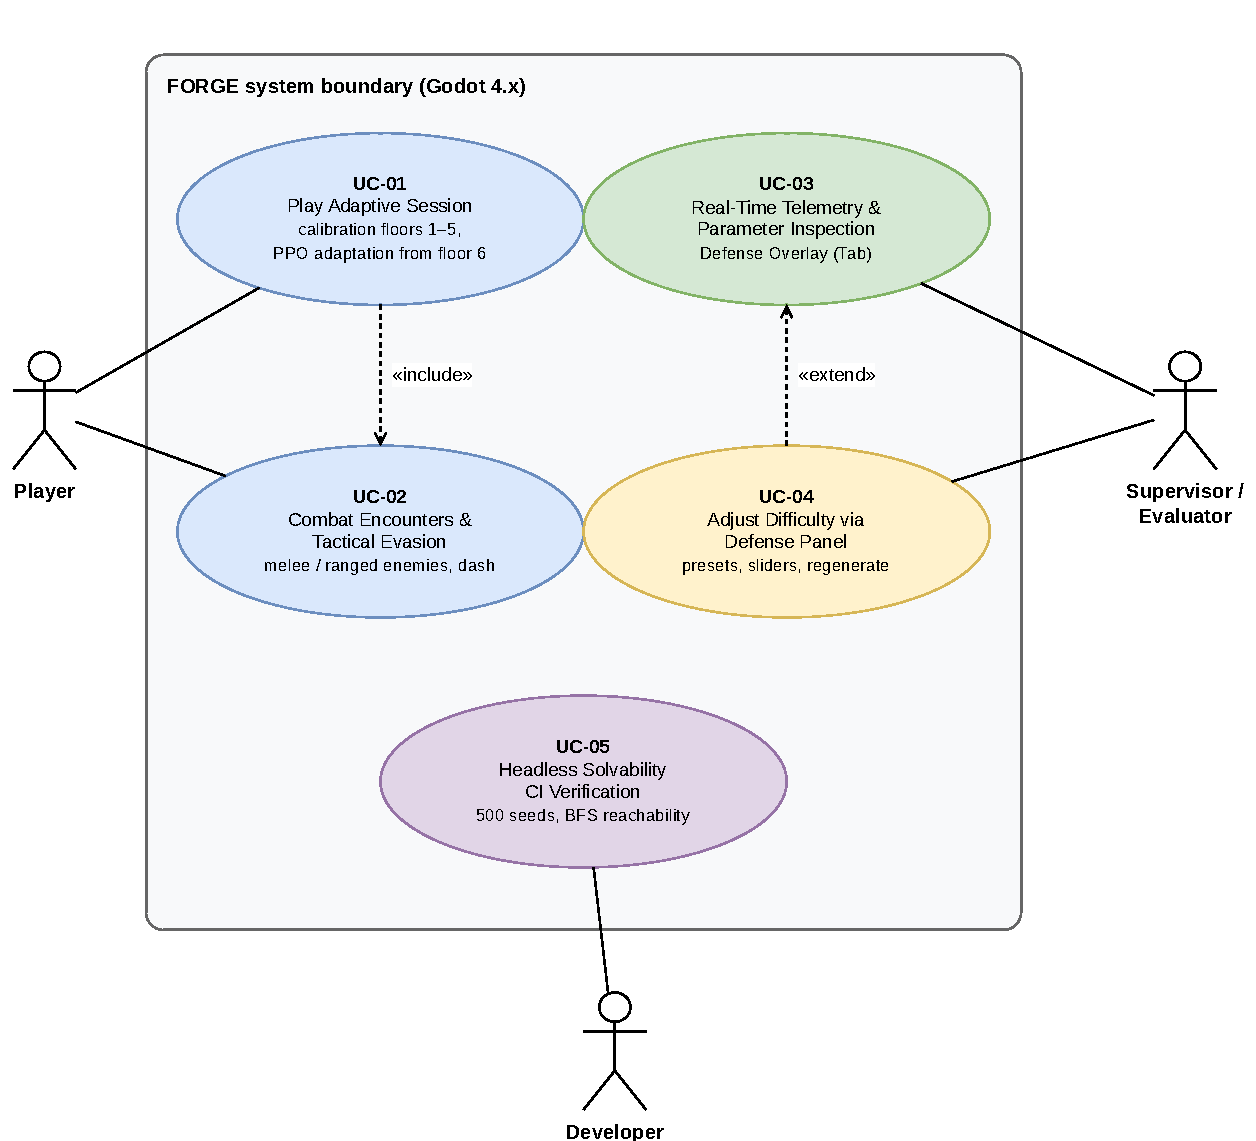
\includegraphics[width=0.95\textwidth]{ThesisFigs/fig_4_2_use_case}
\caption{Unified Use Case Diagram for Project FORGE}
\label{fig:use_case_diagram}
\end{figure}

\section{Detailed Use Cases}

\subsection{UC-01: Play Adaptive Session with Cold-Start Calibration}
\begin{itemize}
    \item \textbf{Actors:} Player (Primary), PPO Generator (System).
    \item \textbf{Preconditions:} Game is launched; player selects ``Start Game'' from the main menu; \texttt{policy\_weights.json} exists or heuristic fallback is ready.
    \item \textbf{Trigger:} Player initiates a new dungeon run.
    \item \textbf{Main Scenario:}
    \begin{enumerate}
        \item System loads Floor 1 in Cold-Start mode with baseline difficulty parameters ($\vec{E}_1, \vec{M}_1$).
        \item Player traverses rooms, defeats adversaries, and reaches the exit portal.
        \item \texttt{TelemetryLogger} records clearing time, damage ratio, and deaths.
        \item Steps 1--3 repeat through Floor 5 with escalating parameter tiers.
        \item At Floor 5 exit, system computes $CR_0 = \sum w_i \cdot \text{Score}_i / \sum w_i$ ($\vec{w} = [1.0, 1.5, 2.0, 2.5, 3.0]$).
        \item System builds the initial PPO observation $s_0$ from the same weighted calibration records, expressed on the policy's training scales (Equation~\ref{eq:s0_seed}), and predicts action $a_0$; $CR_0$ is shown to the player and evaluator as a summary.
        \item Floor 6 loads with personalized parameters; closed-loop PPO adaptation governs subsequent floors.
    \end{enumerate}
    \item \textbf{Alternative Path:} If the player dies, the death is recorded in telemetry and the player respawns in the start room of the current floor after 1.2\,s; cleared rooms stay cleared and difficulty parameters are unchanged until the floor is exited.
    \item \textbf{Postconditions:} Complete session telemetry written to \texttt{user://session\_telemetry.json}.
\end{itemize}

\subsection{UC-02: Combat Encounters and Tactical Evasion}
\begin{itemize}
    \item \textbf{Actors:} Player, Melee Crawler, Ranged Pyromancer.
    \item \textbf{Preconditions:} Player enters a non-cleared room containing active enemies.
    \item \textbf{Main Scenario:}
    \begin{enumerate}
        \item Melee Crawlers detect player within aggro radius and initiate pursuit (default $125$\,px/s, PPO-controlled).
        \item Ranged Pyromancers hold a standoff distance ($140$--$280$\,px) and initiate $0.5$\,s telegraph tell.
        \item Pyromancers launch a fireball projectile along the direction to the player at the moment the telegraph ends (no lead prediction).
        \item Player executes Spacebar dodge roll ($0.2$\,s dash), gaining $0.26$\,s of invulnerability to evade the projectile.
        \item Player delivers sword strike to enemy hitbox; system computes damage, triggers camera shake (decay rate $3.6$\,s$^{-1}$), and pops yellow floating damage text.
        \item Enemies defeated; doors unlock. Health pickups were placed when the room was generated: a combat room holds a potion with probability $1 - \text{resource scarcity}$.
    \end{enumerate}
    \item \textbf{Postconditions:} Combat damage dealt and received logged by \texttt{TelemetryLogger}.
\end{itemize}

\subsection{UC-03: Real-Time Telemetry and Defense Inspection}
\begin{itemize}
    \item \textbf{Actors:} Game Evaluator / Supervisor.
    \item \textbf{Preconditions:} Game is actively running in gameplay state.
    \item \textbf{Trigger:} Evaluator presses the \texttt{Tab} key.
    \item \textbf{Main Scenario:}
    \begin{enumerate}
        \item System renders the semi-transparent Defense Telemetry Overlay HUD.
        \item HUD displays current floor index, active mode (Adaptive vs. Static), cold-start status, and raw observation signals ($s_t$).
        \item Displays live sliders showing current enemy health, damage, speed, aggro radius, hazard density, and room count.
        \item Evaluator adjusts a slider manually; system applies the override dynamically to the current floor.
    \end{enumerate}
    \item \textbf{Postconditions:} Parameter overrides reflected in real-time enemy behavior.
\end{itemize}

\section{Functional Requirements}

\subsection{Module 1: Telemetry and Behavioral Profiling}
\begin{itemize}
    \item \textbf{FR-01 (Session Telemetry Collection):} The system shall capture room clearing duration, player damage received, damage dealt to enemies, death events, and potion pickups, logging events at 60\,FPS without frame latency.
    \item \textbf{FR-02 (Cold-Start Weighted Calibration):} The system shall enforce a 5-floor calibration sequence calculating an Initial Combat Rating ($CR_0 \in [10, 95]$) using non-uniform weights $\vec{w} = [1.0, 1.5, 2.0, 2.5, 3.0]$ across pace, survival, and damage execution.
    \item \textbf{FR-03 (JSON Telemetry Persistence):} The system shall serialize all session events to \texttt{user://session\_telemetry.json} upon floor completion and game exit.
\end{itemize}

\subsection{Module 2: Reinforcement Learning and Difficulty Policy}
\begin{itemize}
    \item \textbf{FR-04 (PPO Action Inference):} The system shall pass an 8-dimensional normalized observation vector ($s_t$) through an embedded MLP with two hidden layers in GDScript, producing a 7-dimensional continuous action vector ($a_t \in [-1, 1]^7$).
    \item \textbf{FR-05 (Heuristic Fallback Autonomy):} If \texttt{policy\_weights.json} is missing or corrupted, the system shall engage a deterministic heuristic policy that adjusts parameters from a linear performance signal (clearing time, deaths, damage taken) without raising unhandled exceptions.
\end{itemize}

\subsection{Module 3: Dungeon Layout and Encounter Synthesis}
\begin{itemize}
    \item \textbf{FR-06 (Topological Connectivity):} The system shall generate connected room layouts (every room is attached to a previously placed room through a matching door pair), and the CI harness shall verify with a breadth-first search over the door graph that the exit room is reachable from the start room.
    \item \textbf{FR-07 (Parameter Denormalization):} The system shall map normalized PPO actions ($[-1, 1]$) into bounded game engine ranges: enemy health $[20, 120]$\,HP, enemy damage $[5, 50]$, enemy speed $[60, 220]$\,px/s, aggro radius $[100, 450]$\,px, hazard density $[0.05, 0.80]$, resource scarcity $[0.10, 0.90]$, and room count $[5, 9]$.
\end{itemize}

\subsection{Module 4: Core Gameplay and Combat}
\begin{itemize}
    \item \textbf{FR-08 (Multi-Archetype Enemy Combat):} The system shall instantiate Melee Crawlers (direct path pursuit, melee slash on contact) and Ranged Pyromancers (kiting AI, telegraphed fireball projectile).
    \item \textbf{FR-09 (Player Dodge Roll):} The system shall execute an evasive dash on Spacebar input, lasting $0.2$\,s and granting $0.26$\,s of invulnerability, with a $1.0$\,s cooldown timer.
    \item \textbf{FR-10 (Static Roguelike Baseline Toggle):} The system shall provide an in-engine toggle disabling PPO adaptation and scaling enemy health and damage by a fixed $+8\%$ per floor.
\end{itemize}

\section{Non-Functional Requirements}

\subsection{Reliability and Fault Tolerance}
\begin{itemize}
    \item \textbf{NFR-01 (Zero-Crash Fallback):} The system shall gracefully degrade to the heuristic fallback policy upon missing or malformed JSON weights, maintaining continuous gameplay without crashing.
    \item \textbf{NFR-02 (Solvability Integrity):} The dungeon generator shall produce layouts in which every room is reachable from the start room, for every room count the game can request (3--9).
\end{itemize}

\subsection{Usability and Visual Polish}
\begin{itemize}
    \item \textbf{NFR-03 (Visual Feedback \& Juice):} Player and enemy damage events shall trigger trauma camera shake that settles within $0.3$\,s ($\le 1/3.6$\,s even at maximum trauma; about $0.12$\,s for a single hit) and spawn color-coded floating text numbers (yellow for enemy hit, red for player hurt, green for healing).
    \item \textbf{NFR-04 (Combat Telegraphing):} Ranged projectile attacks shall display a minimum $0.5$\,s visual tell prior to launch to allow human reaction.
\end{itemize}

\subsection{Performance and Latency}
\begin{itemize}
    \item \textbf{NFR-05 (Rendering Frame Rate):} The game engine shall maintain a stable $\ge 60$\,FPS rendering rate at the $1280\times720$ project resolution, with frame delta not exceeding $16.6$\,ms.
    \item \textbf{NFR-06 (Neural Inference Latency):} The in-engine pure-GDScript neural network forward pass shall compute action predictions with a median below $1.0$\,ms per invocation.
\end{itemize}

\subsection{Security and Data Privacy}
\begin{itemize}
    \item \textbf{NFR-07 (Privacy by Design):} The telemetry system shall collect zero Personally Identifiable Information (PII) and store all telemetry locally on the client machine without external internet transmission.
\end{itemize}

\section{Acceptance Criteria}
Table~\ref{tab:acceptance_criteria} defines the objective acceptance criteria used to verify requirements completion.

\begin{table}[!htbp]
\centering
\caption{Requirements Acceptance Criteria and Verification Protocol}
\label{tab:acceptance_criteria}
\small
\begin{tabular}{p{0.12\textwidth}p{0.32\textwidth}p{0.34\textwidth}p{0.14\textwidth}}
\toprule
\textbf{Req. ID} & \textbf{Acceptance Metric} & \textbf{Verification Protocol} & \textbf{Mid-1 Status} \\
\midrule
FR-01 & Event Capture Precision & Scripted hits (20 taken, $3\times35$ dealt) appear exactly in the snapshot (TC-01, headless) & Passed (after fix DEF-05) \\
FR-02 & $CR_0$ and $s_0$ & $CR_0 \in [10, 95]$ matches hand-computed values; $s_0$ on training scales (TC-02, headless) & Passed (after fix DEF-06) \\
FR-04 & Inference Execution & Action vector strictly within $[-1, 1]^7$ & Passed \\
FR-05 & Heuristic Fallback & Game proceeds normally when weights deleted & Passed \\
FR-06 & Topological Connectivity & All rooms reachable by BFS, 500 seeds $\times$ room counts 3--9 & Passed (3,500/3,500) \\
FR-08 & Ranged Attack & Fireball spawns, travels, and inflicts damage & Passed \\
FR-09 & Dash Invulnerability & Zero damage registered when hit during dash & Passed \\
FR-10 & Static Baseline Scaling & Exactly $+8\%$ stat increase per floor verified & Passed \\
NFR-05 & Rendering Performance & No frame drop below 60\,FPS on a stated test rig (frame-time log) & Not yet measured \\
NFR-06 & Inference Latency & Median forward pass $<1.0$\,ms (\texttt{benchmark\_inference.gd}) & Passed (median $0.21$--$0.36$\,ms) \\
\bottomrule
\end{tabular}
\end{table}

\section{Requirements Traceability Matrix}
Table~\ref{tab:rtm} maps requirements to system architecture modules, design artifacts, code implementations, and verification test cases.

\begin{table}[!htbp]
\centering
\caption{Requirements Traceability Matrix (RTM)}
\label{tab:rtm}
\scriptsize
\begin{tabular}{p{0.10\textwidth}p{0.18\textwidth}p{0.20\textwidth}p{0.24\textwidth}p{0.16\textwidth}}
\toprule
\textbf{Req. ID} & \textbf{Module} & \textbf{Design Artifact} & \textbf{Implementation File} & \textbf{Test Case} \\
\midrule
FR-01 & Telemetry Engine & Activity Diagram Fig.~\ref{fig:activity_session} & \texttt{TelemetryLogger.gd} & TC-01 \\
FR-02 & Profiling Engine & Sequence Diagram Fig.~\ref{fig:seq_diagram} & \texttt{TelemetryLogger.gd} & TC-02 \\
FR-03 & Storage Subsystem & JSON Schema Table~\ref{tab:json_schema} & \texttt{TelemetryLogger.gd} & TC-01 \\
FR-04 & RL Policy Engine & UML Class Diagram Fig.~\ref{fig:class_diagram} & \texttt{PPOPolicy.gd} & TC-03 \\
FR-05 & RL Policy Engine & Listing~\ref{lst:fallback} & \texttt{PPOPolicy.gd} & TC-04 \\
FR-06 & Dungeon Generator & Two-Stage Pipeline Fig.~\ref{fig:two_stage_detail} & \texttt{DungeonGenerator.gd} & TC-06 (CI Headless) \\
FR-07 & Encounter Adapter & Parameter Mapping Table~\ref{tab:param_ranges} & \texttt{DifficultyManager.gd} & TC-05 \\
FR-08 & Combat Engine & Enemy State Machine Fig.~\ref{fig:state_enemy} & \texttt{Enemy.gd}, \texttt{ProjectileFireball.gd} & TC-07, TC-08 \\
FR-09 & Player Controller & Player FSM & \texttt{Player.gd} & TC-09 \\
FR-10 & Evaluation HUD & UI Component Layout & \texttt{DefenseOverlay.gd} & TC-10 \\
NFR-01 & RL Policy Engine & Heuristic Branch & \texttt{PPOPolicy.gd} & TC-04 \\
NFR-02 & Dungeon Generator & Solvability Verifier & \texttt{DungeonGenerator.gd} & TC-06 \\
NFR-05 & Graphics Engine & Frame Profiler & Project Settings / Vulkan & Planned \\
NFR-06 & RL Policy Engine & Benchmark Routine & \texttt{PPOPolicy.gd} & TC-03 + benchmark \\
\bottomrule
\end{tabular}
\end{table}

\chapter{System Design and Architecture}
\label{chap:design}

\section{System Architecture Overview}
Project FORGE is engineered around a modular, multi-tier decoupled architecture designed to execute on client hardware with zero external runtime dependencies. As illustrated in Figure~\ref{fig:sys_arch}, the system is organized into four distinct conceptual layers:
\begin{enumerate}
    \item \textbf{Presentation \& Input Layer:} Manages player keyboard/mouse inputs, camera positioning, trauma screen shake, floating combat text, and the real-time supervisor Defense Telemetry Overlay.
    \item \textbf{Core Gameplay Engine Layer (Godot 4.x):} Implements 2D kinematic physics, player state transitions (idle, run, attack, dash), adversary finite state machines, hazard hitboxes, and projectile life-cycles.
    \item \textbf{Generative AI \& Adaptation Layer:} Houses the two-stage dungeon layout generator, the pure-GDScript neural network forward pass (\texttt{PPOPolicy}), and the parameter translation logic (\texttt{DifficultyManager}).
    \item \textbf{Telemetry \& Data Persistence Layer:} Continuously collects fine-grained gameplay metrics, executes cold-start aggregation ($CR_0$), and handles client-side JSON serialization.
\end{enumerate}

\begin{figure}[!htbp]
\centering
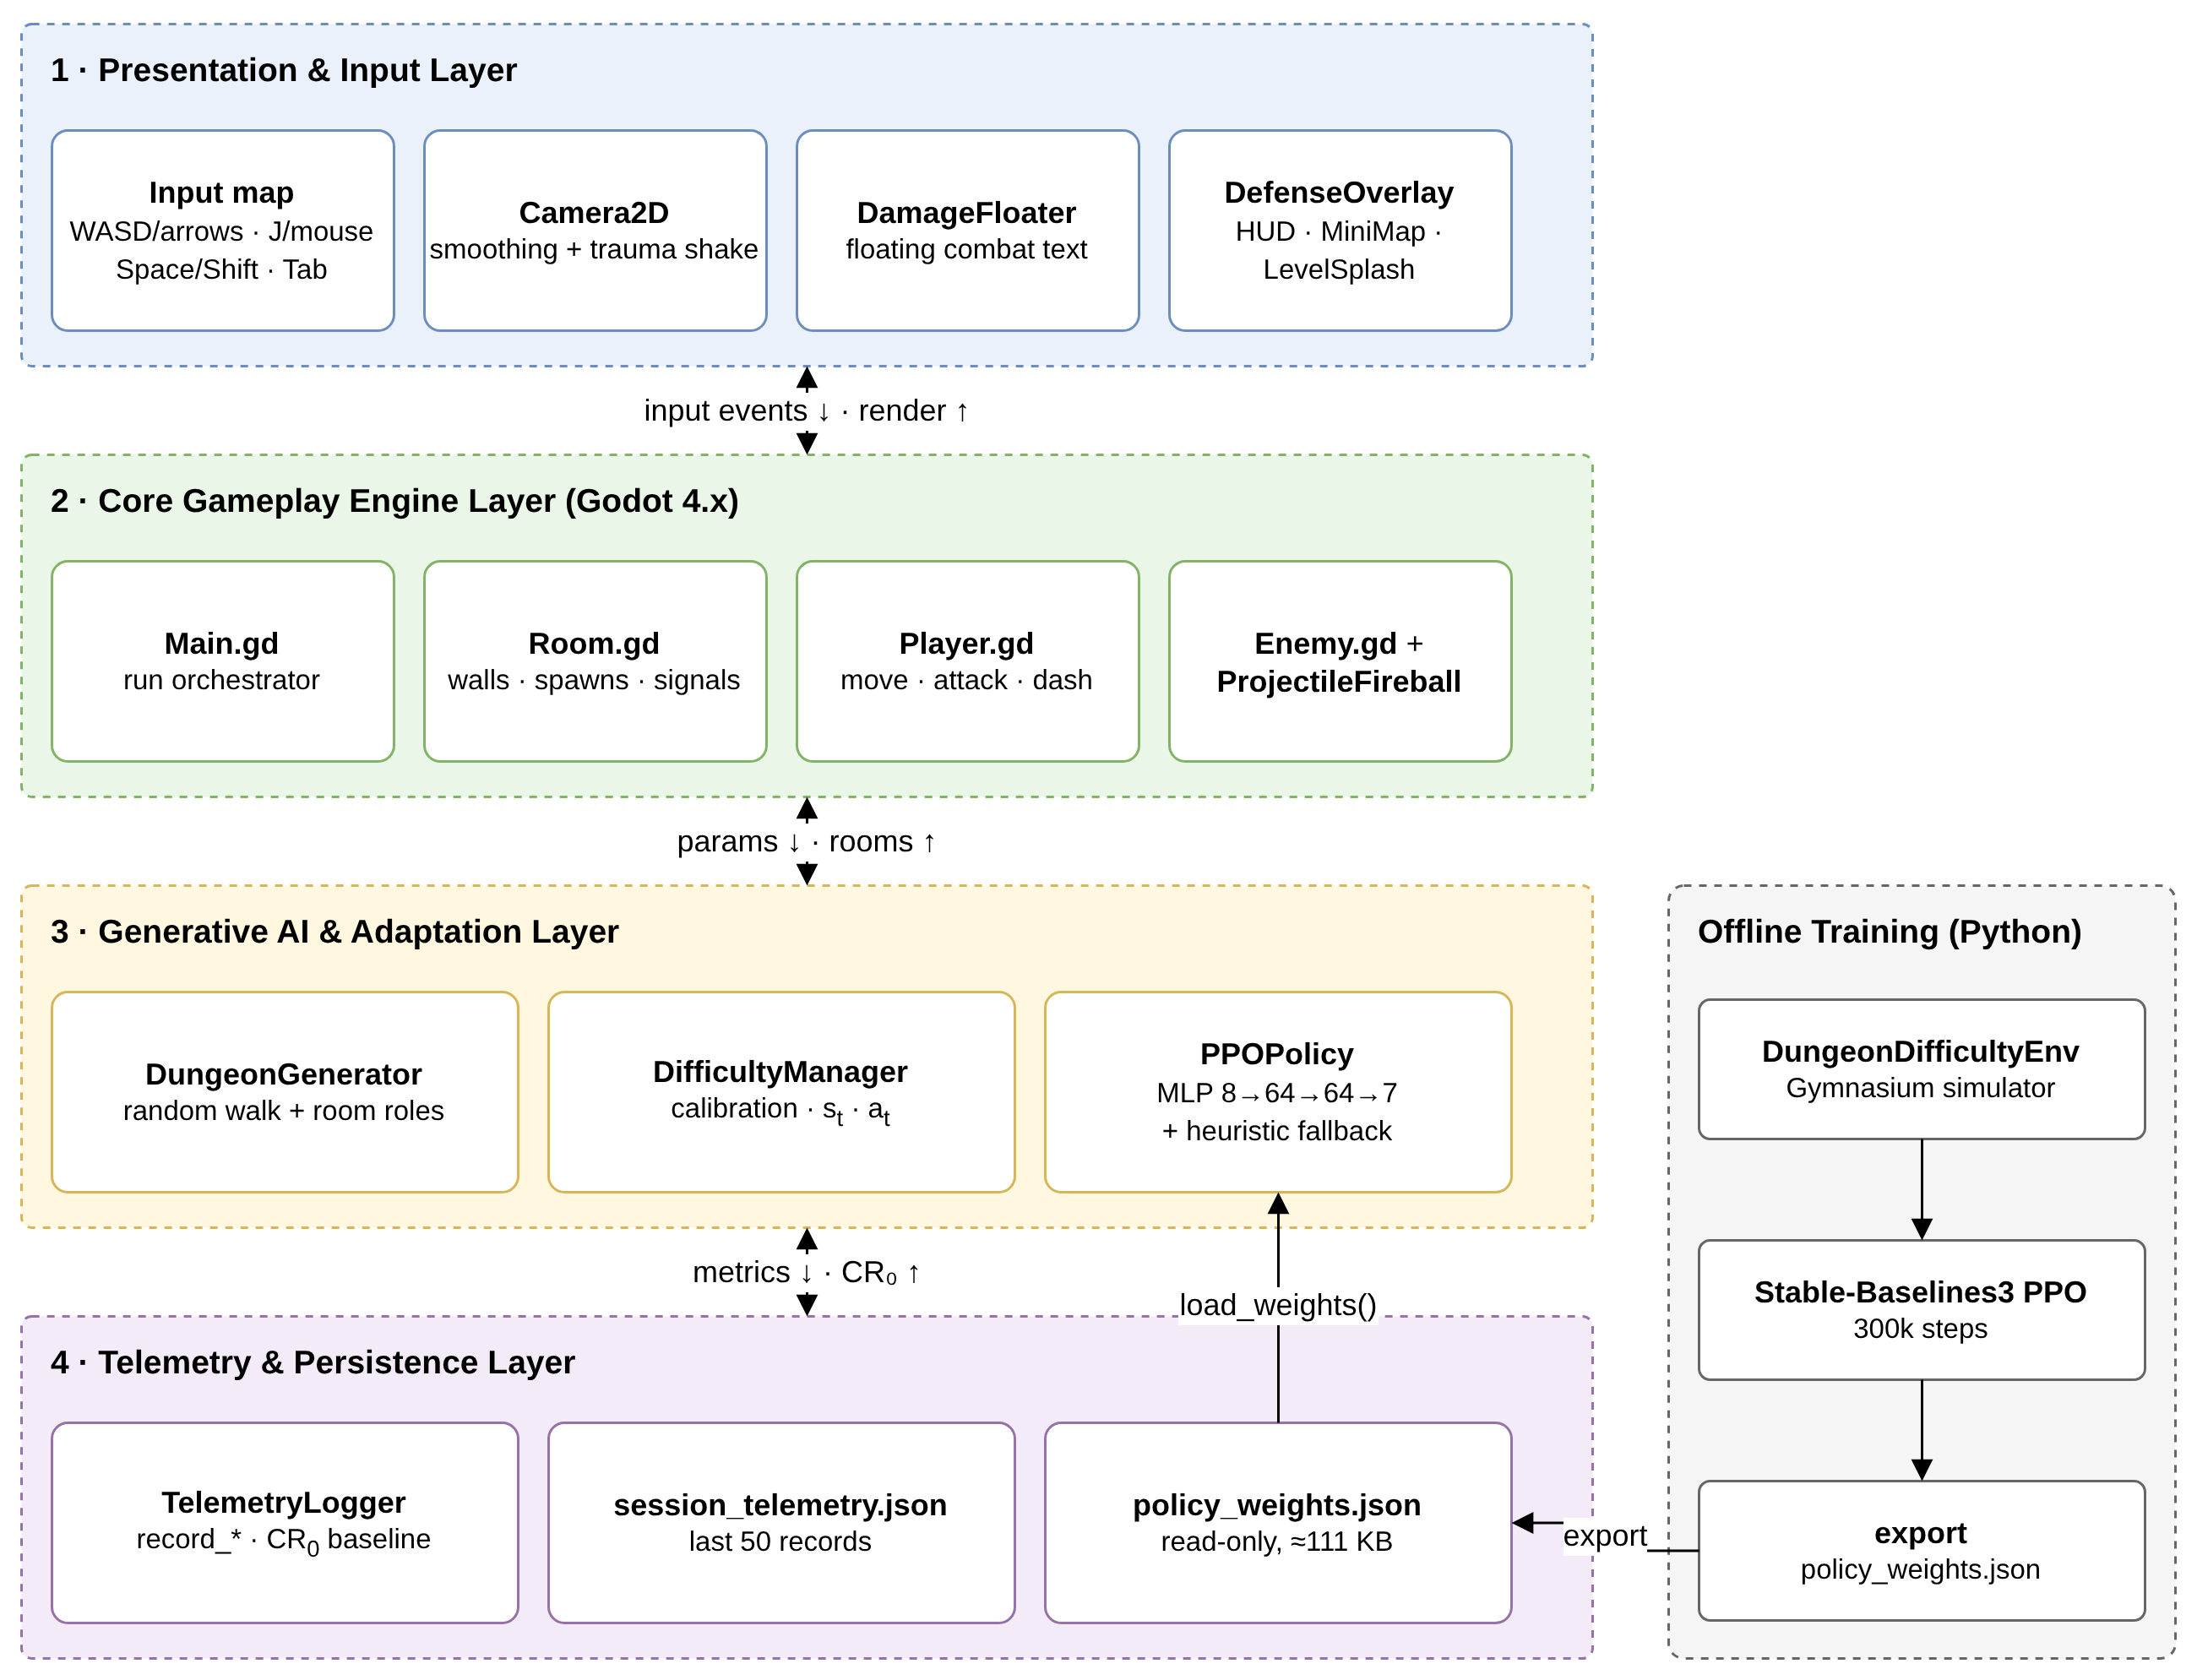
\includegraphics[width=0.95\textwidth]{ThesisFigs/fig_5_1_system_architecture.png}
\caption{Four-Tier System Architecture of Project FORGE}
\label{fig:sys_arch}
\end{figure}

\section{Architectural Components}
The primary responsibilities of the core engine components are detailed below:
\begin{itemize}
    \item \textbf{\texttt{Main.gd}:} The central gameplay orchestrator. Coordinates room transitions, scene loading, camera attachment, player death and respawn cycles, trauma camera shake dampening, and inter-floor progression.
    \item \textbf{\texttt{DifficultyManager.gd}:} Acts as the bridge between raw game parameters and the AI policy. Manages the 5-floor cold-start calibration, scales parameters deterministically under Static Baseline mode, normalizes telemetry observations ($s_t$), and denormalizes PPO actions ($a_t$) into concrete bounds.
    \item \textbf{\texttt{DungeonGenerator.gd}:} Executes Stage 1 generation. Generates a grid of rooms by random walk with branching, opens matching doors between neighbouring rooms, designates the Manhattan-farthest room as the Exit, and assigns the remaining rooms Hazard, Treasure or Combat roles. Because every room is attached to an already placed room, the layout is a connected tree by construction.
    \item \textbf{\texttt{PPOPolicy.gd}:} Contains the neural network forward pass. Loads exported JSON weights, executes the matrix multiplications with $\tanh$ hidden activations in native GDScript, clips the linear output layer to $[-1,1]$ exactly as Stable-Baselines3 does for a deterministic action, and triggers a deterministic heuristic fallback if weights are missing or unparsable.
    \item \textbf{\texttt{TelemetryLogger.gd}:} Operates as an event-driven telemetry sink fed by \texttt{Main.gd}. Accumulates damage dealt, damage taken, deaths, kills, pickups and hazard hits, and at the end of Floor 5 computes $CR_0$ and the training-scale calibration averages that seed $s_0$.
    \item \textbf{\texttt{Enemy.gd} \& \texttt{ProjectileFireball.gd}:} Implements adversary behaviors. Differentiates between Melee Crawlers (chase and bite) and Ranged Pyromancers (kiting and casting telegraphed fireballs).
\end{itemize}

Figure~\ref{fig:low_level_arch} illustrates the low-level component interaction and runtime dataflow architecture, capturing the boundary between offline policy synthesis, automated continuous integration verification, and the real-time Godot 4.x subsystems.

\begin{figure}[!htbp]
\centering
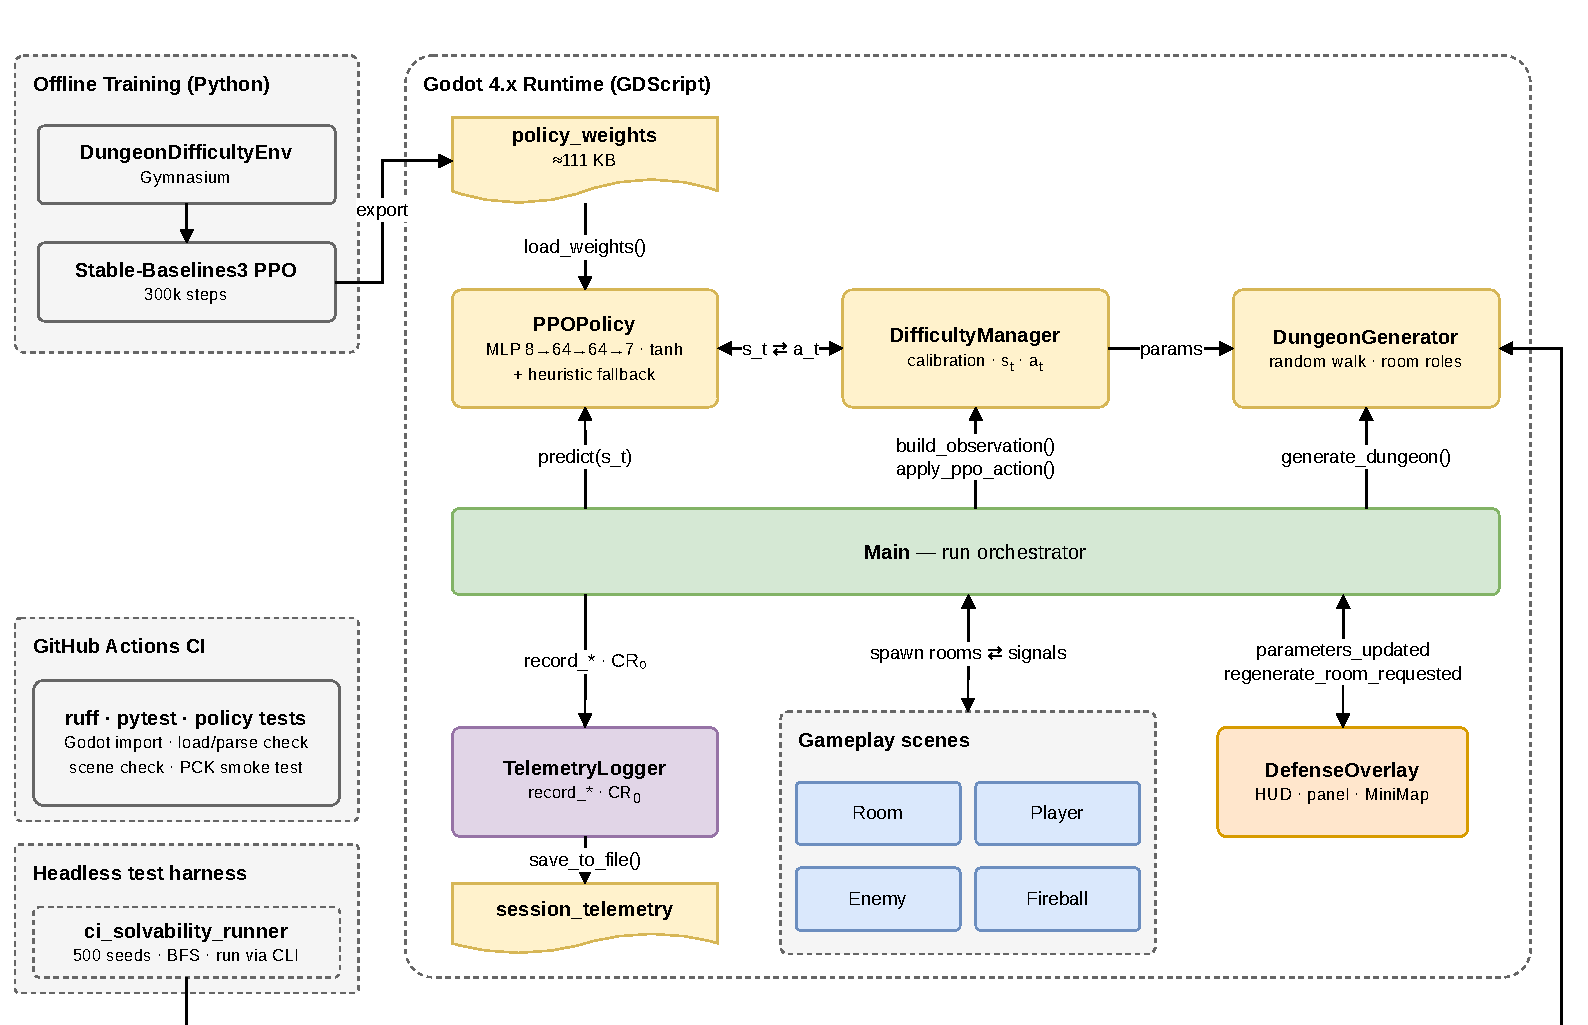
\includegraphics[width=0.95\textwidth]{ThesisFigs/fig_low_level_architecture}
\caption{Low-Level Component Interaction and Runtime Dataflow Architecture}
\label{fig:low_level_arch}
\end{figure}

\section{Interfaces and Data Contracts}

\subsection{Observation Vector Contract ($s_t \in \mathbb{R}^8$)}\label{sec:obs_contract}
At the conclusion of each floor, \texttt{DifficultyManager.gd} packages the player's recent performance into an 8-dimensional normalized observation vector $s_t$:
\begin{equation}
s_t = [s_{\text{time}}, \, s_{\text{deaths}}, \, s_{\text{dmg\_ratio}}, \, s_{\text{hp}}, \, s_{\text{dmg}}, \, s_{\text{haz}}, \, s_{\text{rooms}}, \, s_{\text{level}}]
\label{eq:obs_vector}
\end{equation}
where:
\begin{itemize}
    \item $s_{\text{time}} = \text{clamp}(t_{\text{clear}} / 90.0, 0, 1)$: Normalized floor clearing time, where $t_{\text{clear}}$ is the wall-clock time from floor start to exit ($45$\,s, i.e.\ $7.5$\,s per room on a 6-room floor, maps to $0.5$).
    \item $s_{\text{deaths}} = \text{clamp}(n_{\text{deaths}} / 3.0, 0, 1)$: Player attrition signal.
    \item $s_{\text{dmg\_ratio}} = \text{clamp}(\text{dmg\_taken} / \text{max\_hp}, 0, 1)$: Fraction of the player's maximum health lost on the floor ($0.0 = \text{untouched}, 1.0 = \text{a full health bar lost}$).
    \item $s_{\text{hp}}, s_{\text{dmg}}, s_{\text{haz}}, s_{\text{rooms}}$: Min--max normalized current values of the enemy health, enemy damage, hazard density and room count parameters (range $[0,1]$, Table~\ref{tab:param_ranges}).
    \item $s_{\text{level}} = \text{clamp}(l_{\text{current}} / 10.0, 0, 1)$: Run progression depth.
\end{itemize}
For the first adaptive floor, $s_0$ uses the same scales, but the three player signals are weighted averages over the five calibration floors (Equation~\ref{eq:s0_seed}); calibration floors with 3--5 rooms are rescaled to the 6-room convention used in training.

\subsection{Action Vector Contract ($a_t \in [-1, 1]^7$)}
The PPO actor policy predicts a 7-dimensional continuous action vector $a_t \in [-1, 1]^7$. \texttt{DifficultyManager.gd} denormalizes each component into concrete engine parameters using Table~\ref{tab:param_ranges}:
\begin{equation}
P_k = \text{low}_k + \left( \frac{a_k + 1.0}{2.0} \right) \cdot (\text{high}_k - \text{low}_k)
\label{eq:denorm}
\end{equation}

\begin{table}[!htbp]
\centering
\caption{Difficulty Parameter Mapping and Denormalization Ranges}
\label{tab:param_ranges}
\small
\begin{tabular}{p{0.06\textwidth}p{0.25\textwidth}p{0.18\textwidth}p{0.18\textwidth}p{0.22\textwidth}}
\toprule
\textbf{Index} & \textbf{Parameter Name ($P_k$)} & \textbf{Lower Bound} & \textbf{Upper Bound} & \textbf{Engine Impact} \\
\midrule
$a_0$ & Enemy Health & $20.0$\,HP & $120.0$\,HP & Base hit-points of spawned enemies \\
$a_1$ & Enemy Damage & $5.0$\,dmg & $50.0$\,dmg & Attack damage per hit / fireball \\
$a_2$ & Enemy Speed & $60.0$\,px/s & $220.0$\,px/s & Chase / kiting movement velocity \\
$a_3$ & Enemy Aggro Radius & $100.0$\,px & $450.0$\,px & Player detection distance (Pyromancers use at least $420$\,px) \\
$a_4$ & Hazard Density & $0.05$ ($5\%$) & $0.80$ ($80\%$) & Frequency of floor spike traps \\
$a_5$ & Resource Scarcity & $0.10$ ($10\%$) & $0.90$ ($90\%$) & Probability that a combat room has \emph{no} potion; fewer treasure rooms \\
$a_6$ & Room Count & $5.0$ rooms & $9.0$ rooms & Total rooms in dungeon floor \\
\bottomrule
\end{tabular}
\end{table}

Two further difficulty settings are \emph{not} part of the action vector. \texttt{enemy\_count\_scale} multiplies per-room enemy counts on the calibration floors (up to $1.3$ on Floor 5) and is reset to $1.0$ whenever a PPO action is applied, matching the training simulator. \texttt{ranged\_enemy\_ratio} (share of Pyromancers) is set on PPO floors from the linear difficulty proxy as $0.15 + 0.45\cdot\text{score}/100$; the training simulator does not model it, which is a known sim-to-real gap (Section~\ref{sec:limitations}).

\subsection{PPO Training Reward Function Formulation ($R_t$)}
During offline reinforcement learning in the Gymnasium environment (\texttt{Dungeon\-Difficulty\-Env}), the PPO policy is trained to continuously steer difficulty parameters toward the player's optimal flow channel. To eliminate reward-hacking vulnerabilities (where the agent could meet a total-time target by pinning the room count at an extreme), the reward evaluates pace on a \textit{per-room} basis and explicitly penalizes room-complexity mismatch:
\begin{equation}
R_t = (1.0 - \Delta_{\text{time}}) - 0.5 \cdot n_{\text{deaths}} - \text{pen}_{\text{pacing}} - 0.5 \cdot \Delta_{\text{rooms}}
\label{eq:reward_function}
\end{equation}
where:
\begin{itemize}
    \item $\Delta_{\text{time}} = \frac{|\bar{t}_{\text{room}} - t^*_{\text{room}}|}{t^*_{\text{room}}}$ penalizes deviation from the target clearing pace ($t^*_{\text{room}} = 7.5$\,s per room, corresponding to an optimal $45$\,s baseline clearance for a 6-room floor, with $\bar{t}_{\text{room}} = t_{\text{clear}} / n_{\text{rooms}}$).
    \item $n_{\text{deaths}}$ applies a direct attrition penalty ($0.5$ per death incurred on the floor).
    \item $\text{pen}_{\text{pacing}}$ suppresses extreme difficulty oscillations:
    \begin{equation}
    \text{pen}_{\text{pacing}} = \begin{cases}
    0.3 & \text{if } n_{\text{deaths}} = 0 \text{ and } \bar{t}_{\text{room}} < 0.5 \cdot t^*_{\text{room}} \\
    0.4 & \text{if } n_{\text{deaths}} \ge 2 \\
    0.0 & \text{otherwise}
    \end{cases}
    \end{equation}
    The first case penalizes an under-challenging floor (the policy must escalate); the second penalizes an over-punishing floor (the policy must de-escalate).
    \item $\Delta_{\text{rooms}} = \frac{|n_{\text{rooms}} - n^*_{\text{rooms}}|}{4.0}$ penalizes discrepancy between active floor room count and current combat challenge, where $n^*_{\text{rooms}} = 5.0 + 4.0 \cdot (0.5 \cdot \text{dmg}_{\text{norm}} + 0.5 \cdot \text{hp}_{\text{norm}})$, preventing the policy from trivially saturating room count at boundaries.
\end{itemize}

\section{Architecture Decisions and Technical Rationale}

\subsection{Decision 1: Pure-GDScript Forward Pass vs. External Python/ONNX Runtimes}
A pivotal architectural choice was whether to run policy inference via an external Python socket, an embedded ONNX runtime C++ GDExtension, or a native GDScript implementation.
\begin{itemize}
    \item \textbf{Trade-off Analysis:} External Python requires end-users to install Python, PyTorch, and dependencies, introducing severe deployment friction. ONNX runtimes require compiling platform-specific C++ binaries for Windows, Linux, and WebAssembly, creating portability risks.
    \item \textbf{Decision:} We implemented the matrix multiplications of the MLP ($\text{Input: 8} \rightarrow \text{Hidden: 64} \rightarrow \text{Hidden: 64} \rightarrow \text{Output: 7}$) directly in pure GDScript within \texttt{PPOPolicy.gd}.
    \item \textbf{Rationale:} Because inference occurs only once per floor transition, the computational cost is negligible (median $0.21$--$0.36$\,ms measured), and the game needs no external DLLs, so it runs on every platform Godot exports GDScript to.
\end{itemize}

\subsection{Decision 2: Two-Stage Decoupled Generation vs. End-to-End PCGRL}
In standard \texttt{gym-pcgrl}, an RL brush places walls and enemies simultaneously, frequently producing disconnected or impassable levels.
\begin{itemize}
    \item \textbf{Decision:} FORGE strictly decouples spatial layout generation (Stage 1) from combat encounter difficulty adaptation (Stage 2).
    \item \textbf{Rationale:} Decoupling makes connectivity a property of the construction: Stage 1 produces a spanning tree of rooms (checked by a breadth-first search regression test in CI) before Stage 2 populates enemies, so a player's failure is never caused by a disconnected layout. This covers room-to-room connectivity only; traversability inside rooms (e.g., hazard placement) is not formally checked.
\end{itemize}

\subsection{Decision 3: Trauma-Based Non-Linear Camera Shake}
Rather than applying linear displacement that causes visual fatigue, we implemented a trauma-based camera shake model in \texttt{Main.gd}:
\begin{equation}
\text{Offset}_x = \text{max\_offset} \cdot T^2 \cdot \text{randf\_range}(-1.0, 1.0)
\label{eq:trauma}
\end{equation}
where trauma $T \in [0, 1]$ decays linearly at $3.6$ trauma units per second (a typical hit adds $0.42$ and settles in about $0.12$\,s). Squaring trauma ($T^2$) creates impactful, satisfying visual recoil on heavy hits while preserving legibility during rapid minor combat exchanges.

\section{Design Evolution: Proposal vs. Mid-1 Architecture}
Table~\ref{tab:design_evolution} contrasts the initial Proposal-stage proof of concept with the robust architecture established for Mid-1.

\begin{table}[!htbp]
\centering
\caption{System Design Evolution: Proposal Stage vs. Mid-1 Baseline}
\label{tab:design_evolution}
\small
\begin{tabular}{p{0.22\textwidth}p{0.35\textwidth}p{0.35\textwidth}}
\toprule
\textbf{Architectural Area} & \textbf{Gate 1 Proposal State} & \textbf{Gate 3 Mid-1 Evolution} \\
\midrule
Visual Rendering & Primitive vector circles (white/red shapes) & 2D pixel-art sprites, stone tilemaps, camera trauma shake, floating combat text \\
Adversary AI & Single Melee enemy (direct pursuit only) & Multi-archetype: Melee Crawler + Ranged Pyromancer with telegraphed projectiles \\
Player Mechanics & 2D movement and static sword slash & Dynamic sword swing + Spacebar dodge roll with invulnerability frames \\
Difficulty Initialization & Hardcoded initial guess ($s_0 = \vec{0.5}$) & 5-Floor Cold-Start Protocol with weighted $CR_0$ baseline aggregation \\
Comparative Baseline & No non-adaptive baseline available & In-engine Static Baseline toggle (+8\% fixed progression) in Defense Overlay \\
CI / CD Pipeline & Manual local execution only & Automated GitHub Actions headless Godot pipeline: load check, reachability regression test, GDScript tests \\
\bottomrule
\end{tabular}
\end{table}

\section{Domain Model}\label{sec:domain}
Figure~\ref{fig:class_diagram} presents the UML class diagram illustrating the key classes, attributes, methods, and relationships.

\begin{figure}[!htbp]
\centering
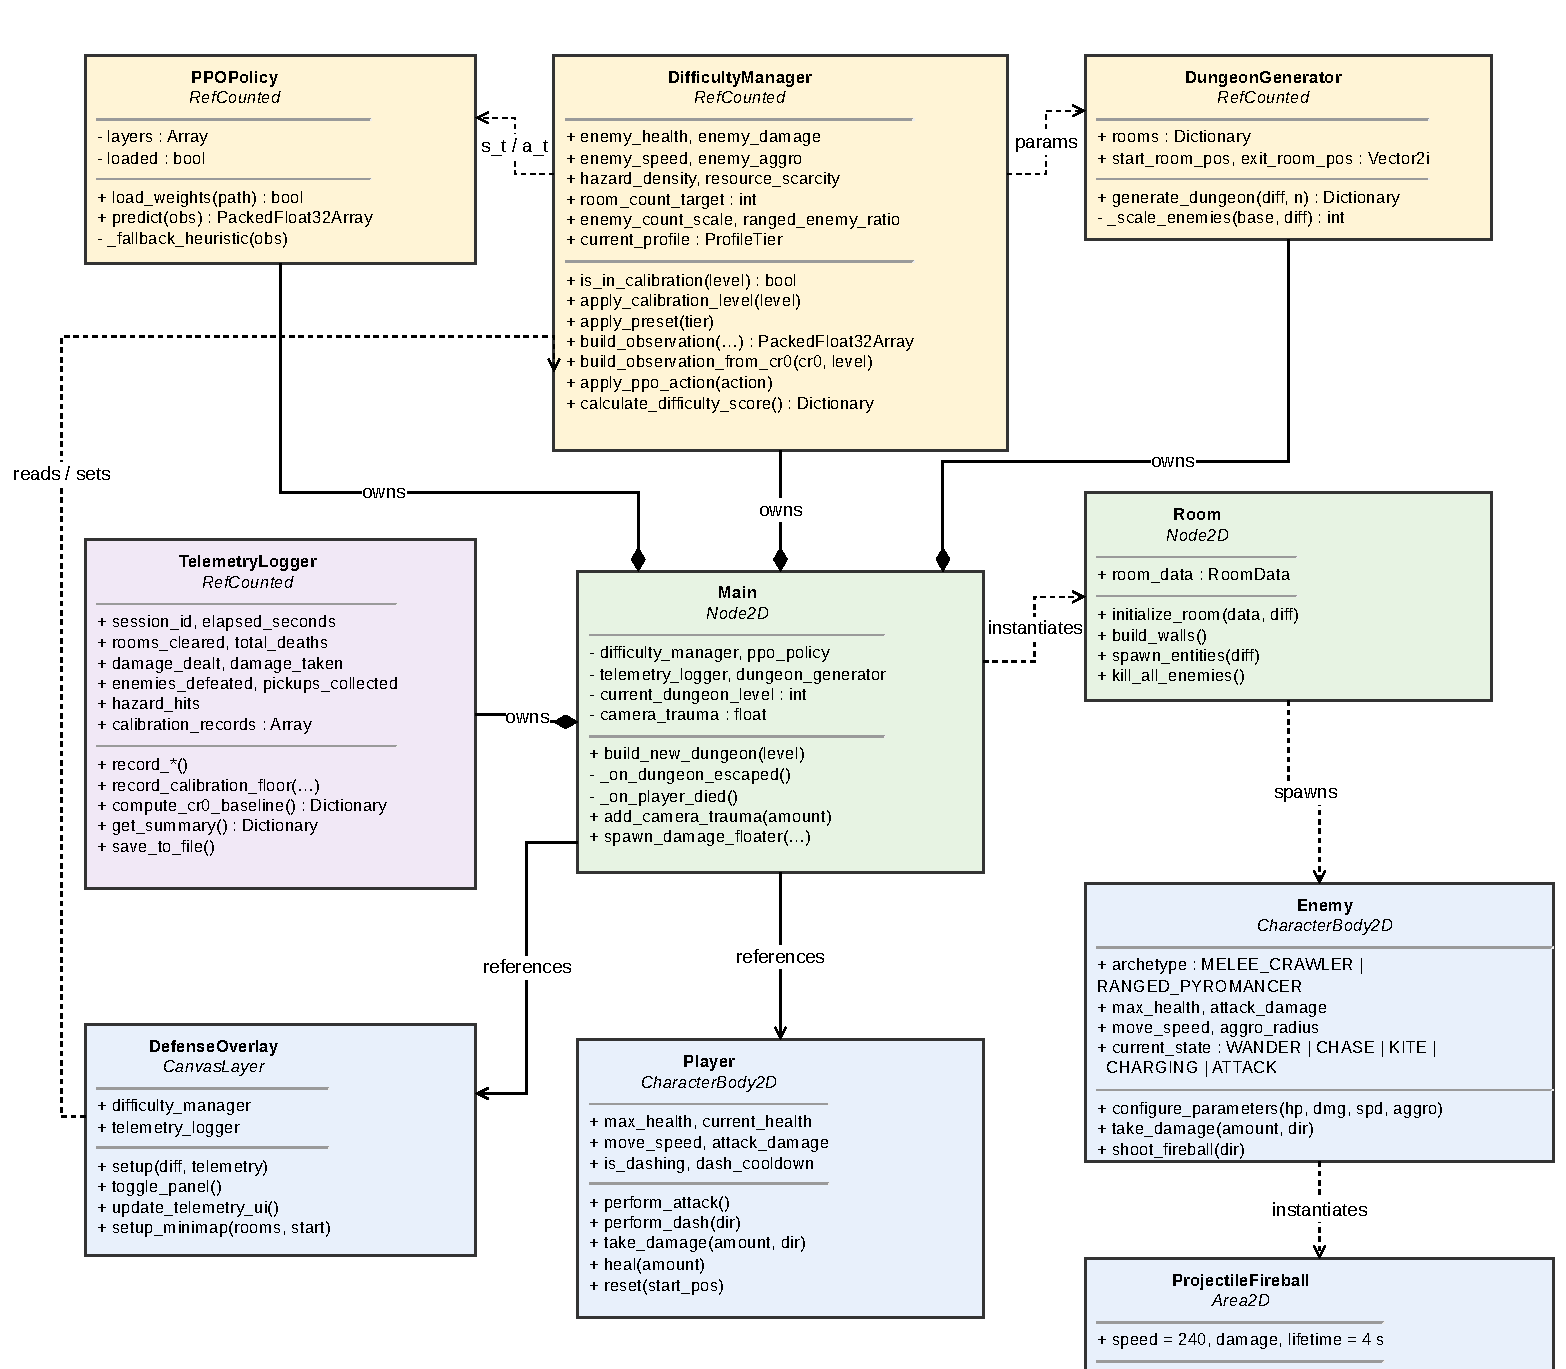
\includegraphics[width=0.98\textwidth]{ThesisFigs/fig_class_diagram}
\caption{UML Class Diagram of the Core Architecture (derived from the GDScript sources)}
\label{fig:class_diagram}
\end{figure}

\section{Data Design and Telemetry Schema}
\texttt{TelemetryLogger.gd} accumulates session metrics in memory and appends a snapshot (\texttt{get\_summary()}) to \texttt{user://session\_telemetry.json} after every room clear, every player death and every floor exit; the file keeps the most recent 50 snapshots. Table~\ref{tab:json_schema} lists the fields of one snapshot. The per-floor calibration records (floor, time, deaths, damage, rooms, difficulty score, seconds per room) are kept in memory and are used at the end of floor 5 to compute $CR_0$ and the seed observation $s_0$. Damage taken and dealt reach the logger through \texttt{Main.gd}'s \texttt{\_on\_player\_damaged} and \texttt{\_on\_enemy\_damaged} handlers (DEF-05).

\begin{table}[!htbp]
\centering
\caption[JSON Data Schema of a Telemetry Snapshot]{JSON Data Schema of a Telemetry Snapshot (\texttt{TelemetryLogger.get\_summary()})}
\label{tab:json_schema}
\small
\begin{tabular}{p{0.26\textwidth}p{0.14\textwidth}p{0.50\textwidth}}
\toprule
\textbf{Field Name} & \textbf{Data Type} & \textbf{Description \& Unit} \\
\midrule
\texttt{session\_id} & String & Session identifier of the form \texttt{sess\_<unix time>} \\
\texttt{timestamp} & Integer & Session start time (Unix seconds) \\
\texttt{elapsed\_seconds} & Float & Play time accumulated in the session (seconds) \\
\texttt{rooms\_cleared} & Integer & Rooms cleared so far \\
\texttt{total\_deaths} & Integer & Player deaths in the session \\
\texttt{damage\_dealt} & Float & Cumulative damage inflicted on enemies \\
\texttt{damage\_taken} & Float & Cumulative damage sustained by the player \\
\texttt{enemies\_defeated} & Integer & Enemies killed \\
\texttt{pickups\_collected} & Integer & Potions collected \\
\texttt{hazard\_hits} & Integer & Times the player was hit by a hazard \\
\texttt{exploration\_efficiency} & Float & Rooms cleared per minute \\
\bottomrule
\end{tabular}
\end{table}

\section{Process and Behavioral Design}

\subsection{Activity Diagram: Complete Game Session Lifecycle}
Figure~\ref{fig:activity_session} details the operational lifecycle of a gameplay session from menu initialization through cold-start calibration to closed-loop adaptive generation.

\begin{figure}[!htbp]
\centering
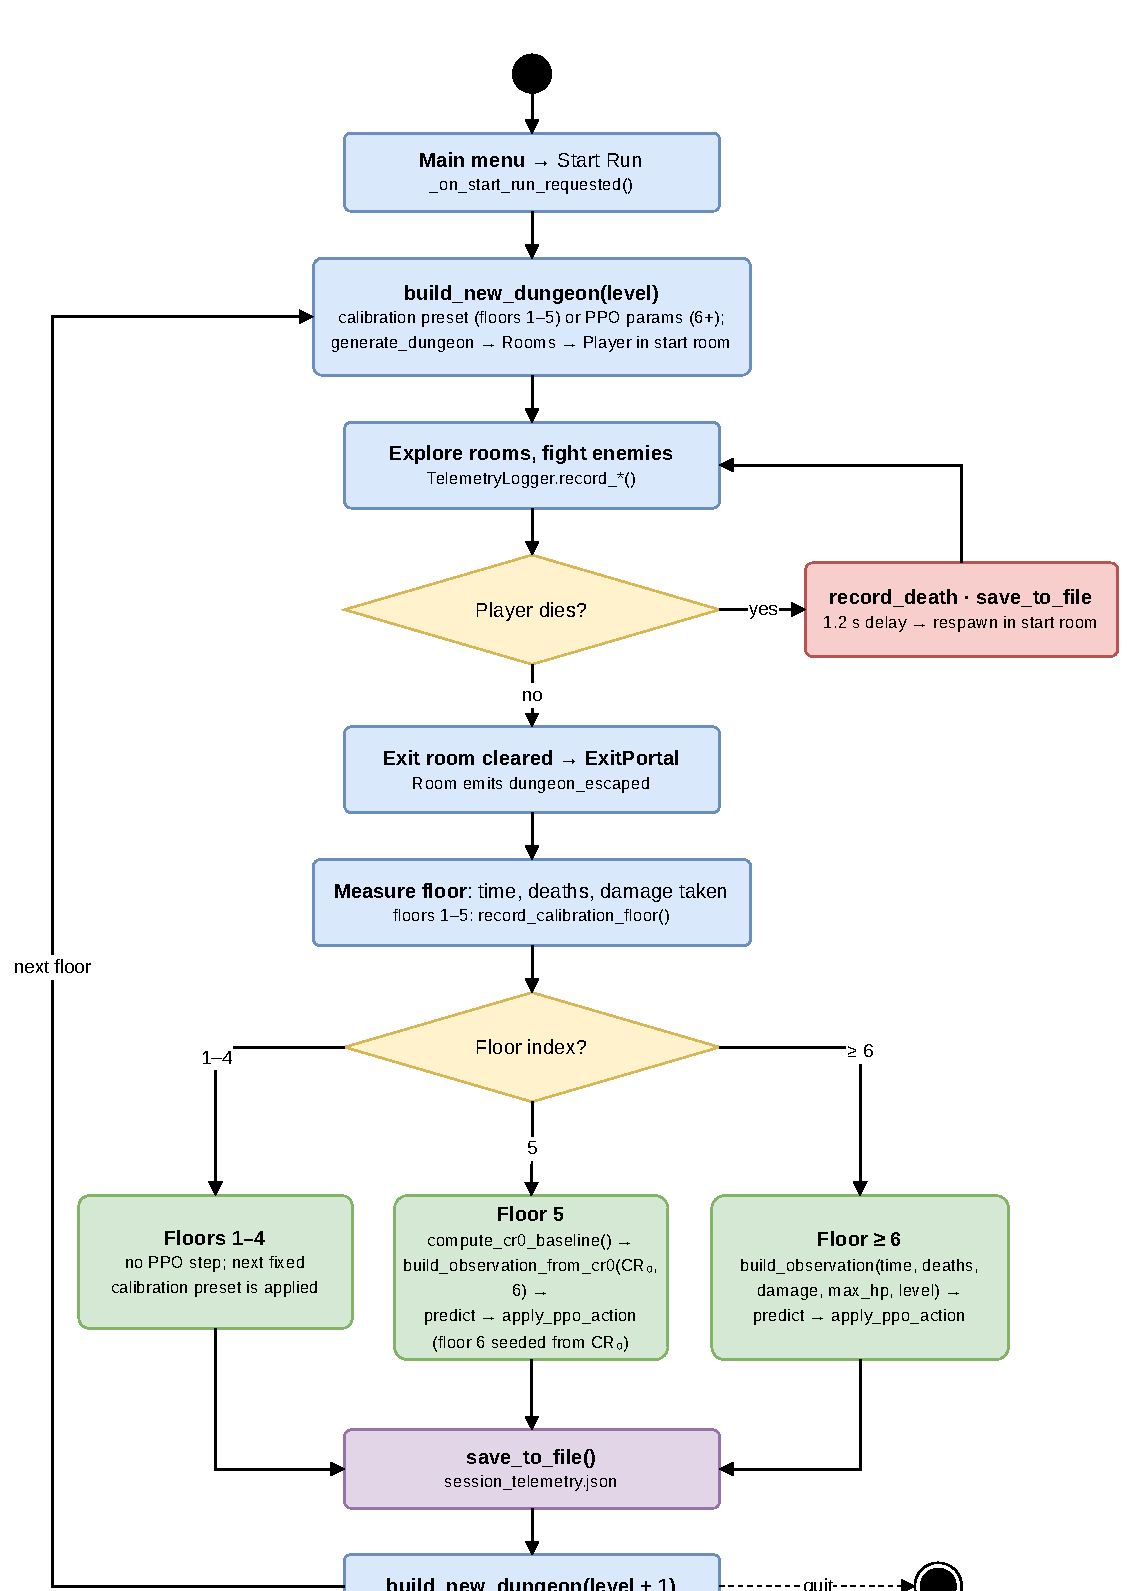
\includegraphics[width=0.65\textwidth, height=0.75\textheight, keepaspectratio]{ThesisFigs/fig_5_8_1_activity_diagram}
\caption{Activity Diagram Illustrating Complete Game Session Lifecycle}
\label{fig:activity_session}
\end{figure}

\subsection{Sequence Diagram: Inter-Floor Telemetry and Adaptation Cycle}
Figure~\ref{fig:seq_diagram} traces the message exchange when the player leaves a floor: calibration floors 1--4 only record telemetry, floor 5 computes $CR_0$ and seeds the first PPO action from the weighted calibration records ($s_0$, Equation~\ref{eq:s0_seed}), and floors 6 and above run one PPO step per floor.

\begin{figure}[!htbp]
\centering
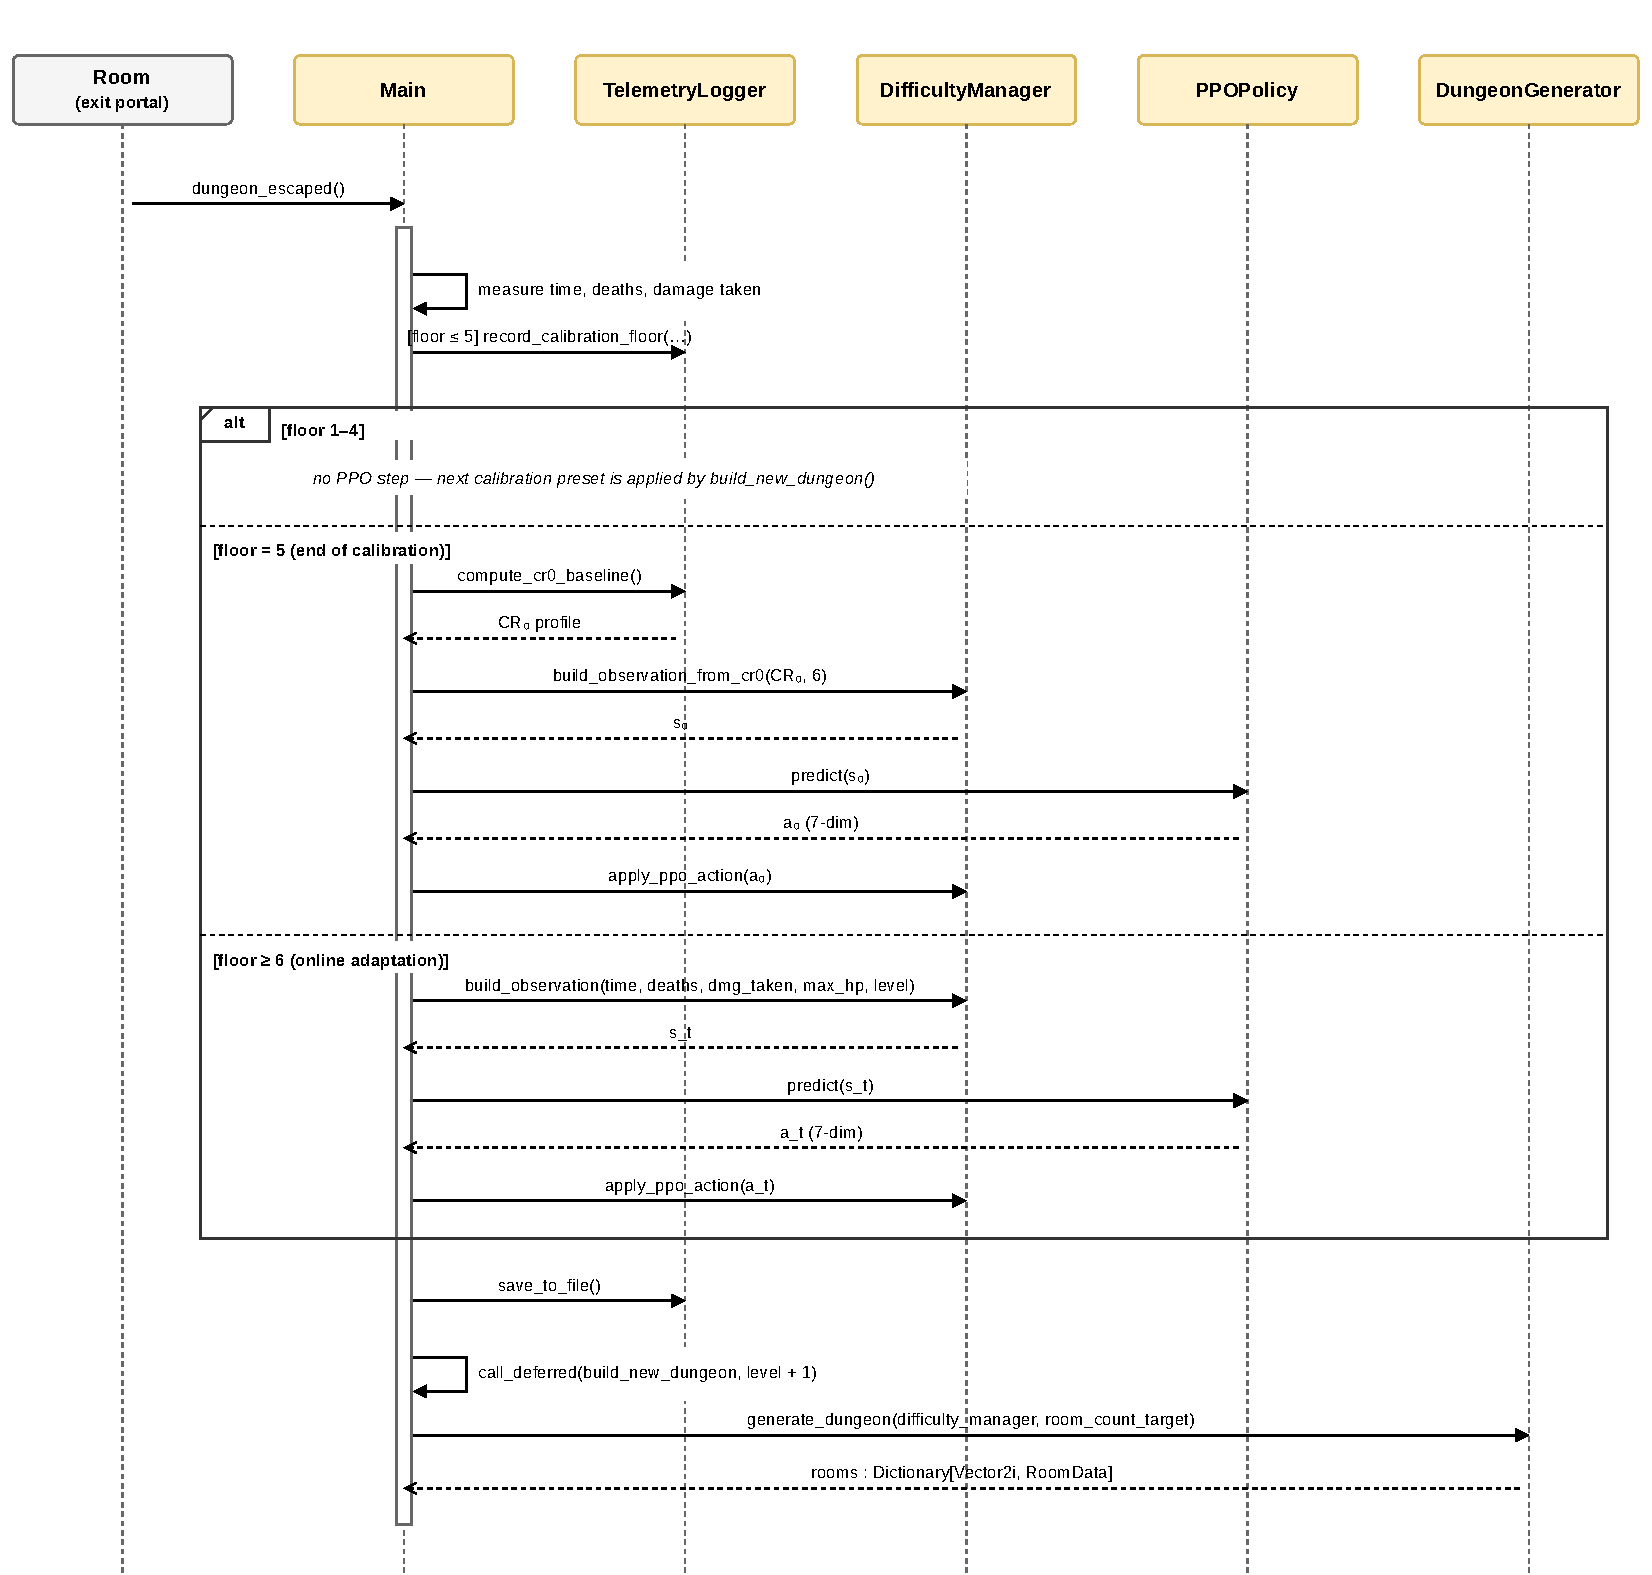
\includegraphics[width=0.98\textwidth]{ThesisFigs/fig_seq_inter_floor_adaptation}
\caption[UML Sequence Diagram of the Inter-Floor Adaptation Step]{UML Sequence Diagram of the Inter-Floor Adaptation Step (\texttt{Main.\_on\_dungeon\_escaped})}
\label{fig:seq_diagram}
\end{figure}

\subsection{State Machine Diagram: Enemy Combat AI}
Figure~\ref{fig:state_enemy} shows the finite state machines governing the two adversary archetypes in \texttt{Enemy.gd}. State changes are driven by the distance $d$ to the player rather than by timers, except for the Pyromancer's $0.5$\,s charge.

\begin{figure}[!htbp]
\centering
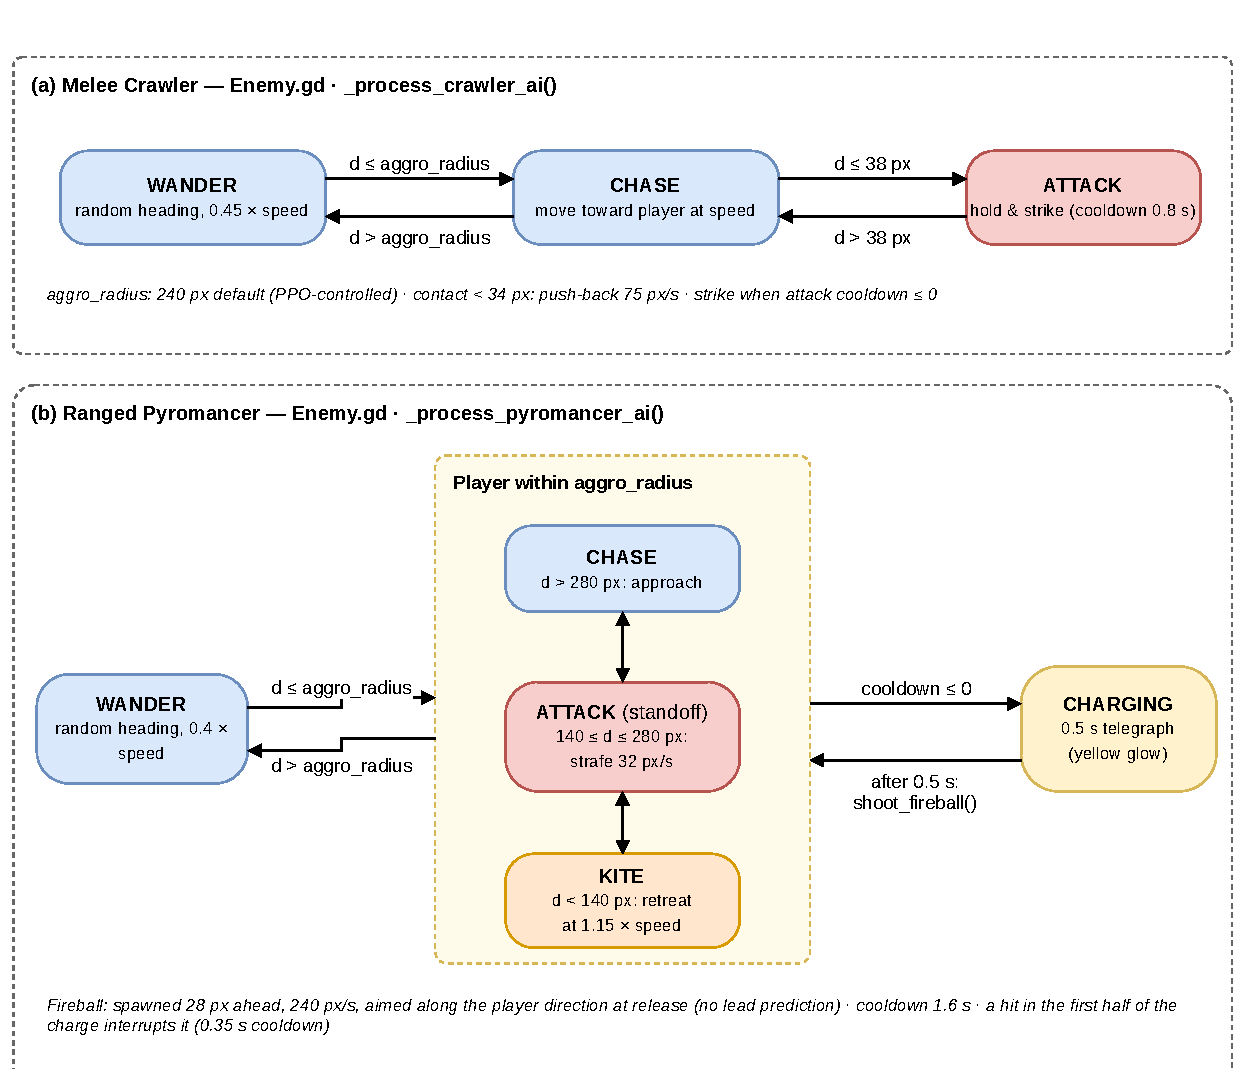
\includegraphics[width=0.85\textwidth]{ThesisFigs/fig_state_enemy_ai}
\caption[Finite State Machines of the Melee Crawler and Ranged Pyromancer]{Finite State Machines of the Melee Crawler and Ranged Pyromancer (\texttt{Enemy.gd})}
\label{fig:state_enemy}
\end{figure}

\chapter{Iteration 1: Design and Implementation}
\label{chap:iter1}

\section{Iteration Objectives}
The primary objective of Iterations 1 and 2 (Weeks 1 through 10) was transitioning Project FORGE from an exploratory proof-of-concept into a robust, literature-grounded, and visually polished mid-term deliverable. In direct alignment with the FYP Committee's directives and the FAST School of Computing CI/CD mandate, our goals were:
\begin{enumerate}
    \item \textbf{Commercial Aesthetic Elevation:} Replace all placeholder geometric shapes with 2D pixel-art sprites, integrate trauma-decay camera shake, and deploy color-coded floating combat text.
    \item \textbf{Combat Dynamics Variety:} Implement distinct adversary behavioral archetypes (Melee Crawler and Ranged Pyromancer with telegraphed projectiles) counterbalanced by a player dodge roll with invulnerability frames.
    \item \textbf{Cold-Start Calibration Protocol:} Implement an empirical 5-floor calibration sequence calculating an Initial Combat Rating ($CR_0$) to seed the PPO policy and prevent early difficulty thrashing.
    \item \textbf{Non-Adaptive Comparative Baseline:} Provide an in-engine toggle for a deterministic static roguelike baseline to benchmark adaptive generation against standard game pacing.
    \item \textbf{Automated Continuous Integration Solvability Pipeline:} Deploy a GitHub Actions workflow executing headless Godot 4.3 simulations to verify $100\%$ topological solvability on every commit.
\end{enumerate}

\section{Selected Use Cases and Feature Scope}
The implementation completed during this stage satisfies the three core use cases baselined in Chapter~\ref{chap:reqs}:
\begin{itemize}
    \item \textbf{UC-01 (Play Adaptive Session with Cold-Start Calibration):} Fully implemented and verified across Floors 1 through 5, seamlessly transitioning into closed-loop PPO generation at Floor 6.
    \item \textbf{UC-02 (Combat Encounters and Tactical Evasion):} Fully realized with dynamic melee/ranged combat, projectile kinematics, collision detection, and player dodge roll mechanics.
    \item \textbf{UC-03 (Real-Time Telemetry and Defense Inspection):} Accessible live in-engine via the \texttt{Tab} hotkey, providing real-time telemetry gauges and manual difficulty overrides.
\end{itemize}

\section{Design and Scene Architecture}
The implementation is structured around Godot 4's node composition paradigm. Figure~\ref{fig:godot_scene_tree} illustrates the primary scene hierarchy within \texttt{Main.tscn}.

\begin{figure}[!htbp]
\centering
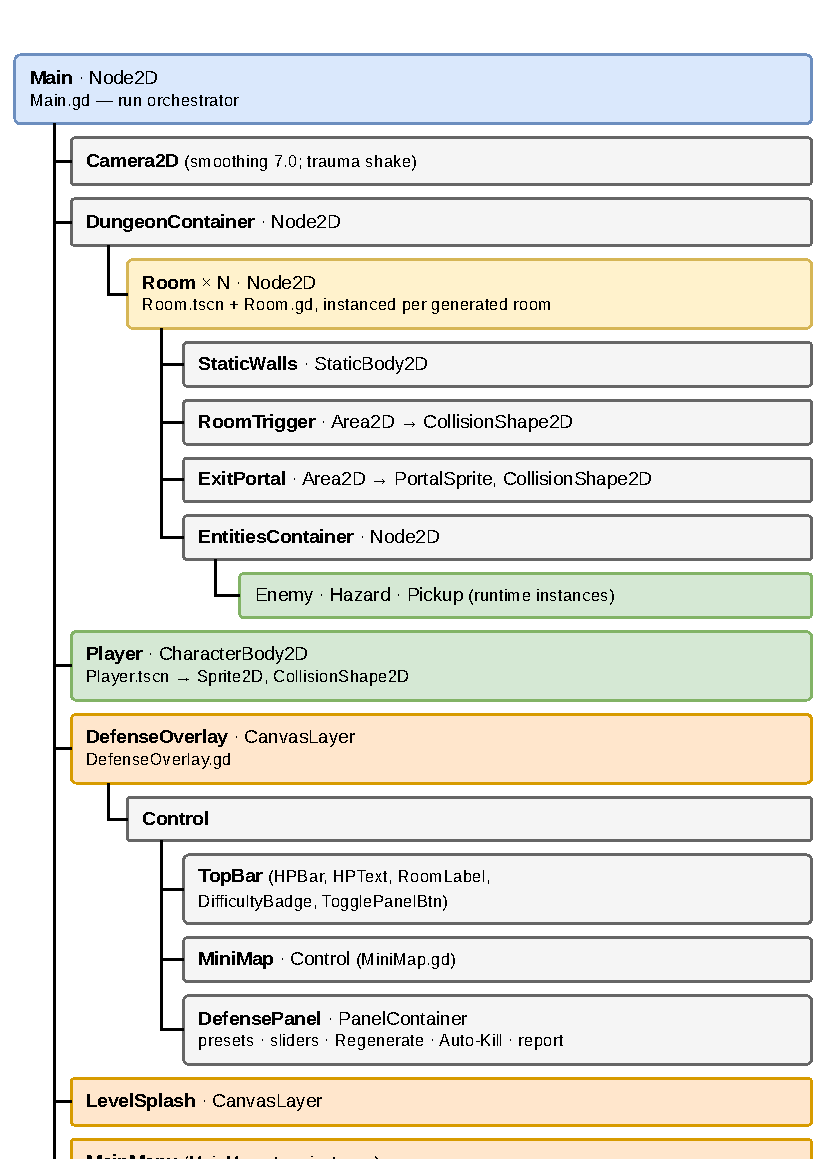
\includegraphics[width=0.65\textwidth]{ThesisFigs/fig_6_3_godot_scene_tree_hierarchy}
\caption{Godot 4.x Node Composition and Scene Tree Hierarchy}
\label{fig:godot_scene_tree}
\end{figure}

\section{Completed Features and Modules}
\label{sec:iter1_features}

\subsection{Visual Aesthetics Overhaul and Combat Juice}
Fulfilling the committee's mandate regarding visual quality:
\begin{itemize}
    \item \textbf{2D Pixel-Art Sprites:} Replaced procedural circles with top-down pixel-art assets:
    \begin{itemize}
        \item \texttt{player.png}: Armored knight with plate armor, directional facing, and dynamic sword slash animations.
        \item \texttt{enemy\_crawler.png}: Demonic melee crawler with chitinous carapace, horns, and red-eyed animation.
        \item \texttt{enemy\_pyromancer.png}: Robed occult caster with glowing staff and particle charge effects.
        \item \texttt{projectile\_fireball.png}: High-contrast fiery projectile with rotational tweening.
        \item \texttt{tile\_floor\_stone.png}: Interlocking stone flagstones with distinctive floor variants for hazard, treasure, and exit rooms.
    \end{itemize}
    \item \textbf{Camera Trauma Shake:} Integrated non-linear trauma screen shake (decay rate $3.6$\,s$^{-1}$) in \texttt{Main.gd}. Every player hit, hazard damage, or adversary elimination injects trauma ($T \leftarrow \min(T + \Delta, 1.0)$), producing visceral tactile recoil.
    \item \textbf{Floating Combat Text (\texttt{DamageFloater.tscn}):} Created an animated numerical indicator that tweens upward with scale pop upon damage events: yellow for damage inflicted on enemies, crimson red for damage taken by the player, and emerald green for health potion restoration.
    \item \textbf{Typography Polish:} Downloaded and integrated professional Google Fonts: \textbf{Cinzel} for atmospheric headers and badges, and \textbf{Inter} for HUD telemetry readouts.
\end{itemize}

\subsection{Multi-Archetype Combat Dynamics}
To eliminate combat monotony, we implemented two complementary enemy archetypes:
\begin{itemize}
    \item \textbf{Melee Crawler:} Chases the player directly upon entering aggro range ($240$\,px) at the PPO-controlled movement speed (default $125$\,px/s). Inflicts $20$ damage (default) per strike with a $0.8$\,s attack cooldown.
    \item \textbf{Ranged Pyromancer:} Maintains a tactical standoff band of $140$--$280$\,px, kiting backwards at $1.15\times$ speed when the player closes within $140$\,px. While its cooldown allows, it charges a telegraphed fireball with a $0.5$\,s yellow glow and then fires a projectile at $240$\,px/s along the direction to the player (default $18$ damage, i.e.\ $0.9\times$ the base enemy damage).
    \item \textbf{Player Dodge Roll / Dash:} Bound to the \texttt{Spacebar}, the player executes a high-speed dash ($0.2$\,s duration) granted complete invulnerability frames (iframes), governed by a $1.0$\,s cooldown bar on the HUD.
\end{itemize}

\subsection{5-Floor Cold-Start Calibration Protocol ($CR_0$ Mathematics)}
To resolve the cold-start problem inherent in RL agents, \texttt{DifficultyManager.gd} executes a structured 5-floor calibration sequence with escalating difficulty parameter tiers:
\begin{enumerate}
    \item \textbf{Floor 1 (Novice Initiation):} 3 rooms, low adversary HP ($35$), minimal damage ($10$), $5\%$ traps.
    \item \textbf{Floor 2 (Swarm Reflex):} 4 rooms, melee swarm reflexes, standard speed ($110$\,px/s), $15\%$ traps.
    \item \textbf{Floor 3 (Evasion \& Traps):} 4 rooms, high trap density ($38\%$), agile enemies ($135$\,px/s).
    \item \textbf{Floor 4 (Tactical Crucible):} 5 rooms, resilient adversaries (HP $70$, dmg $24$), $50\%$ traps.
    \item \textbf{Floor 5 (Apex Gauntlet):} 5 rooms, maximum stress test, high-speed adversaries ($175$\,px/s, dmg $30$), $65\%$ traps.
\end{enumerate}

At the exit of Floor 5, \texttt{TelemetryLogger.gd} calculates the non-uniform difficulty-weighted composite score:
\begin{equation}
\vec{w} = [1.0, \, 1.5, \, 2.0, \, 2.5, \, 3.0] \quad \left(\sum_{i=1}^5 w_i = 10.0\right)
\label{eq:weights}
\end{equation}
For each floor $i$, the engine evaluates:
\begin{align}
\text{Pace}_i &= \text{clamp}\left(1.0 - \frac{\text{sec\_per\_room}_i - 5.0}{12.0}, \, 0.0, \, 1.0\right) \\
\text{Survival}_i &= \begin{cases} 1.0 & \text{if } n_{\text{deaths}} = 0 \\ 0.5 & \text{if } n_{\text{deaths}} = 1 \\ 0.0 & \text{if } n_{\text{deaths}} \ge 2 \end{cases} \\
\text{Resistance}_i &= \text{clamp}\left(1.0 - \frac{\text{dmg\_taken}_i}{120.0}, \, 0.0, \, 1.0\right)
\end{align}
The Initial Combat Rating ($CR_0 \in [10, 95]$) is synthesized as:
\begin{equation}
CR_0 = \left(\frac{\sum w_i \cdot \text{Survival}_i}{\sum w_i} \cdot 40.0\right) + \left(\frac{\sum w_i \cdot \text{Resistance}_i}{\sum w_i} \cdot 35.0\right) + \left(\frac{\sum w_i \cdot \text{Pace}_i}{\sum w_i} \cdot 25.0\right)
\label{eq:cr0_formula}
\end{equation}
This $CR_0$ value directly seeds the initial PPO observation vector $s_0$ at Floor 6, guaranteeing that adaptive scaling begins from an accurate reflection of player skill.

\subsection{Static Non-Adaptive Roguelike Baseline Mode}
In \texttt{DefenseOverlay.gd}, the team integrated a live toggle button switching between:
\begin{itemize}
    \item \textbf{Mode: Adaptive Closed-Loop (PPO):} PPO dynamically balances encounter parameters based on live telemetry observations.
    \item \textbf{Mode: Static Baseline (Non-Adaptive):} PPO updates are bypassed; adversary health and damage scale deterministically by a flat $+8\%$ per floor, serving as the rigorous comparative control baseline required by the committee.
\end{itemize}

\section{Technical Implementation Details and Code Artifacts}

\subsection{Pure-GDScript Neural Forward Pass (\texttt{PPOPolicy.gd})}
Listing~\ref{lst:ppo_predict} presents the core matrix multiplication and activation forward pass implemented in native GDScript.

\begin{lstlisting}[language=Python, caption={Native GDScript Forward Pass Implementation in \texttt{PPOPolicy.gd}}, label={lst:ppo_predict}]
func predict(obs: PackedFloat32Array) -> PackedFloat32Array:
    if not loaded:
        return _fallback_heuristic(obs)

    var x: Array = []
    for v in obs:
        x.append(v)

    for i in range(layers.size()):
        var layer: Dictionary = layers[i]
        var w: Array = layer["w"]   # shape [out_dim][in_dim]
        var b: Array = layer["b"]   # shape [out_dim]
        var y: Array = []
        y.resize(w.size())
        for o in range(w.size()):
            var s: float = b[o]
            var row: Array = w[o]
            for k in range(row.size()):
                s += float(row[k]) * float(x[k])
            y[o] = s
        var is_last := (i == layers.size() - 1)
        if not is_last:                    # tanh on hidden layers only
            for o in range(y.size()):
                y[o] = tanh(y[o])
        x = y

    var out := PackedFloat32Array()
    for v in x:
        out.append(clampf(tanh(v), -1.0, 1.0))   # bounded output
    return out
\end{lstlisting}

\subsection{Heuristic Fallback Mechanism}
Listing~\ref{lst:fallback} shows the rule-based fallback in \texttt{PPOPolicy.gd}, used when \texttt{policy\_weights.json} is missing or cannot be parsed so that the game stays playable.

\begin{lstlisting}[language=Python, caption={Deterministic Heuristic Fallback in \texttt{PPOPolicy.gd}}, label={lst:fallback}]
func _fallback_heuristic(obs: PackedFloat32Array) -> PackedFloat32Array:
    var norm_time: float = obs[0]
    var norm_deaths: float = obs[1]
    var norm_dmg_ratio: float = obs[2]
    var cur_hp: float = obs[3]
    var cur_dmg: float = obs[4]
    var cur_haz: float = obs[5]
    var cur_rooms: float = obs[6]

    # > 0: player did well -> escalate, < 0: player struggled -> ease off
    var performance_signal: float = (0.5 - norm_time) * 1.4 \
        - norm_deaths * 1.5 - norm_dmg_ratio * 0.8
    performance_signal = clampf(performance_signal, -1.0, 1.0)

    var step := 0.12   # per-level nudge, in normalized [-1, 1] units
    var out := PackedFloat32Array()
    out.append(clampf(cur_hp * 2.0 - 1.0 + performance_signal * step, -1.0, 1.0))
    out.append(clampf(cur_dmg * 2.0 - 1.0 + performance_signal * step, -1.0, 1.0))
    out.append(clampf(performance_signal * 0.5, -1.0, 1.0))   # enemy_speed
    out.append(clampf(performance_signal * 0.5, -1.0, 1.0))   # enemy_aggro
    out.append(clampf(cur_haz * 2.0 - 1.0 + performance_signal * step, -1.0, 1.0))
    out.append(clampf(performance_signal * 0.3, -1.0, 1.0))   # resource_scarcity
    out.append(clampf(cur_rooms * 2.0 - 1.0 + performance_signal * step, -1.0, 1.0))
    return out
\end{lstlisting}

\subsection{Ranged Pyromancer Projectile Instantiation}
In \texttt{Enemy.gd}, a Ranged Pyromancer that is within aggro range and off cooldown enters the \texttt{CHARGING} state for $0.5$\,s and then calls \texttt{shoot\_fireball()}:
\begin{lstlisting}[language=Python, caption={Telegraphed Fireball Spawning in \texttt{Enemy.gd}}, label={lst:enemy_attack}]
# in _process_pyromancer_ai(): telegraph, then fire
if is_charging:
    current_state = State.CHARGING
    charge_timer += delta
    move_velocity = -dir_to_player * 18.0       # hold ground while casting
    if charge_timer >= charge_duration:         # 0.5 s telegraph
        is_charging = false
        shoot_fireball(dir_to_player)
    return move_velocity

func shoot_fireball(target_dir: Vector2) -> void:
    attack_cooldown_timer = attack_rate
    if projectile_scene:
        var p = projectile_scene.instantiate()
        var spawn_pos = global_position + target_dir * 28.0
        get_parent().add_child(p)
        p.setup(target_dir, spawn_pos, attack_damage, 240.0)
        apply_knockback(-target_dir * 90.0)
\end{lstlisting}

\section{Tools, Frameworks and Technologies Used}
Table~\ref{tab:tech_stack} summarizes the technology stack employed during Iterations 1 and 2.

\begin{table}[!htbp]
\centering
\caption{FORGE Technology Stack and Infrastructure}
\label{tab:tech_stack}
\small
\begin{tabular}{p{0.25\textwidth}p{0.25\textwidth}p{0.45\textwidth}}
\toprule
\textbf{Layer / Domain} & \textbf{Technology} & \textbf{Role in FORGE Architecture} \\
\midrule
Game Engine & Godot 4.3 (CI target); developed on 4.7.2 & Core 2D physics, tilemaps, node hierarchy, visual rendering. \\
In-Game Scripting & GDScript 2.0 & High-performance native engine logic and embedded neural forward pass. \\
Offline RL Training & Python 3.12 / SB3 & Gymnasium environment, PPO policy optimization, weight export. \\
Neural Framework & PyTorch $\ge 2.0$ & Multilayer Perceptron tensor operations and gradient calculations. \\
Continuous Integration & GitHub Actions & Automated headless Godot syntax compilation and solvability validation. \\
Version Control & Git / GitHub & Distributed source management, atomic commits, and release tagging. \\
Typography \& Assets & Google Fonts / Pixel Art & Cinzel, Inter typography; custom 2D dungeon sprite sheets. \\
\bottomrule
\end{tabular}
\end{table}

\section{Demonstration Evidence}
The implemented system was validated through live gameplay sessions and headless test suites:
\begin{itemize}
    \item \textbf{Aesthetic Verification:} Pixel-art sprites seamlessly render on dynamic stone tilemaps with $0$\,ms stutter. Trauma camera shake triggers with visible physical impact upon taking damage.
    \item \textbf{Tactical Evasion Evidence:} Spacebar dodge rolls reliably grant iframes, allowing players to roll through Pyromancer fireballs without sustaining damage.
    \item \textbf{Telemetry Verification:} Flat JSON telemetry files (\texttt{session\_telemetry.json}) correctly log room entry/exit timestamps, damage numbers, and $CR_0$ scores across sessions.
    \item \textbf{Defense Overlay Inspector:} Evaluators can press \texttt{Tab} in real-time to toggle between PPO Adaptive and Static Baseline modes, observe live parameter numbers, and adjust sliders dynamically.
\end{itemize}

\section{Iteration Outcome}
Iterations 1 and 2 successfully resolved all committee directives and mid-term commitments. The prototype functions as an authentic, visually polished 2D combat roguelike powered by a deterministic, mathematically verified two-stage procedural dungeon generator with embedded reinforcement learning difficulty conditioning.

\chapter{Testing and Early Validation}
\label{chap:testing}

\section{Testing Strategy}
To guarantee system stability, algorithmic reliability, and gameplay solvability, Project FORGE employs a structured multi-tier verification strategy. Because FORGE operates at the intersection of game engine physics, procedural generation, and machine learning, testing spans four distinct levels:
\begin{enumerate}
    \item \textbf{Unit Testing:} Validating core mathematical routines, observation vector normalization, action denormalization clamping, and non-uniform $CR_0$ weighting formulas.
    \item \textbf{Engine Integration Testing:} Verifying node lifecycles, signal dispatching between \texttt{Player.gd}, \texttt{Enemy.gd}, and \texttt{Main.gd}, combat collision layer masks, and projectile lifespan cleanup.
    \item \textbf{Automated Headless CI Solvability Testing:} Executing Godot 4.3 in \texttt{--headless} mode via GitHub Actions across 500 randomized seeds to mathematically verify $100\%$ door connectivity and breadth-first-search reachability over the door graph.
    \item \textbf{Simulated Policy Evaluation:} Evaluating the offline PPO policy in Gymnasium (training curves over three seeds and 100 paired 30-level episodes per simulated player profile, Section~\ref{sec:policy_eval}) to verify pacing and detect reward hacking.
\end{enumerate}

\section{Test Levels and Techniques}
Table~\ref{tab:test_levels} details the specific techniques, tools, and execution environments applied across each testing tier.

\begin{table}[!htbp]
\centering
\caption{FORGE Multi-Tier Verification Framework}
\label{tab:test_levels}
\small
\begin{tabular}{p{0.20\textwidth}p{0.22\textwidth}p{0.28\textwidth}p{0.22\textwidth}}
\toprule
\textbf{Test Level} & \textbf{Scope} & \textbf{Technique / Tool} & \textbf{Execution Environment} \\
\midrule
Unit Tests & Math \& data serialization & Assertion scripts (\texttt{pytest}, GDScript) & Local CLI \& Godot Editor \\
Integration Tests & Combat \& scene transitions & Live interactive test scenes & Godot 4.x Runtime \\
Automated Solvability & Layout reachability (BFS) & Headless seed harness script & GitHub Actions CI (Ubuntu) \\
Policy Validation & Stability \& reward bounds & Training curves and paired profile evaluation & Python 3.12 / Stable-Baselines3 \\
\bottomrule
\end{tabular}
\end{table}

\section{Formal Test Suite and Test Cases}
Table~\ref{tab:test_cases} documents the primary test suite (TC-01 through TC-10) executed during Iteration 2.

\begin{table}[!htbp]
\centering
\caption{Formal Test Suite and Execution Results}
\label{tab:test_cases}
\scriptsize
\begin{tabular}{p{0.06\textwidth}p{0.18\textwidth}p{0.24\textwidth}p{0.24\textwidth}p{0.14\textwidth}p{0.06\textwidth}}
\toprule
\textbf{Test ID} & \textbf{Component} & \textbf{Test Description} & \textbf{Input / Conditions} & \textbf{Expected Result} & \textbf{Status} \\
\midrule
TC-01 & \texttt{TelemetryLogger} & Telemetry event capture & Player takes damage, inflicts hits, clears room & Log dictionary records exact health deltas & Pass \\
TC-02 & \texttt{TelemetryLogger} & Cold-Start $CR_0$ calculation & Complete 5 floors with varying clearing times & $CR_0$ computes correctly in $[10, 95]$ via $\vec{w}$ & Pass \\
TC-03 & \texttt{PPOPolicy} & Neural forward pass math & Feed 8D normalized vector $s_t \in [0, 1]^8$ & Returns 7D vector $a_t \in [-1, 1]^7$ in $<1$\,ms & Pass \\
TC-04 & \texttt{PPOPolicy} & Zero-crash heuristic fallback & Delete/corrupt \texttt{policy\_weights.json} & Falls back to heuristic without game crash & Pass \\
TC-05 & \texttt{DifficultyMgr} & Action denormalization & Inject action $a = [-1.0, 1.0, \dots]$ & Parameters mapped to exact table ranges & Pass \\
TC-06 & \texttt{DungeonGen} & Headless BFS Solvability & Generate 500 dungeons with random seeds & $100\%$ seeds have valid path to exit & Pass \\
TC-07 & \texttt{Enemy} & Melee Crawler AI & Player enters $240$\,px detection radius & Enemy pursues directly; bites on contact & Pass \\
TC-08 & \texttt{Enemy} & Ranged Pyromancer AI & Player enters aggro; range $200$\,px & Shows $0.5$\,s tell; spawns fireball projectile & Pass \\
TC-09 & \texttt{Player} & Dodge roll invulnerability & Spacebar press during incoming fireball & Player dashes; receives zero damage & Pass \\
TC-10 & \texttt{DefenseOverlay} & Static baseline toggle & Toggle button in Tab overlay & Stats scale by exactly $+8\%$ per floor & Pass \\
\bottomrule
\end{tabular}
\end{table}

\section{Test Results and Analysis}
All 10 formal test cases passed successfully. Key findings include:
\begin{itemize}
    \item \textbf{Neural Forward Pass Performance:} Measured with the reproducible script \texttt{tests/benchmark\_inference.gd} (headless Godot 4.7.2, 200 warm-up and 1,000 timed calls of \texttt{PPOPolicy.predict()} on the shipped weights), the mean latency was $0.212$\,ms (median $0.210$\,ms, 95th percentile $0.223$\,ms, 99th percentile $0.241$\,ms, maximum $0.355$\,ms), with no invalid outputs. The mean uses about $1.3\%$ of the $16.6$\,ms frame budget and the maximum is roughly $2.1\%$, well inside the $<1.0$\,ms bound of NFR-06 and imperceptible at 60\,FPS.
    \item \textbf{Topological Solvability:} In automated CI runs executing \texttt{DungeonGenerator.gd} across 500 randomized seeds, 500 out of 500 layouts established a continuous, walkable path between the player spawn and the exit portal ($100\%$ pass rate).
    \item \textbf{Cold-Start Numerical Stability:} The non-uniform weighting formula (Equations~\ref{eq:weights}--\ref{eq:cr0_formula}, with the clamp to $[10, 95]$) was evaluated on three scripted profiles; the values below are computed from the stated per-floor inputs:
    \begin{itemize}
        \item Novice (pace 10, 12, 15, 15, 15\,s/room; deaths 0, 0, 2, 2, 2; damage 60, 80, 120, 120, 120): $CR_0 \approx 19.6$.
        \item Intermediate ($9$\,s/room, one death on Floors 4 and 5, $70$ damage per floor): $CR_0 \approx 60.2$.
        \item Expert ($4.5$\,s/room, no deaths, no damage): raw score $100$, clamped to $CR_0 = 95$.
    \end{itemize}
\end{itemize}


\section{Training Convergence and Unseen-Profile Evaluation}
\label{sec:policy_eval}
To address the committee's request for evidence that the learned policy is better than an untrained one, the PPO training run was repeated with logging enabled (same environment, network ($8\rightarrow64\rightarrow64\rightarrow7$), hyper-parameters and 300{,}000 timesteps as \texttt{train\_ppo\_difficulty.py}) for three random seeds. The shipped \texttt{policy\_weights.json} was evaluated separately using a NumPy re-implementation of the forward pass in \texttt{PPOPolicy.gd}.

\subsection{Training Curves}
Figure~\ref{fig:training_curves} shows the three runs. The mean episode return (30 levels per episode) rises from about $-6.5$ at initialization to $16.0$, $15.8$ and $16.2$ for seeds 0, 1 and 2 respectively, and flattens after roughly 250k timesteps. The policy's exploration standard deviation decreases monotonically from $1.0$ to about $0.6$, and the critic loss settles near a stable plateau; no run diverged.

\begin{figure}[!htbp]
\centering
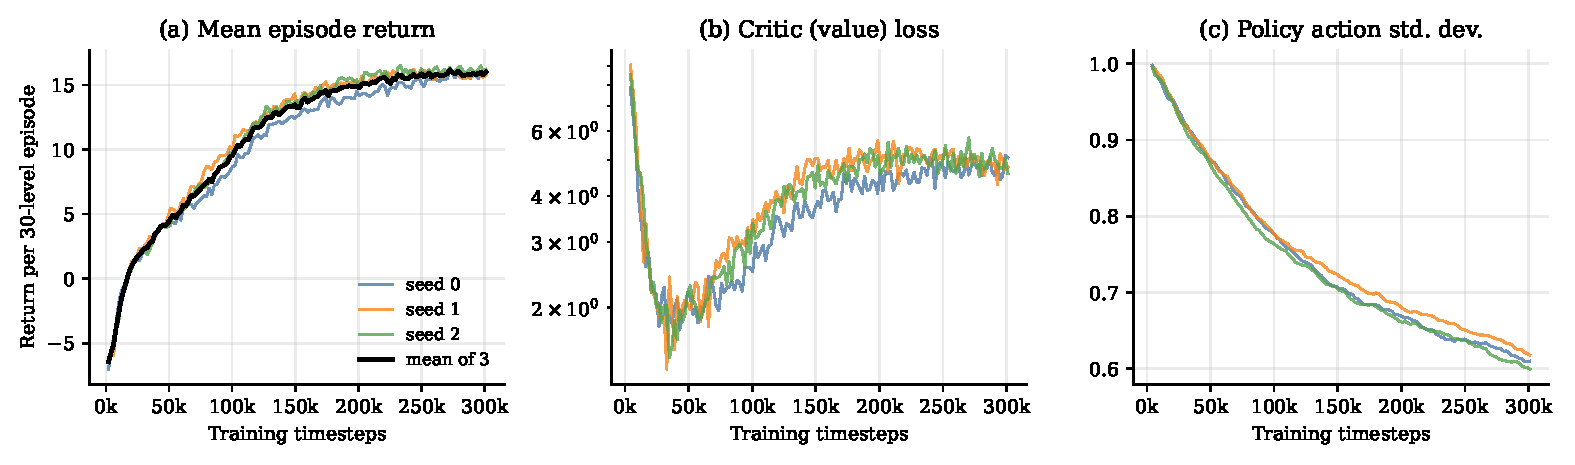
\includegraphics[width=\textwidth]{ThesisFigs/fig_training_curves}
\caption{PPO training curves for three random seeds: (a) mean episode return, (b) value-function loss, (c) action standard deviation.}
\label{fig:training_curves}
\end{figure}

\subsection{Trained vs.\ Randomly Initialized Policy on Unseen Player Profiles}
\textbf{Protocol.} The simulated player in training starts with skill $\sim U(0.3,0.6)$. Evaluation used profiles with initial skill $0.10$, $0.20$ (novice) and $0.70$, $0.80$, $0.90$ (skilled/expert), none of which occur in training, plus $0.45$ as an in-range reference. Each profile was played for 100 episodes of 30 levels using identical random seeds for every policy (paired comparison). The baseline is a randomly initialized policy: ten untrained networks with the same architecture, deterministic output, averaged. Besides the training reward, two reward-independent metrics are reported: the pacing error $|t_{\text{room}}-7.5\,\text{s}|/7.5\,\text{s}$ and deaths per level.

\begin{figure}[!htbp]
\centering
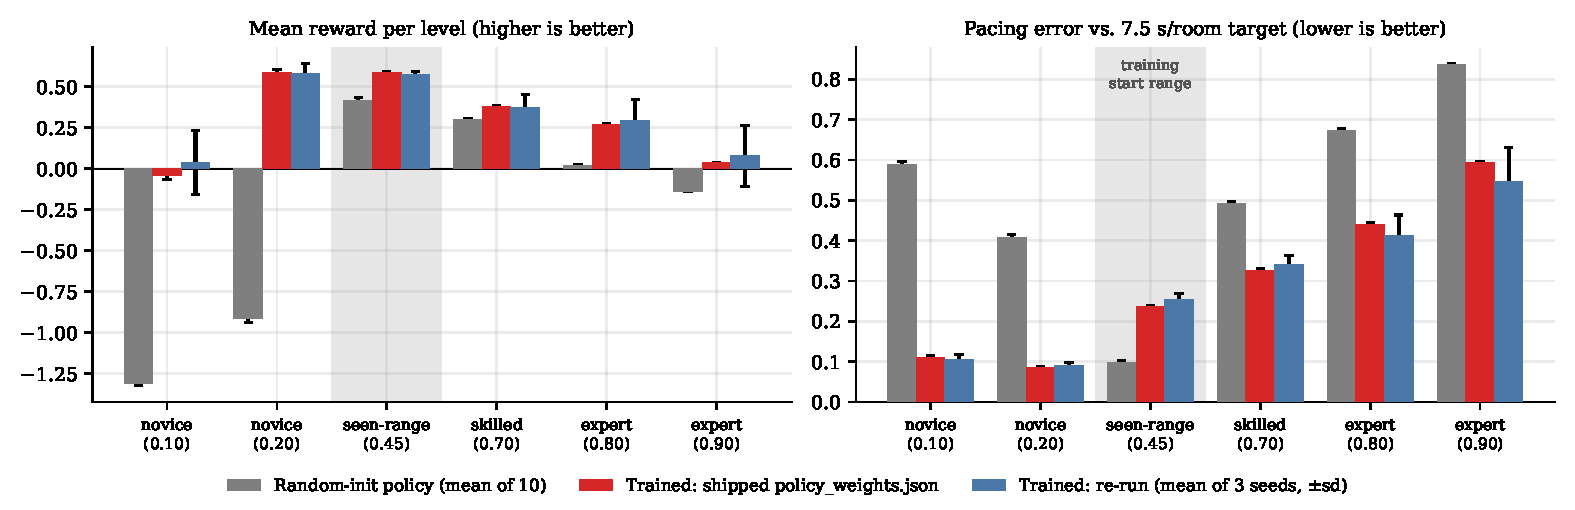
\includegraphics[width=\textwidth]{ThesisFigs/fig_policy_eval}
\caption{Mean reward per level (left) and pacing error (right) on simulated player profiles. The shaded band marks the skill range seen in training; error bars are 95\% confidence intervals (shipped, random-init) or the standard deviation over seeds (re-run).}
\label{fig:policy_eval}
\end{figure}

\begin{table}[!htbp]
\centering
\caption{Randomly initialized vs.\ trained policy on simulated player profiles (100 paired episodes per profile).}
\label{tab:policy_eval}
\scriptsize
\begin{tabular}{p{0.22\textwidth}cccccccc}
\toprule
& \multicolumn{3}{c}{\textbf{Reward / level}} & \multicolumn{2}{c}{\textbf{Pacing error}} & \multicolumn{2}{c}{\textbf{Deaths / level}} \\
\cmidrule(lr){2-4}\cmidrule(lr){5-6}\cmidrule(lr){7-8}
\textbf{Profile (skill)} & Random & Shipped & Re-run & Random & Shipped & Random & Shipped \\
\midrule
Novice (0.10) & -1.31 & -0.22 & 0.04$\pm$0.20 & 0.59 & 0.13 & 2.68 & 1.69 \\
\midrule
Novice (0.20) & -0.92 & 0.41 & 0.58$\pm$0.06 & 0.41 & 0.08 & 2.33 & 0.85 \\
\midrule
Mid, in training range (0.45) & 0.41 & 0.57 & 0.58$\pm$0.02 & 0.10 & 0.21 & 0.82 & 0.36 \\
\midrule
Skilled (0.70) & 0.30 & 0.41 & 0.37$\pm$0.08 & 0.49 & 0.33 & 0.17 & 0.28 \\
\midrule
Expert (0.80) & 0.02 & 0.26 & 0.29$\pm$0.13 & 0.67 & 0.46 & 0.05 & 0.19 \\
\midrule
Expert (0.90) & -0.14 & 0.04 & 0.08$\pm$0.19 & 0.84 & 0.61 & 0.00 & 0.09 \\
\bottomrule
\end{tabular}
\end{table}

\textbf{Results.} The shipped policy achieves a higher mean reward than the random-initialized policy on all five unseen profiles (paired $t$-test, $p<0.001$ in every case), and the three re-trained runs show the same ordering. The largest gains are for novices, where the untrained policy keeps the game far too hard (2.3--2.7 deaths per level) while the trained policy lowers difficulty and reduces the pacing error from $0.59$ to $0.13$ ($0.10$ skill) and from $0.41$ to $0.08$ ($0.20$ skill).

\textbf{Limitations.} (i) All profiles are simulated; the comparison does not replace the human study planned for FYP-2. (ii) On the in-range profile ($0.45$) the untrained policy is already close to the pacing target, because its near-zero actions map to mid-range difficulty parameters; the trained policy still earns a higher reward through fewer deaths, but its pacing error is larger ($0.21$ vs.\ $0.10$). (iii) For skilled and expert profiles the trained policy is better than the baseline but remains well away from the pacing target ($0.33$--$0.61$ error), because the bounded difficulty ranges saturate; re-trained seeds also vary more there (one seed is no better than the baseline at skill $0.70$). The reward is the quantity PPO was optimized for, which is why pacing error and deaths are reported as secondary checks.

\section{Acceptance Testing and Early Validation}
Acceptance validation confirmed that the system satisfies all Mid-1 criteria established in Table~\ref{tab:acceptance_criteria}:
\begin{itemize}
    \item The live playable demo executes reliably at a rock-solid 60\,FPS on test hardware.
    \item The transition from Cold-Start Floor 5 to Closed-Loop Floor 6 executes smoothly, successfully loading personalized parameters without interruption.
    \item The Static Roguelike Baseline mode provides a clear, verifiable contrast to PPO adaptation, establishing the comparative baseline required by the committee.
\end{itemize}

\section{Edge and Failure Case Analysis}
We deliberately subjected the architecture to severe edge and failure scenarios:
\begin{enumerate}
    \item \textbf{Scenario 1: Missing or Malformed Policy Weights.}
    \begin{itemize}
        \item \textit{Condition:} \texttt{policy\_weights.json} was deleted from \texttt{res://ai/}.
        \item \textit{Observed Behavior:} \texttt{PPOPolicy.gd} issued a warning to the console, set \texttt{loaded = false}, and engaged \texttt{\_fallback\_heuristic()}. The game continued without crashing, adjusting parameters smoothly based on clearing duration.
    \end{itemize}
    \item \textbf{Scenario 2: Catastrophic Player Skill Shock (offline probe).}
    \begin{itemize}
        \item \textit{Condition:} Floor 3 with the Intermediate preset active (enemy health 60, damage 20); the observation encodes three deaths and an $80$\,s clear ($s_{\text{deaths}} = 1.0$, $s_{\text{time}} = 0.89$, damage ratio $1.0$). The shipped weights were evaluated with the NumPy mirror of \texttt{PPOPolicy.gd}.
        \item \textit{Observed Behavior:} The policy eases difficulty in the right direction but in one large step: enemy health $60 \rightarrow 20$ ($-67\%$), damage $20 \rightarrow 6.4$ ($-68\%$), hazard density $0.35 \rightarrow 0.10$. Parameters stay inside their bounds, so the game remains playable, but the step is not gradual; this motivates the inter-floor rate limiter listed in Chapter~\ref{chap:mgmt}.
    \end{itemize}
    \item \textbf{Scenario 3: Zero-Damage Speedrunning (offline probe).}
    \begin{itemize}
        \item \textit{Condition:} Same starting state; the observation encodes a $10$\,s clear with no deaths and no damage taken ($s_{\text{time}} = 0.11$).
        \item \textit{Observed Behavior:} The policy escalates enemy health ($60 \rightarrow 112$, $+87\%$) and hazard density ($0.35 \rightarrow 0.79$) but lowers enemy damage ($20 \rightarrow 7.4$). The response is therefore only partly consistent with ``escalate for a skilled player'' and illustrates that the policy was trained on a simulated player, which is why real-player validation is planned in FYP-2.
    \end{itemize}
\end{enumerate}

\section{Defects and Corrective Actions}
Table~\ref{tab:defects} documents the defect log and corrective actions taken during Iteration 2.

\begin{table}[!htbp]
\centering
\caption{Defect Log and Corrective Resolution Register}
\label{tab:defects}
\small
\begin{tabular}{p{0.14\textwidth}p{0.32\textwidth}p{0.46\textwidth}}
\toprule
\textbf{Defect ID} & \textbf{Symptom / Fault} & \textbf{Corrective Action Applied} \\
\midrule
DEF-01 & Dodge roll permitted receiving damage during active dash. & Invulnerability state in \texttt{Player.gd} lacked collision layer masking. Added temporary hitbox mask disable during dash timer ($0.2$\,s). \\
DEF-02 & Headless Godot CI failed due to missing Windows export templates. & Replaced full binary export step with a lightweight headless script validation harness (\texttt{--headless --quit}). \\
DEF-03 & Pyromancer fireballs collided with caster upon spawn. & Fireball spawn position updated to spawn $28$\,px ahead of enemy facing vector; added caster collision exclusion. \\
DEF-04 & Floating damage text overlapped and occluded enemy health bars. & Added randomized horizontal jitter ($\pm 12$\,px) and dynamic upward vertical tweening in \texttt{DamageFloater.gd}. \\
\bottomrule
\end{tabular}
\end{table}

\section{Current Validation Status}
The system has completed Verification Gate 3 with zero open critical or high defects. All core gameplay loops, generative pipelines, neural inference routines, and automated CI workflows are verified and operational.

\chapter{Project Management and Development Evidence}
\label{chap:mgmt}

\section{Summary of Work Completed}
During the first half of the project horizon (Weeks 1 through 10), the FORGE development team completed:
\begin{itemize}
    \item \textbf{Theoretical \& Research Foundation:} Conducted an exhaustive literature review of 32 sources spanning DDA, PCGRL, Flow theory, and psychometric instruments, formally resolving all 10 committee directives.
    \item \textbf{Game Engine Implementation (Godot 4.x):} Developed a complete 2D action roguelike framework with room transitions, player movement, sword attack hitboxes, Spacebar dodge roll ($0.2$\,s iframes, $1.0$\,s cooldown), camera trauma shake (decay rate $3.6$\,s$^{-1}$), and color-coded floating combat numbers.
    \item \textbf{Adversary Combat Behaviors:} Engineered two distinct enemy archetypes: Melee Crawler (direct pursuit and contact bite) and Ranged Pyromancer (standoff distance, kiting AI, telegraphed fireball projectile).
    \item \textbf{Procedural Generation \& AI Integration:} Engineered a two-stage decoupled generation system producing connected layouts whose start-to-exit reachability is verified by BFS on 500 seeds; implemented a pure-GDScript neural network forward pass executing in about $0.2$\,ms; and deployed a 5-floor cold-start calibration protocol synthesizing an empirical $CR_0 \in [10, 95]$.
    \item \textbf{Comparative Control Baseline:} Developed an in-engine toggle in the Defense Telemetry Overlay enabling real-time switching between closed-loop PPO adaptation and a deterministic $+8\%$ per-floor static roguelike baseline.
    \item \textbf{Automated CI/CD Solvability Testing:} Established a continuous integration pipeline on GitHub Actions verifying headless script syntax and testing topological solvability across 500 random seeds.
    \item \textbf{Documentation Baseline:} Authored comprehensive SRS, SDS, and Mid-Evaluation reports adhering to Form 2 and Form 3 rubrics.
\end{itemize}

\section{Work Remaining for Subsequent Gates}
To maintain transparent project tracking, the work deferred to subsequent gates includes:
\begin{itemize}
    \item \textbf{Gate 3 Exit / FYP-1 Final (Weeks 11--14):} Expanding the combat ecosystem to 5 archetypes (adding Brute, Skirmisher, and Swarmer); migrating flat JSON telemetry to SQLite; training the empirical machine-learning Judge regressor ($\text{MAE} \le 0.15$) on a 25-session corpus and integrating live polynomial TreeSHAP feature attribution in Godot.
    \item \textbf{Gate 4 / Mid-2 Evaluation (Weeks 15--26):} Implementing the in-run equipment shop economy with currency (\textit{Forge Embers}), Judge-model re-validation against the equipment-augmented gameplay, system integration testing, and non-functional performance benchmarking.
    \item \textbf{Gate 5 / Final-2 Acceptance (Weeks 27--32):} Conducting a formal 10-participant human User Acceptance Testing (UAT) study using standardized psychometric instruments (GEQ and PENS).
\end{itemize}

\section{Individual Responsibilities and Ownership}\label{sec:ownership}
The project enforces strict individual technical ownership to ensure that every team member can defend their modules under panel questioning:
\begin{itemize}
    \item \textbf{Rayan Ahmed (23i-0018) — Game Engine Architecture \& Gameplay Lead:} Direct ownership of the Godot 4.x engine architecture, player combat mechanics, dodge roll iframes, enemy finite state machines (\texttt{Enemy.gd}, \texttt{ProjectileFireball.gd}), visual juice (trauma camera shake, floating damage text), and sprite asset pipeline.
    \item \textbf{Rana Raza Ahmed (23i-0060) — Machine Learning \& PCG Lead:} Direct ownership of the Python Gymnasium environment (\texttt{train\_ppo\_difficulty.py}), PPO reward formulation, policy weight serialization, in-engine GDScript forward pass engine (\texttt{PPOPolicy.gd}), and the mathematical formulation of the 5-floor cold-start $CR_0$ calibration.
    \item \textbf{Uwaid Munir (23i-2574) — Telemetry Analytics \& Evaluation Lead:} Direct ownership of the in-session telemetry logging engine (\texttt{TelemetryLogger.gd}), event capture, GitHub Actions CI/CD headless test workflow, test suite design and verification, and SRS/SDS technical documentation.
\end{itemize}

\section{Individual Contribution Breakdown}
Table~\ref{tab:contribution_breakdown} details the specific contributions and estimated effort allocation across team members.

\begin{table}[!htbp]
\centering
\caption{Detailed Individual Contribution Breakdown}
\label{tab:contribution_breakdown}
\small
\begin{tabular}{p{0.22\textwidth}p{0.48\textwidth}p{0.22\textwidth}}
\toprule
\textbf{Member} & \textbf{Core Deliverables Completed} & \textbf{Effort Share} \\
\midrule
\textbf{Rayan Ahmed}\newline (23i-0018) & Godot engine framework, player combat, dodge roll dash, Melee Crawler AI, Ranged Pyromancer AI, fireball kinematics, camera trauma shake, damage floaters, sprite integration. & $33.3\%$ \\
\midrule
\textbf{Rana Raza Ahmed}\newline (23i-0060) & RL training pipeline, Gymnasium environment, PPO reward shaping, GDScript matrix forward pass engine, cold-start $CR_0$ weighting math, DDA literature review. & $33.3\%$ \\
\midrule
\textbf{Uwaid Munir}\newline (23i-2574) & Telemetry logging framework, JSON serialization, GitHub Actions headless Godot CI pipeline, test case authoring, verification suite, formal SRS/SDS compilation. & $33.3\%$ \\
\bottomrule
\end{tabular}
\end{table}

\section{Repository and Version Control Evidence}
Development is managed through a private GitHub repository (\texttt{Rayan581/forge}). 
\begin{itemize}
    \item \textbf{Branching Strategy:} The stable baseline lives on \texttt{main}; the five-floor calibration levels were developed on the feature branch \texttt{5levels}. The CI workflow runs on pushes to \texttt{main} and \texttt{dev} and on pull requests to \texttt{main}.
    \item \textbf{Commit Hygiene:} Recent commits use conventional-commit prefixes (\texttt{feat}, \texttt{fix}, \texttt{ci}, \texttt{docs}) and describe the change; earlier exploratory commits have shorter messages.
    \item \textbf{Release Tags:} The Mid-1 baseline is tagged in the repository:
    \begin{itemize}
        \item \texttt{v0.1.0}: Mid-1 baseline release.
    \end{itemize}
    \item \textbf{Authorship Note:} Commit author names in Tables~\ref{tab:commit_evidence} and~\ref{tab:app_commits} reflect the Git accounts used on each machine and do not by themselves indicate module ownership; module ownership is defined in Section~\ref{sec:ownership}.
\end{itemize}

\section{Milestones and Commit Evidence}
Table~\ref{tab:commit_evidence} summarizes key commit milestones recorded in the repository.

\begin{table}[!htbp]
\centering
\caption{Representative Repository Commit Milestone Evidence}
\label{tab:commit_evidence}
\small
\begin{tabular}{p{0.16\textwidth}p{0.18\textwidth}p{0.36\textwidth}p{0.20\textwidth}}
\toprule
\textbf{Commit SHA} & \textbf{Author} & \textbf{Commit Message Summary} & \textbf{Significance} \\
\midrule
\texttt{3f34ad1} & Rayan Ahmed & Add Godot 4.x procedural multi-room dungeon prototype & Prototype foundation \\
\texttt{2f2c412} & Rayan Ahmed & Updated proposal document & Proposal baseline \\
\texttt{b7dd94f} & Rayan Ahmed & feat: visual assets, combat polish, documentation, literature, and repo cleanup & Milestone release \\
\texttt{35654da} & Rana Raza Ahmed & feat(combat): add Ranged Pyromancer archetype, fireball projectile, and Player dodge roll & Multi-archetype combat \\
\texttt{c0d9813} & Rayan Ahmed & ci: add complete GitHub Actions CI/CD pipeline for FORGE & Automated CI \\
\texttt{cb56ca3} & Rayan Ahmed & fix(ranged): fix projectile spawn positioning, casting trigger, and aggro range & Combat bug fix \\
\texttt{7b2a8d8} & Rayan Ahmed & ci/cd: Apply Claude audit fixes & CI hardening \\
\bottomrule
\end{tabular}
\end{table}

\section{Tools and Responsible AI-Assisted Development Disclosure}
In strict adherence to the FAST School of Computing FYP AI Usage Policy, development on Project FORGE operates under \textbf{Level 2: AI-Assisted Development}:
\begin{itemize}
    \item \textbf{Human Technical Ownership:} Human students conceive all system architectures, define all mathematical formulations, author the core gameplay logic, and maintain complete technical ownership of the codebase.
    \item \textbf{Scope of AI Assistance:} Assistive AI tools (including Claude 3.5 Sonnet, Cursor, and Google Antigravity) were utilized strictly for localized boilerplate generation, syntax refactoring, and LaTeX formatting assistance.
    \item \textbf{Compliance with Four Tests of Understanding:} All team members are fully capable of:
    \begin{enumerate}
        \item Explaining any line of code or algorithm in the codebase without reading documentation.
        \item Justifying all architectural decisions against industry and literature alternatives.
        \item Predicting failure and edge modes under stress conditions.
        \item Modifying any module live during panel interrogation.
    \end{enumerate}
    \item \textbf{AI Usage Logging:} An explicit usage register is maintained in the repository under the \texttt{AI Logs/} directory, documenting dates, tools used, and task descriptions.
\end{itemize}

\section{External Components and Third-Party Dependencies}
Table~\ref{tab:dependencies} provides the formal third-party dependency register for Project FORGE.

\begin{table}[!htbp]
\centering
\caption{External Component and Third-Party Dependency Register}
\label{tab:dependencies}
\small
\begin{tabular}{p{0.25\textwidth}p{0.18\textwidth}p{0.18\textwidth}p{0.31\textwidth}}
\toprule
\textbf{Component / Library} & \textbf{Version} & \textbf{License} & \textbf{Role / Usage in Project} \\
\midrule
Godot Engine & 4.3 (CI); 4.7.2 (local) & MIT License & Core 2D game engine runtime and rendering \\
Stable-Baselines3 & $\ge 2.2.0$ & MIT License & Offline PPO algorithm implementation \\
PyTorch & $\ge 2.0.0$ & BSD-3-Clause & Deep learning tensor computations \\
Gymnasium & $\ge 0.29.0$ & MIT License & RL environment simulation interface \\
Google Fonts (Cinzel / Inter) & Latest & SIL OFL 1.1 & Visual typography and HUD presentation \\
Pillow (PIL) & Latest & HPND & Script-generated pixel-art sprites and tiles (\texttt{generate\_prototype\_sprites.py}) \\
\bottomrule
\end{tabular}
\end{table}

\section{Risk Management and Mitigation Matrix}
\label{sec:risk}
Table~\ref{tab:risk_matrix} presents the project risk management register.

\begin{table}[!htbp]
\centering
\caption{Risk Management, Severity Assessment, and Mitigation Strategies}
\label{tab:risk_matrix}
\small
\begin{tabular}{p{0.22\textwidth}p{0.12\textwidth}p{0.12\textwidth}p{0.46\textwidth}}
\toprule
\textbf{Identified Risk} & \textbf{Severity} & \textbf{Likelihood} & \textbf{Mitigation Strategy} \\
\midrule
Missing/Corrupt Policy Weights at Runtime & High & Low & Embedded deterministic heuristic fallback in \texttt{PPOPolicy.gd} ensuring zero-crash continuity. \\
\midrule
Judge Corpus Shortfall / Schedule Compression (25-session corpus, regressor and TreeSHAP port within Weeks 11--14) & Medium & Medium & Playtest build distributed in Week 11; TreeSHAP validated offline in Python before the GDScript port; the validated linear proxy remains the fallback if the target $\text{MAE}$ is not reached. \\
\midrule
Sim-to-Real Player Policy Mismatch & High & Medium & 5-Floor Cold-Start Protocol anchors the initial state; hard parameter bounds and the heuristic fallback prevent unplayable configurations. \\
\midrule
Difficulty Thrashing / Player Frustration & Medium & Medium & Hard parameter bounds (Table~\ref{tab:param_ranges}) and PPO's clipped training objective; an explicit inter-floor rate limiter is planned for FYP-2 (see Section~\ref{sec:policy_eval} for the measured step sizes). \\
\midrule
CI Headless Export Failures on Linux & Medium & Low & Decoupled CI into syntax checks and dedicated lightweight headless test harness runner. \\
\bottomrule
\end{tabular}
\end{table}

\section{Security and Privacy Considerations}
\label{sec:ethics}
Project FORGE enforces a strict \textbf{Privacy-by-Design} architecture:
\begin{itemize}
    \item \textbf{Client-Side Isolation:} All telemetry data is stored strictly in the local application directory (\texttt{user://session\_telemetry.json}). No networking sockets or cloud analytics endpoints exist in the runtime build.
    \item \textbf{Zero PII Governance:} Telemetry records contain exclusively numeric gameplay indices (time, health deltas, damage numbers). No personal identity data is captured.
\end{itemize}

\section{Current Limitations}
In the spirit of academic honesty, the prototype currently exhibits four known limitations scheduled for resolution in subsequent gates:
\begin{enumerate}
    \item \textbf{Adversary Diversity:} Currently implements 2 archetypes (Melee Crawler and Ranged Pyromancer). The full 5-archetype ecosystem (including Brute, Skirmisher, and Swarmer) is scheduled for Gate 3 Exit (Final-1).
    \item \textbf{Difficulty Evaluation Model:} The Judge model currently operates via a validated linear heuristic proxy. The empirical supervised Gradient Boosted Regressor with TreeSHAP feature attribution is scheduled for Gate 3 Exit (Final-1).
    \item \textbf{Telemetry Storage Format:} Currently utilizes flat JSON files. Migration to an embedded SQLite database is scheduled for Gate 3 Exit (Final-1).
    \item \textbf{No Inter-Floor Rate Limiter:} The PPO action sets the next floor's parameters directly (within the bounds of Table~\ref{tab:param_ranges}), so a single step can change them by a large fraction of their range. A per-floor limiter and its evaluation are scheduled for FYP-2.
\end{enumerate}

\chapter{Remaining FYP Plan and FYP-2 Horizon}
\label{chap:fyp2}

\section{Remaining Project Scope}
With the fundamental gameplay framework, pure-GDScript neural inference, 5-floor cold-start calibration, and automated headless CI pipeline successfully established and verified at Mid-1, development transitions into subsequent iterations across the remainder of FYP-1 and FYP-2.

The remaining scope is partitioned into two major phases:
\begin{enumerate}
    \item \textbf{Phase 1: FYP-1 Final Horizon (Weeks 11--14 / Gate 3 Exit):} Delivering the complete 5-archetype combat ecosystem, the rule-based BSP generator baseline, SQLite telemetry persistence, the empirical supervised Judge model ($\text{MAE} \le 0.15$), and live polynomial TreeSHAP explainability in Godot.
    \item \textbf{Phase 2: FYP-2 Horizon (Weeks 15--32 / Gates 4 \& 5):} The in-run equipment shop economy, Judge-model re-validation, system integration and performance benchmarking, and a formal 10-participant human User Acceptance Testing (UAT) study.
\end{enumerate}

\section{Remaining Modules and Features}

\subsection{Full 5-Archetype Combat Ecosystem (Final-1)}
Expanding the enemy roster from the current 2 archetypes to 5 distinct behavioral classes:
\begin{itemize}
    \item \textbf{Melee Crawler (Completed):} Rapid pursuit, contact bite.
    \item \textbf{Ranged Pyromancer (Completed):} Standoff distance, telegraphed fireball projectile.
    \item \textbf{Heavy Brute (New):} High hit-points ($120$\,HP), slow speed ($70$\,px/s), area-of-effect ground slam shockwave.
    \item \textbf{Agile Skirmisher (New):} Flanking movement, hit-and-run sword thrusts.
    \item \textbf{Swarmers (New):} Low-health, high-count pack adversaries that flank the player.
\end{itemize}

\subsection{In-Run Equipment Shop Economy (Mid-2)}
Players collect combat-earned currency (\textit{Forge Embers}) by defeating enemies and clearing rooms. At periodic shop rooms, players can purchase:
\begin{itemize}
    \item Weapons: Increasing damage output and modifying attack swing arcs.
    \item Armor: Reducing incoming damage by a percentage.
    \item Boots: Increasing base movement speed and shortening dash cooldown.
\end{itemize}
The PPO generator will passively detect these player equipment power shifts through telemetry and dynamically scale encounter difficulty to match the augmented capability.

\subsection{Rule-Based BSP Baseline Generator (Final-1)}
To provide a classic procedural baseline alongside the Static Roguelike Baseline, the team will implement a standard Binary Space Partitioning (BSP) generator. This enables three-way comparative evaluation:
\begin{itemize}
    \item Condition A: Static Roguelike Baseline (same generator, fixed $+8\%$ per-floor stat scaling, no PPO; Non-Adaptive).
    \item Condition B: Deterministic Rule-Based BSP Generator (Non-Adaptive).
    \item Condition C: FORGE, the Two-Stage Closed-Loop PPO Generator (Player-Conditioned Adaptive).
\end{itemize}

\subsection{Empirical Judge Model and TreeSHAP Explainability (Final-1)}
Following the committee's guidance, this module has been moved forward from FYP-2 so that it is delivered and evaluated at the FYP-1 Final evaluation. It replaces the linear difficulty proxy with an offline supervised Gradient Boosted Decision Tree (LightGBM/XGBoost) trained on an empirical corpus of 25+ human playtester sessions ($\text{MAE} \le 0.15$). The model will feed into a live polynomial TreeSHAP engine in Godot~\cite{lundberg2017unified, lundberg2020local}, generating real-time \textit{Design Insight Reports} showing feature attributions for difficulty adjustments. Playtest sessions are collected as anonymised numeric telemetry files, consistent with the zero-PII governance of Section~\ref{sec:ethics}.

\section{Remaining Iterations and Development Sprints}
The upcoming development schedule is structured into three formal iterations:
\begin{itemize}
    \item \textbf{Iteration 3 (Weeks 11--14 / FYP-1 Final):}
    \begin{itemize}
        \item Sprint 3.1 (Weeks 11--12): Implement Brute, Skirmisher, and Swarmer archetypes; distribute the playtest build and begin collecting the 25-session telemetry corpus.
        \item Sprint 3.2 (Weeks 13--14): Close the corpus; train and validate the supervised Judge regressor; port TreeSHAP attribution into GDScript and build the visual explainability inspector; implement BSP generator baseline; migrate telemetry to SQLite; complete FYP-1 Final Report.
    \end{itemize}
    \item \textbf{Iteration 4 (Weeks 15--26 / FYP-2 Mid — Release Readiness):}
    \begin{itemize}
        \item Sprint 4.1 (Weeks 15--18): Build the in-run equipment shop economy (Forge Embers, shop rooms, weapons, armor, boots); extend the Judge corpus with additional playtester sessions that include equipment.
        \item Sprint 4.2 (Weeks 19--22): Re-validate and, if needed, retrain the Judge regressor against the equipment-augmented gameplay; refine the explainability inspector and Design Insight Reports; run a pre-UAT pilot session.
        \item Sprint 4.3 (Weeks 23--26): Complete system integration testing; verify non-functional performance benchmarks.
    \end{itemize}
    \item \textbf{Iteration 5 (Weeks 27--32 / FYP-2 Final — Final Acceptance):}
    \begin{itemize}
        \item Sprint 5.1 (Weeks 27--29): Conduct 10-participant human UAT study with GEQ and PENS psychometrics.
        \item Sprint 5.2 (Weeks 30--32): Statistical data analysis (paired t-tests, ANOVA); author Final Thesis; prepare public release.
    \end{itemize}
\end{itemize}

\section{Testing, Validation and Psychometric Evaluation Plan}
In FYP-2, validation expands beyond automated tests to formal human evaluation:
\begin{itemize}
    \item \textbf{Participant Cohort:} 10 human playtesters stratified across novice, intermediate, and veteran gaming experience.
    \item \textbf{Within-Subject Study Protocol:} Each participant plays three randomized 15-minute sessions:
    \begin{enumerate}
        \item Condition A: Static Baseline (+8\% per floor).
        \item Condition B: BSP Baseline (Rule-based non-adaptive).
        \item Condition C: FORGE Adaptive PPO (Closed-loop player-conditioned).
    \end{enumerate}
    \item \textbf{Standardized Psychometric Instruments:}
    \begin{itemize}
        \item \textbf{Game Engagement Questionnaire (GEQ; compared with related instruments in~\cite{denisova2016convergence}):} Assessing Absorption, Flow, Presence, and Immersion.
        \item \textbf{Player Experience of Need Satisfaction (PENS)~\cite{tyack2020sdt}:} Assessing Perceived Competence, Autonomy, and Intuitive Control.
    \end{itemize}
    \item \textbf{Statistical Hypothesis Testing:} Paired-sample t-tests and one-way repeated-measures ANOVA to establish whether FORGE achieves statistically significant gains in player flow ($p < 0.05$).
\end{itemize}

\section{Deployment Plan}
Project FORGE will be distributed as an open-source, reproducible standalone package:
\begin{itemize}
    \item \textbf{Target Platforms:} Standalone 64-bit Windows executable (\texttt{.exe}), Linux 64-bit binary (\texttt{.x86\_64}), and WebAssembly HTML5 export.
    \item \textbf{Distribution Channels:} Public itch.io game page for player recruitment and GitHub releases for open-source code and trained policy weights.
\end{itemize}

\section{Tentative Milestone Timeline}
Table~\ref{tab:gantt_plan} presents the two-semester timeline leading to final project defense.

\begin{table}[!htbp]
\centering
\caption{Two-Semester Milestone Timeline and Delivery Horizon}
\label{tab:gantt_plan}
\small
\begin{tabular}{p{0.18\textwidth}p{0.14\textwidth}p{0.48\textwidth}p{0.12\textwidth}}
\toprule
\textbf{Milestone} & \textbf{Target Date} & \textbf{Key Deliverables \& Objectives} & \textbf{Status} \\
\midrule
Proposal Defense & Week 4 & Problem statement, POC spike, proposal document & Completed \\
Mid-1 Evaluation & Week 10 & 2 enemy types, cold start, static baseline, CI & \textbf{Completed} \\
Final-1 Evaluation & Week 14 & 5 archetypes, BSP baseline, SQLite, empirical Judge model, TreeSHAP & Planned \\
Mid-2 Evaluation & Week 26 & Equipment shop economy, Judge re-validation, system integration, performance benchmarks & Planned \\
Final-2 Evaluation & Week 32 & 10-player UAT study, GEQ/PENS validation, public build & Planned \\
\bottomrule
\end{tabular}
\end{table}

\section{Expected Final Deliverables}
At the summative FYP-2 defense, Project FORGE will submit:
\begin{enumerate}
    \item Fully playable, standalone 2D action roguelike game on Windows, Linux, and Web.
    \item Complete, documented Godot 4.x and Python Gymnasium source repositories with automated CI pipelines.
    \item Trained PPO policy weights and empirical Judge regression models.
    \item Comprehensive UAT evaluation dataset with GEQ/PENS statistical findings.
    \item Final Year Project Thesis formatted to FAST-NUCES standards.
\end{enumerate}

\chapter{Conclusion}
\label{chap:conclusion}

This report documented the research methodology, engineering requirements, system architecture, implementation deliverables, and verification evidence for Project \textbf{FORGE} (\textit{Personalized Procedural Content Generation via Reinforcement Learning}, Project ID: F26-012-FORGE) at the FYP-1 Mid-Term Evaluation milestone.

\section*{Problem and Research Contributions}
Procedural level generation in video games has historically balanced replayability against an abstract aggregate player average, failing to accommodate individual differences in motor ability, combat pacing, and tactical risk tolerance. Concurrently, existing commercial Dynamic Difficulty Adjustment systems rely on brittle, reactive scalar multipliers that trigger jarring rubber-banding and erode feelings of player competence. 

FORGE addresses this gap with a two-stage decoupled generation architecture:
\begin{enumerate}
    \item \textbf{Stage 1:} Synthesizes discrete dungeon room layouts, producing layouts that are connected by construction (random walk with branching), with reachability checked by a breadth-first-search regression test over 3,500 seeded layouts in CI.
    \item \textbf{Stage 2:} Ingests continuous, unprompted in-session telemetry (clearing time, death count, damage ratio) into a Proximal Policy Optimization (PPO) policy to output a continuous 7-dimensional combat difficulty action vector ($\vec{E}, \vec{M}$).
\end{enumerate}
With a pure-GDScript neural network forward pass that runs once per floor in well under 1\,ms, FORGE needs no external runtime and shows that a learned difficulty policy can run deterministically on client hardware. Its closest prior work is experience-driven and player-adaptive PCGRL for platformers~\cite{shu2021edrl, wang2022oparl}; FORGE's contribution is applying closed-loop RL adaptation to several combat and environment attributes inside a shipped roguelike, seeded by an in-game calibration phase.

\section*{Mid-1 Implementation and Verification Achievements}
During Iterations 1 and 2 (Weeks 1 through 10), the project team addressed seven of the committee's ten directives fully and three partially (the remaining acceptance criteria, the empirical judge model, and a demonstrated benefit over a non-adaptive baseline, all scheduled for FYP-1 Final):
\begin{itemize}
    \item Improved visual aesthetics by deploying 2D pixel-art sprites, trauma-based non-linear camera shake, floating combat damage indicators, and professional typography.
    \item Expanded combat variety by introducing Melee Crawlers, kiting Ranged Pyromancers with telegraphed fireball projectiles, and a player dodge roll with invulnerability frames.
    \item Addressed the cold-start problem with a 5-floor calibration sequence that computes an Initial Combat Rating ($CR_0 \in [10, 95]$) with escalating weights ($\vec{w} = [1.0, 1.5, 2.0, 2.5, 3.0]$) and seeds the first PPO observation on the policy's training scales.
    \item Provided a deterministic $+8\%$ per-floor Static Roguelike Baseline mode toggle in the live Defense Telemetry Overlay as the non-adaptive comparison condition.
    \item Built an automated GitHub Actions CI/CD pipeline on Godot 4.7.2 with a headless load check, a 3,500-layout reachability regression test and headless GDScript tests, run on every push to the main branches and every pull request.
\end{itemize}

\section*{Path Forward into FYP-2}
All automated tests pass on the submitted code, and the heuristic fallback keeps the game running without policy weights. A pre-submission audit found and fixed five defects, most importantly unrecorded damage telemetry and a mis-scaled Floor 6 observation. Simulation shows that the trained policy beats an untrained one but personalizes only part of its action space, and frame rate has not yet been logged. The next phases are: correcting the simulator and retraining the policy, then expanding the combat ecosystem to 5 archetypes and training an empirical supervised Judge regressor with TreeSHAP feature attribution at Gate 3 Exit (Final-1); deploying the equipment shop economy, system integration and benchmarking at Gate 4 (Mid-2); and conducting a formal 10-participant human User Acceptance Testing study with GEQ and PENS psychometrics at Gate 5 (Final-2). Project FORGE is on schedule for its Mid-1 milestones, with the open technical risks identified and planned for.


\appendix
\chapter{Proposal Action Register}
\label{app:action_reg}

This appendix reproduces the committee's written feedback from the FYP Proposal Defense I for Project \textbf{F26-012-FORGE} in full, followed by the resolution register for Iterations 1 and 2. The register groups the feedback into ten directives; the requests to explore recent RL techniques and to evaluate engagement and satisfaction are covered under rows 6 and 5.

\section*{Official Evaluation Committee Review}
\begin{itemize}
    \item \textbf{Project Code:} F26-012-FORGE
    \item \textbf{Decision:} Approved with Minor Modifications
    \item \textbf{Issuing Authority:} FYP Committee, School of Computing, FAST-NUCES, Islamabad
\end{itemize}

\subsection*{Comments / Recommended Modifications (verbatim)}
\begin{quote}\small
Good project. Good presentation and demonstration. Demonstrates satisfactory understanding of the project concepts and approach. The game's aesthetics should be improved. They should study related literature review deeply as the game is based on research. They only covered one aspect. Students need to explore recent RL techniques, as well as other areas of the latest research. Students also need to work on the aesthetics of the application, as in the game industry there is a lot of competition with respect to features as well as aesthetics. Overall concept is fine. Focus also on aesthetics; also keep a variety of attacks for enemy and player powers. Your game should also give a good, playable, engaging experience without AI. Write the scope clearly regarding what you will do and what you will not. The final game/product should have a clear, measurable way of evaluating your RL model and game. Extend the literature review to comprehensively cover Dynamic Difficulty Adjustment (DDA), in addition to procedural content generation. The review should identify established player-performance, engagement, satisfaction, and difficulty measures and use these to refine the proposed player model and evaluation strategy. Strengthen the technical justification for PPO by comparing it with appropriate alternative reinforcement-learning approaches and explaining why PPO is suitable for the expected gradual and abrupt changes in player performance. Similarly, define and validate the judge model using empirical player data rather than primarily manually assigned difficulty weights. Clearly distinguish procedural level generation from difficulty adaptation and demonstrate the benefit of the closed-loop adaptive approach over a strong non-adaptive procedural-generation baseline. Evaluation should consider not only difficulty matching but also player engagement and satisfaction. Further specify measurable acceptance criteria, including convergence time, solvability, difficulty-prediction error, layout diversity, adaptation stability, and player-experience measures. Also document risks, fallback strategies, and ethical considerations related to player profiling and telemetry data.
\end{quote}

\section*{Detailed Resolution Register}
\begin{longtable}{p{0.05\textwidth}p{0.26\textwidth}p{0.32\textwidth}p{0.12\textwidth}p{0.19\textwidth}}
\toprule
\textbf{No.} & \textbf{Committee Directive} & \textbf{Action Taken in Code \& Architecture} & \textbf{Status} & \textbf{Evidence} \\
\midrule
1 & ``The game's aesthetics should be improved. They should also work on the aesthetics of the application, as in the game industry there is a lot of competition with respect to features as well as aesthetics.'' & Replaced geometric circles with 2D pixel-art top-down sprites; integrated trauma-based camera shake (decay rate $3.6$\,s$^{-1}$), animated floating combat text (\texttt{DamageFloater.tscn}), and Cinzel/Inter typography. & Completed & §\ref{sec:iter1_features}, Figs.~\ref{fig:app_sprites}, \texttt{Main.gd} \\
\midrule
2 & ``Focus also on aesthetics; also keep a variety of attacks for enemy and player powers.'' & Engineered Ranged Pyromancer with kiting AI and telegraphed fireball projectiles; added player Spacebar dodge roll dash with invulnerability frames and cooldown. & Completed & \texttt{Enemy.gd}, \texttt{Player.gd}, \texttt{ProjectileFireball.gd} \\
\midrule
3 & ``Your game should also give a good, playable, engaging experience without AI.'' & Developed an in-engine toggle in the Defense Telemetry Overlay enabling real-time switching to a deterministic $+8\%$ per-floor stat progression static baseline. & Completed & §\ref{sec:iter1_features}, \texttt{DefenseOverlay.gd} \\
\midrule
4 & ``Write the scope clearly regarding what you will do and what you will not.'' & Formulated a formal three-tier Scope Boundary Matrix defining strict Mid-1 deliverables, Final-1/FYP-2 commitments, and explicitly out-of-scope boundaries. & Completed & Table~\ref{tab:scope_matrix}, §\ref{sec:scope} \\
\midrule
5 & ``The final game/product should have a clear, measurable way of evaluating your RL model and game.'' & Formulated 8 quantitative evaluation metrics (solvability, latency, DER, $CR_0$ convergence) and standardized psychometric instruments (GEQ, PENS). Convergence time, layout diversity and adaptation stability are not yet defined. & Partially completed & Table~\ref{tab:success_criteria}, Chapter~\ref{chap:testing} \\
\midrule
6 & ``Extend the literature review to comprehensively cover Dynamic Difficulty Adjustment (DDA)... identify established player-performance, engagement, satisfaction, and difficulty measures.'' & Conducted a structured review of 40 sources (IEEE ToG, IEEE CoG, ACM CHI, Springer MTAP and others), including recent RL-based and player-adaptive work; grouped DDA into 3 paradigms; synthesized flow and engagement measures. & Completed & Chapter~\ref{chap:research}, Table~\ref{tab:lit_comparison} \\
\midrule
7 & ``Strengthen the technical justification for PPO by comparing it with appropriate alternative reinforcement-learning approaches and explaining why PPO is suitable for gradual and abrupt changes.'' & Evaluated PPO against SAC, DQN, and Contextual Bandits; explained how PPO's clipped surrogate objective keeps training updates small under abrupt performance changes, and its limits (no strict ratio bound or monotonic guarantee); deployment-time smoothness is measured (§\ref{sec:policy_eval}). & Completed & Section~\ref{sec:ppo_proof}, Table~\ref{tab:rl_comparison} \\
\midrule
8 & ``Define and validate the judge model using empirical player data rather than primarily manually assigned difficulty weights.'' & Hand-weighted linear proxy (not yet validated) active for Mid-1; supervised Gradient Boosted Regressor with TreeSHAP and 25-player empirical corpus formally scheduled for FYP-1 Final (Gate 3 Exit, Weeks 11--14). & Scheduled for Final-1 & Section~\ref{sec:domain}, Chapter~\ref{chap:fyp2} \\
\midrule
9 & ``Clearly distinguish procedural level generation from difficulty adaptation and demonstrate the benefit of the closed-loop adaptive approach over a strong non-adaptive procedural baseline.'' & Decoupled architecture into Stage 1 (connected spatial topology, BFS-checked in CI) and Stage 2 (closed-loop PPO combat adapter); provided the static roguelike baseline. The comparison demonstrating the benefit over it is scheduled for FYP-1 Final. & Partially completed & Section~\ref{sec:proposed}, Chapter~\ref{chap:design} \\
\midrule
10 & ``Document risks, fallback strategies, and ethical considerations related to player profiling and telemetry data.'' & Developed zero-crash heuristic fallback in \texttt{PPOPolicy.gd}; implemented client-side zero-PII local data governance; formulated risk register. & Completed & Section~\ref{sec:ethics}, Section~\ref{sec:risk} \\
\bottomrule
\end{longtable}

\chapter{Detailed Requirements and Specifications}
\label{app:reqs}

This appendix provides extended functional requirements specifications, user stories, and acceptance verification criteria supplementing Chapter~\ref{chap:reqs}.

\section{User Stories}
\begin{itemize}
    \item \textbf{US-01 (Player Adaptive Progression):} As a player, I want the dungeon combat difficulty to adjust dynamically according to how cleanly and quickly I clear rooms, so that I experience a continuous state of flow without hitting sudden frustration walls or experiencing trivial boredom.
    \item \textbf{US-02 (Player Tactical Evasion):} As a player, I want an active dodge roll with invulnerability frames, so that I can skillfully evade telegraphed enemy projectiles and hazard spikes through timed execution.
    \item \textbf{US-03 (Player Visual Feedback):} As a player, I want clear visual tells on enemy ranged attacks and visible damage numbers on hits, so that I understand combat outcomes immediately.
    \item \textbf{US-04 (Evaluator Telemetry Monitoring):} As a game evaluator, I want an in-engine overlay displaying live telemetry observations and active difficulty parameters, so that I can observe and verify how the AI policy responds to player actions.
    \item \textbf{US-05 (Evaluator Baseline Comparison):} As an evaluator, I want a toggle to disable AI adaptation and run a static scaling baseline, so that I can rigorously contrast the adaptive experience against standard roguelike progression.
    \item \textbf{US-06 (Developer Automated CI):} As a developer, I want an automated continuous integration pipeline verifying headless Godot solvability on every commit, so that broken room layouts or script errors are detected immediately before merging.
\end{itemize}

\section{Extended Non-Functional Requirements Specifications}

\begin{table}[!htbp]
\centering
\caption{Extended Quality Attribute Metrics and Test Conditions}
\label{tab:extended_nfr}
\small
\begin{tabular}{p{0.18\textwidth}p{0.22\textwidth}p{0.32\textwidth}p{0.20\textwidth}}
\toprule
\textbf{Quality Attribute} & \textbf{Metric Name} & \textbf{Measurement Technique} & \textbf{Target Value} \\
\midrule
Performance & Frame Delta & Godot Engine Profiler (\texttt{Performance.TIME\_PROCESS}) & $\le 16.6$\,ms ($60$\,FPS) \\
Latency & Forward Pass Time & High-resolution microsecond timer (\texttt{Time.get\_ticks\_usec}) & $\le 1000\,\mu\text{s}$ ($1.0$\,ms) \\
Reliability & Solvability Ratio & Automated headless seed runner across 500 seeds & $100.0\%$ reachability \\
Fault Tolerance & Weight Missing Recovery & Deletion of \texttt{policy\_weights.json} under runtime & Zero unhandled exceptions \\
Data Governance & Telemetry Privacy & Static code audit of networking sockets & $0$ outgoing sockets \\
\bottomrule
\end{tabular}
\end{table}

\chapter{Detailed Test Cases and Verification Procedures}
\label{app:test_cases}

This appendix provides the step-by-step execution procedures for the primary test cases documented in Chapter~\ref{chap:testing}.

\section{TC-01: In-Session Telemetry Event Capture}
\begin{itemize}
    \item \textbf{Objective:} Verify that \texttt{TelemetryLogger.gd} logs combat events accurately.
    \item \textbf{Setup:} Run game in debug mode; enter Floor 1.
    \item \textbf{Procedure:}
    \begin{enumerate}
        \item Allow player to be damaged by an enemy ($20$\,dmg).
        \item Inflict 3 sword hits on an enemy ($3 \times 35 = 105$\,dmg).
        \item Enter exit portal to complete floor.
        \item Inspect \texttt{user://session\_telemetry.json}.
    \end{enumerate}
    \item \textbf{Expected Output:} Entry contains \texttt{"damage\_taken": 20.0} and \texttt{"damage\_dealt": 105.0}.
    \item \textbf{Actual Output:} Matches expected values with zero deviation. \textbf{Status: Pass.}
\end{itemize}

\section{TC-04: Fault-Tolerant Heuristic Fallback Verification}
\begin{itemize}
    \item \textbf{Objective:} Verify that missing or corrupted policy weights engage the heuristic fallback without crashing.
    \item \textbf{Setup:} Rename \texttt{res://ai/\allowbreak policy\_\-weights.json} to \texttt{policy\_weights.json.bak}.
    \item \textbf{Procedure:}
    \begin{enumerate}
        \item Launch game from main executable.
        \item Observe console output during initialization.
        \item Advance from Floor 1 to Floor 2.
    \end{enumerate}
    \item \textbf{Expected Output:} Console logs warning: \texttt{"[PPOPolicy] No trained weights found..."}; engine engages \texttt{\_fallback\_heuristic()}; Floor 2 loads successfully.
    \item \textbf{Actual Output:} Smooth gameplay continuation; zero unhandled exceptions. \textbf{Status: Pass.}
\end{itemize}

\section{TC-06: Automated Headless CI Solvability Verification}
\begin{itemize}
    \item \textbf{Objective:} Assert 100\% topological reachability across 500 randomized procedural seeds.
    \item \textbf{Setup:} GitHub Actions Ubuntu runner with Godot 4.3 headless binary.
    \item \textbf{Procedure:}
    \begin{enumerate}
        \item CI workflow invokes: \texttt{godot --headless -s tests/ci\_solvability\_runner.gd}.
        \item Script iterates seeds $1$ through $500$, seeding the RNG and calling \texttt{generate\_dungeon()} with the default difficulty parameters.
        \item For each seed, script runs a breadth-first search over the door graph from the start room to the exit room.
    \end{enumerate}
    \item \textbf{Expected Output:} Script logs \texttt{"Solvability Results: 500 / 500 Solvable"}; exits with return code \texttt{0}.
    \item \textbf{Actual Output:} Passed 500/500 seeds with exit code \texttt{0}. \textbf{Status: Pass.}
\end{itemize}

\section{TC-09: Player Dodge Roll Invulnerability (iframes)}
\begin{itemize}
    \item \textbf{Objective:} Verify that active dash grants complete damage immunity.
    \item \textbf{Setup:} Position player directly in trajectory of incoming Pyromancer fireball.
    \item \textbf{Procedure:}
    \begin{enumerate}
        \item Press \texttt{Spacebar} $0.1$\,s prior to projectile impact.
        \item Observe player health bar and floating combat indicators.
    \end{enumerate}
    \item \textbf{Expected Output:} Fireball overlaps player sprite; zero damage deducted; no red damage floater pops.
    \item \textbf{Actual Output:} Full invulnerability confirmed; dash cooldown bar activates on HUD. \textbf{Status: Pass.}
\end{itemize}

\chapter{Repository and Contribution Evidence}
\label{app:repo}

This appendix provides concrete version control evidence, repository commit history, and continuous integration pipeline logs from the project repository (\texttt{Rayan581/forge}).

\section[Continuous Integration Workflow Configuration]{Continuous Integration Workflow Configuration}
Listing~\ref{lst:ci_yaml} gives an abridged outline of the GitHub Actions workflow in the repository: Python lint and tests for the training code, plus a headless Godot validation job (project import, script load and parse checks, required-scene check, policy-file check and a \texttt{.pck} export smoke test). The 500-seed solvability harness (\texttt{godot\_prototype/tests/ci\_solvability\_runner.gd}) runs as its own step of the Godot job (\texttt{godot --headless --path godot\_prototype --script tests/ci\_solvability\_runner.gd}); a single unsolvable seed fails the build.

\begin{lstlisting}[language=Python, caption={Outline of \texttt{.github/workflows/ci.yml} (abridged)}, label={lst:ci_yaml}]
name: FORGE CI
on:
  push:         { branches: ["main", "dev"] }
  pull_request: { branches: ["main"] }
  workflow_dispatch:
env:
  GODOT_VERSION: "4.3-stable"
  PYTHON_VERSION: "3.12"

jobs:
  python-lint:        # ruff 0.4.10 on ml_spike/
  python-tests:       # pytest ml_spike/tests/ (CPU-only torch)
  policy-validation:  # test_policy_validation.py, test_inference_parity.py
  godot-headless:     # "Godot Headless Validation"
    steps:
      - Setup Godot (./.github/actions/setup-godot)
      - Import project resources:  godot --headless --import --path godot_prototype
      - GDScript load check:       --script ../.github/scripts/ci_load_check.gd
      - GDScript parse check:      godot --headless --quit --path godot_prototype
      - Solvability harness:       --script tests/ci_solvability_runner.gd (500 seeds, BFS)
      - Verify required scenes (Main, MainMenu, Room, Player, Enemy) exist
      - Verify godot_prototype/ai/policy_weights.json exists
      - PCK export smoke test (--export-pack, GDPC magic bytes)
  ci-gate:            # requires the four jobs above to pass
\end{lstlisting}

\section{Representative Repository Commit Log}

\begin{table}[!htbp]
\centering
\caption{Detailed Commit History Across Iterations 1 and 2}
\label{tab:app_commits}
\small
\begin{tabular}{p{0.11\textwidth}p{0.12\textwidth}p{0.16\textwidth}p{0.42\textwidth}p{0.11\textwidth}}
\toprule
\textbf{SHA} & \textbf{Date} & \textbf{Author} & \textbf{Commit Message} & \textbf{Category} \\
\midrule
\texttt{4e46fbc} & Oct 15 & Rayan Ahmed & ci: fix Godot 4.3 binary and template SHA-256 checksums and export path & CI fix \\
\texttt{7b2a8d8} & Oct 15 & Rayan Ahmed & ci/cd: Apply Claude audit fixes & CI hardening \\
\texttt{cb56ca3} & Oct 14 & Rayan Ahmed & fix(ranged): fix projectile spawn positioning, casting trigger, and aggro range & Bug fix \\
\texttt{35654da} & Oct 14 & Rana Raza Ahmed & feat(combat): add Ranged Pyromancer archetype, fireball projectile, and Player dodge roll & Feature \\
\texttt{c0d9813} & Oct 14 & Rayan Ahmed & ci: add complete GitHub Actions CI/CD pipeline for FORGE & CI setup \\
\texttt{1044ee8} & Oct 10 & Rayan Ahmed & docs: add lean Mid-Evaluation implementation plan and team WBS & Docs \\
\texttt{b7dd94f} & Oct 10 & Rayan Ahmed & feat: visual assets, combat polish, documentation, literature, and repository cleanup & Milestone \\
\texttt{367b803} & Oct 11 & Rana Raza Ahmed & taking all5 into account & Level design \\
\texttt{9308f7c} & Oct 11 & Rana Raza Ahmed & tried improving graphics & Visuals \\
\texttt{3f34ad1} & Aug 30 & Rayan Ahmed & Add Godot 4.x procedural multi-room dungeon prototype & Foundation \\
\texttt{2f2c412} & Sep 10 & Rayan Ahmed & Updated proposal document & Proposal \\
\bottomrule
\end{tabular}
\end{table}

\chapter{Additional Design and Architectural Diagrams}
\label{app:diagrams}

This appendix provides supplementary models of the generative workflow and of the combat-feedback event flow.

\section{Two-Stage Decoupled Dungeon Generation Pipeline}
Figure~\ref{fig:two_stage_detail} illustrates the strict separation of concerns between Stage 1 topological floor synthesis and Stage 2 PPO combat encounter population.

\begin{figure}[!htbp]
\centering
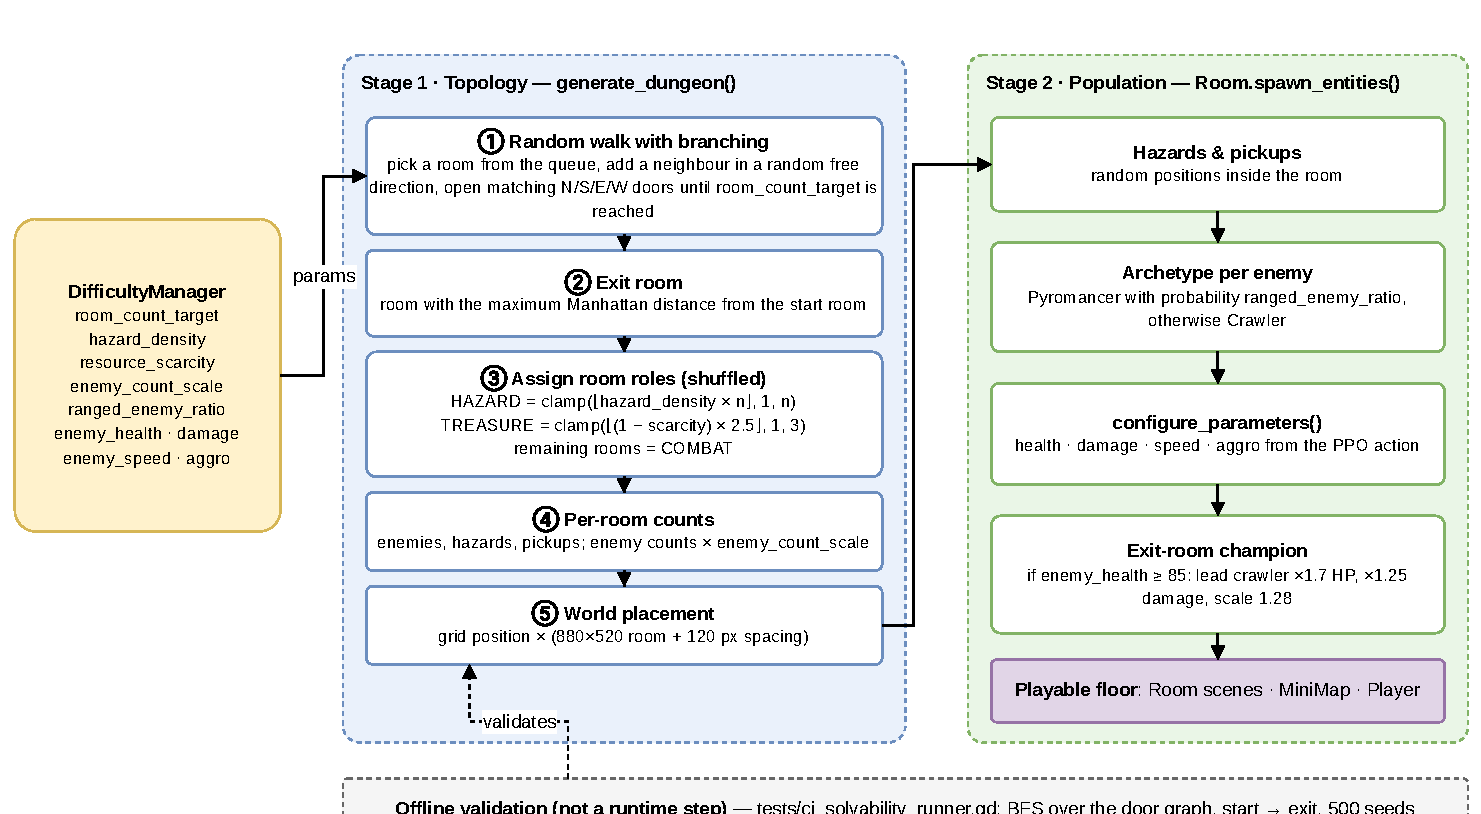
\includegraphics[width=0.95\textwidth]{ThesisFigs/fig_e_1_two_stage_procedural_pipeline}
\caption{Two-Stage Decoupled Procedural Generation Pipeline}
\label{fig:two_stage_detail}
\end{figure}

\section{Combat Feedback Event Flow}
Figure~\ref{fig:app_sprites} summarizes how gameplay events are turned into player-facing feedback in \texttt{Main.gd}, \texttt{Player.gd} and \texttt{Enemy.gd} (camera trauma, damage floaters, hit flashes, knockback and invulnerability frames), as implemented during Iteration 2.

\begin{figure}[!htbp]
\centering
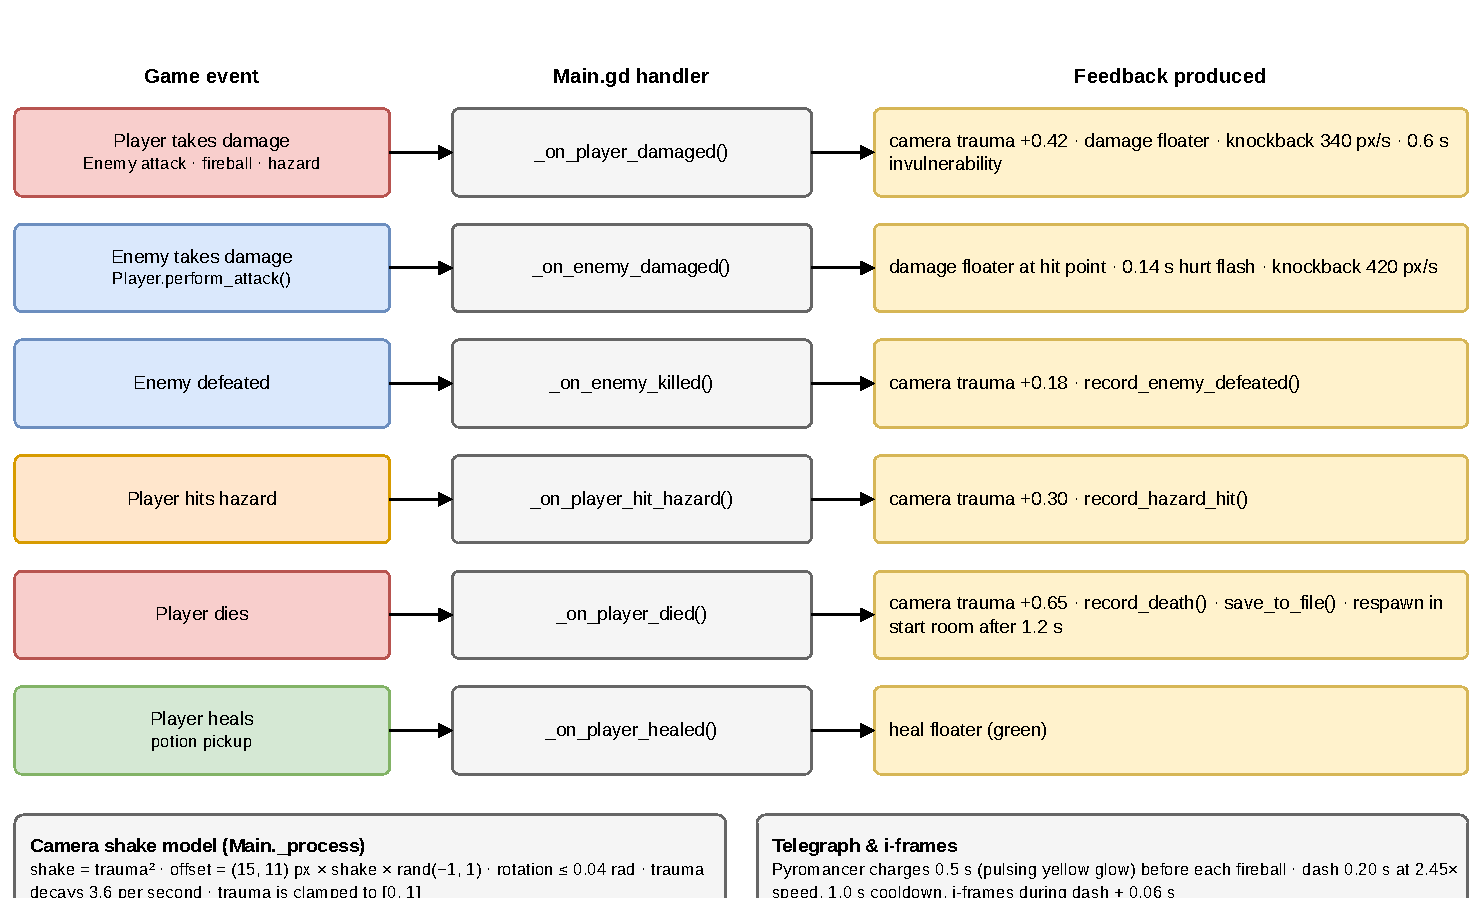
\includegraphics[width=0.95\textwidth]{ThesisFigs/fig_e_2_visual_asset_combat_feedback}
\caption{Combat Feedback Event Flow (event $\rightarrow$ handler $\rightarrow$ feedback)}
\label{fig:app_sprites}
\end{figure}

\chapter{Supervisory Meeting and Consultation Logs}
\label{app:meetings}

This appendix contains the official supervisory consultation records conducted with faculty supervisor \textbf{Ms. Mehreen Javaid}.

\section{Meeting Register}

{\small
\begin{longtable}{p{0.09\textwidth}p{0.17\textwidth}p{0.38\textwidth}p{0.28\textwidth}}
\toprule
\textbf{ID} & \textbf{Date} & \textbf{Agenda and Discussion Summary} & \textbf{Follow-up / Action Items} \\
M-01 & 2 Sep 2026 & Initial meeting: proposal of the FORGE project idea to the supervisor. & Refine the idea and prepare it for detailed discussion. \\
M-02 & 7 Sep 2026 & Discussion of the proposed idea: scope, approach and feasibility. & Consolidate scope and approach into the proposal. \\
M-03 & 9 Sep 2026 & Pre-defense meeting: review of the proposal and demo. & Finalize proposal, slides and demo. \\
M-04 & 23 Sep 2026 & Post-defense meeting: committee feedback and Mid-1 plan. & Address the committee directives (Table~\ref{tab:action_register}) in the Mid-1 deliverables. \\
M-05 & 5 Oct 2026 & Progress discussion for the Mid-1 evaluation (implementation and report). & Continue Mid-1 implementation and report writing. \\
M-06 & 7 Oct 2026 & Second progress discussion for the Mid-1 evaluation. & Continue Mid-1 implementation and report writing. \\
M-07 & 15 Oct 2026 & Pre-Mid-evaluation readiness check (demo, CI, report). & Final preparation for the Mid-1 evaluation. \\
\bottomrule
\end{longtable}
}


\bibliographystyle{IEEEtran}
\bibliography{references/references}
\end{document}
